\chapter{金属与能带绝缘体中的电子态}\label{chap:conventional-metal}

在几个冗长的、本质上是在回顾单粒子量子力学和群表示论的章节之后,我们开始分析一些实际的系统。
本章讨论那些电子重整化后形成可以辨认的电子型准粒子的系统,基本上就是传统意义上的“金属”、“绝缘体(为了和因为相互作用导致的或是杂质导致的绝缘体区分,通常称为\concept{能带绝缘体})”、“半导体”等。
本章的内容将足够解释常见的这些材料的行为——实际上,“有费米面的导电体”几乎可以成为金属的一个定义,而能带绝缘体因为只含有满带,其费米海的形状和第一布里渊区完全一样,而且费米能级附近根本没有电子模式,无法将费米能级附近的状态在动量空间中排列成一个几何体,总之,对能带绝缘体谈不上有费米面。

仔细想一下,金属中能够有可以辨认的电子型准粒子这件事是非常奇怪的:金属中的电子的库仑相互作用的量级通常和电子动能一样,似乎没有什么理由认为在如此强的相互作用下单电子模型能够适用。
然而实验的确告诉我们金属的行为在很多方面非常像费米气体,即实际上描述金属的低能有效理论基本上就是一个费米气体加上一定的相互作用修饰。

为什么对金属单电子图像有效仍然是并不完全清楚的问题。相互作用特别强烈以至于单电子图像不适用的系统是确确实实存在的(我们将在后文讨论它们),那么单电子图像适用就不是库仑相互作用电子系统必然会有的性质,具体怎样的晶体能够让单电子图像适用,怎样的晶体不行,仍然是有待研究的。

无论如何,实验事实告诉我们,对寻常的金属和能带绝缘体,我们可以以某种电子气——自由电子气,或者紧束缚模型等——为自由理论,以库伦相互作用为微扰,或者,可以使用这种凝聚态场论简化后得到的动理学,通常就是玻尔兹曼方程,这样可以避开完整的Keldysh场论而讨论一些非平衡问题。

本章将首先介绍能带电子的波包动力学和全量子力学处理,并首先使用玻尔兹曼方程、然后使用格林函数方法,计算电子间库伦排斥产生的影响,最后表明对相当一类系统,电子间库伦排斥只会让能带电子形成的费米气体变成费米液体。
费米液体在粒子数涨落不大的情况下,单粒子能谱和费米气体一样,热容、磁化率等和费米气体具有类似的形式,这反过来说明了单纯使用能带理论就能够足够精确地描述寻常的金属和能带绝缘体的原因,因此我们说,费米液体理论是\concept{能带论}的基础,这里的能带论指的是“系统的基本自由度可以近似看成能带电子”这一假设。

\section{外加电磁场下能带电子的准经典处理}

本节做如下近似:电子可以看成波包,要求它在动量空间比较局域,在实空间相对于晶格常数比较扩展,但是在宏观尺度上仍然足够局域。这通常要求原胞内的离子势没有剧烈变化,空间势的变化比较缓慢,外场没有破坏能带,外场变化足够慢,碰撞是瞬时发生的,散射较弱。 
它们的作用在后文的推导中可以看到。

\subsection{Bloch电子波包,波包动力学和半经典近似}\label{sec:bloch-wave-pocket}

考虑一个可以被看成晶格动量为$\vb*{k}_0$的Bloch电子波包。显然这个波包由同一个能带中的不同晶格动量成分组成(不同能带的电子具有非常不同的色散关系,它们各自运行的速度非常不同,用它们是无法组成一个比较稳定的波包的;以下略去能带标记$n$)。
注意波包的存在性本身就要求空间势的变化不能太剧烈,否则Bloch波函数在一个晶胞中将基本上定域在原子周围,无法形成比较“柔和”的波包。
波包中各个成分的晶格动量$\vb*{k}'$均很接近$\vb*{k}_0$,假定大体上
\begin{equation}
    - \frac{\Delta}{2} \leq k_i = k_{0i} - k'_i \leq \frac{\Delta}{2},
\end{equation}
从而可以做展开
\begin{equation}
    \epsilon_{\vb*{k}'} = \epsilon_{\vb*{k}_0} + \vb*{k} \cdot (\pdv*{\epsilon_{\vb*{k}}}{\vb*{k}})|_{\vb*{k}_0}.
\end{equation}
在没有外场时Bloch波函数是能量本征态,其时间演化是平凡的,它们叠加而成的波包的形式形如
\[
    \psi(\vb*{r}, t) = \sum_{\vb*{k}'} a_{\vb*{k}} \psi_{\vb*{k}'}(\vb*{r}, t) = \sum_{\vb*{k}'} a_{\vb*{k}} \ee^{\ii (\vb*{k}' \cdot \vb*{r} - \epsilon_{\vb*{k}'})} u_{\vb*{k}'}(\vb*{r}, t),
\]
其中$a_{\vb*{k}}$满足归一化条件。代入$\epsilon_{\vb*{k}'}$的展开式,能够得到以下近似表达式
\[
    \begin{aligned}
        \psi(\vb*{r}, t) &= \ee^{\ii (\vb*{k}_0 \cdot \vb*{r} - \epsilon_{\vb*{k}_0} t)} \sum_{\vb*{k}} a_{\vb*{k}} u_{\vb*{k}'}(\vb*{r}) \ee^{\ii \vb*{k} \cdot (\vb*{r} - (\pdv*{\epsilon_{\vb*{k}}}{\vb*{k}}) |_{\vb*{k}_0} t)} \\
        &= \ee^{\ii (\vb*{k}_0 \cdot \vb*{r} - \epsilon_{\vb*{k}_0} t)} u_{\vb*{k}_0}(\vb*{r}) \sum_{\vb*{k}} a_{\vb*{k}} \ee^{\ii \vb*{k} \cdot (\vb*{r} - (\pdv*{\epsilon_{\vb*{k}}}{\vb*{k}}) |_{\vb*{k}_0} t)}  ,
    \end{aligned}
\]
因此可以看出,波包前进的速度是$\pdv*{\epsilon_{\vb*{k}}}{\vb*{k}}$在$\vb*{k} = \vb*{k}_0$时的值。
这个对$\vb*{k}$的求和可以通过以下方式近似求出:我们认为% TODO

\begin{equation}
    \psi(\vb*{r}, t) = \ee^{\ii (\vb*{k}_0 \cdot \vb*{r} - \epsilon_{\vb*{k}_0} t)} u_{\vb*{k}_0}(\vb*{r}) % TODO
\end{equation}

$\Delta$是很小的,即$\Delta \ll 1 / a$,即
\begin{equation}
    \frac{1}{\Delta} \gg a,
\end{equation}
或者说,为了让波包描述有效,波包必须远大于原胞。这是合理的,因为如果使用波包的描述,我们是看不到晶格的,因此必须保证我们讨论的问题的尺度确实远大于晶格常数。

因此,结论是,一个“晶格动量大体上是$\vb*{k}_0$”的电子可以使用一个坐标$\vb*{r}$以及它的波函数的形状描述,其波函数是一个波包,在没有外场——从而系统的本征态就是Bloch电子——时,可以认为这个波包的运动速度由$\pdv*{\epsilon_{\vb*{k}}}{\vb*{k}}$给出。

现在考虑施加了外场的情况。我们之前假设过外场的空间变化不大,那么外场可以近似通过以下势场引入:
\[
    V = \vb*{r} \cdot \vb*{F}.
\]
与自由电子的情况不同,Bloch波矢$\vb*{k}$不能写成一个解析形式非常简单的算符的本征值,因此我们采取一个略微迂回的方法,考虑某个初基格矢$\vb*{a}$方向上的平移算符
\[
    T \ket{\vb*{r}} = \ket{\vb*{r} + \vb*{a}},
\]
Bloch波函数是它的本征态,有
\[
    T \psi_{n \vb*{k}} = \ee^{\ii \vb*{k} \cdot \vb*{a}} \psi_{n \vb*{k}},
\]
于是通过计算$\expval{T}$的演化方程就能够计算出外场存在时波包的$\vb*{k}$的演化方程。
我们有
\[
    \dv{\expval{T}}{t} = \expval{\ii \comm*{H}{T}} = \ii \expval*{\comm*{V}{T}}。
\]
通过对$\ket{\vb*{r}}$的作用可以验证
\[
    \comm*{x_i}{T} = a T,
\]
其中$x_i$指的是$\vb*{a}$方向上的$\vb*{r}$分量;其它$\vb*{r}$分量和$T$对易。
于是
\[
    \comm*{V}{T} = F_i a T.
\]
由于我们假定了波包在实空间非常舒展、在倒空间比较狭窄,可以认为
\[
    \expval*{T} = \ee^{\ii \vb*{k} \cdot \vb*{a}},
\]
于是$\expval*{T}$的时间演化方程最终转化为
\[
    \dv{t} \ee^{\ii \vb*{k} \cdot \vb*{a}} = \ii F_i a \ee^{\ii \vb*{k} \cdot \vb*{a}},
\]
就有
\[
    \ii \vb*{a} \cdot \dot{\vb*{k}} = \ii F_i a = \ii \vb*{a} \cdot \vb*{F}.
\]
将$\vb*{a}$取遍三个初基格矢就得到
\[
    \dot{\vb*{k}} = \vb*{F}.
\]
于是,我们就得到了
\begin{equation}
    \vb*{v} = \pdv{\epsilon_{\vb*{k}}}{\vb*{k}}, \quad \dv{\vb*{k}}{t} = \vb*{F},
\end{equation}
联立求解这组方程就获得了外场下的能带电子运动情况。
实际上,我们有
\[
    \dv{\vb*{v}}{t} = \dv{t} \pdv{\epsilon_{\vb*{k}}}{\vb*{k}} = \dv{\vb*{k}}{t} \cdot \pdv[2]{\epsilon_{\vb*{k}}}{\vb*{k}},
\]
即
\begin{equation}
    \dv{\vb*{v}}{t} = \frac{1}{m^*} \vb*{F}.
\end{equation}
这里的$m^*$正是\eqref{eq:effective-mass}中的有效质量。上式是各向异性版本的牛顿第二定律,不过要注意$m^*$\emph{不是}把$[\pdv*[2]{\epsilon_{\vb*{k}}}{k_i}{k_j}]_{ij}$中的每个元素取倒数,并且可能有对$\vb*{k}$的依赖;此外这里的$\vb*{k}$一直就是Bloch波矢而不是广延波矢。

在本节给出的准经典理论中不存在从一个能带到另一个能带的跃迁。运动学上看,这是因为含有多个能带分量的波包会很快分裂开来,而只含有一个能带分量的波包则是相对稳定的。
考虑电子的能谱,这是因为不同能带之间的能隙可以看成一个势垒,从而,一个波包到了能带边界会很快被弹回来。
在一些情况下能带之间的隧穿是很重要的,此时本节给出的理论必须加以修正。

本节使用同时确定$\vb*{p}$和$\vb*{r}$标记电子状态,这当然是有条件的,具体来说是电子的德布罗意波长要远小于外场发生变化的特征长度,由于会被激发的电子集中在费米面附近,有
\begin{equation}
    1 / k_\text{F} \ll L,
\end{equation}
其中$L$为外场发生变化的特征尺度;常常将外场在空间上做傅里叶变换,则上式等价于
\begin{equation}
    k_\text{F} \gg k,
\end{equation}
其中$k$是外场的动量尺度,大体上是$1/L$。

\subsection{外加电场下的电子振荡}

现在设一个恒定电场被加到晶体上,则会发生电子速度和晶格动量的振荡。
例如,考虑一个带底位于$\vb*{k}=0$处的能带,设$t=0$时电子在$\vb*{k}=0$处,由于是带底,有$\pdv*{\epsilon_{\vb*{k}}}{\vb*{k}} = 0$,即电子无速度,而$m^* > 0$,于是电子速度增加。
而到了布里渊区边界,由于晶格周期势场,能带变平,此时为带顶,由于$\pdv*{\epsilon_{\vb*{k}}}{\vb*{k}}$为零,电子速度为零,而由于是带顶,$m^* < 0$,于是电子被反向加速;注意此时$\vb*{k}$的变化方向还是沿着$\vb*{E}$的,$\vb*{k}$走出了第一布里渊区,或者等价地说,从第一布里渊区的另一侧进入了第一布里渊区。
这样,电子会从带底出发,首先被加速,到了一个$m^* = \infty$的地方时速度最大,然后减速,到了带顶速度正好降到零,然后$\vb*{k}$冲出第一布里渊区,而从第一布里渊区的另一侧回到第一布里渊区内,而$\vb*{v}$的方向则反了过来,最后回到带底。
在倒空间,电子从带底运动到带顶,然后从第一布里渊区的另一侧(也是带顶)回到带底;在实空间,出现能带倾斜,% TODO
这就是所谓的\concept{Bloch振荡}。

在实际实验中这个过程很难观察到,因为电子在运动中会不断受到介质中的其它准粒子和杂质的散射,这些本节没有考虑,而当电场强到电子运动得足够快,从而来不及被散射,让这种振荡得以发生时,往往或是材料被击穿,或是能带间隧穿会变得很明显,前一种情况下根本不能将介质看成晶体,后一种情况下波包动力学不可靠。
实际上,由于$\vb*{r}$和$\vb*{p}$的不对易性,在引入电场后严格来说就不能够让$\vb*{r}$和$\vb*{p}$同时出现。
我们此处所谓“能带在实空间中倾斜”的说法是建立在系统中没有任何东西有尖锐的空间变化,从而短距离看,似乎加入电场前后电子都处在Bloch态这一基础上的。
在这个假设被打破时——比如说,电势在空间中有急剧的变化,或者说有极强的电场时——波包动力学本来就不适用。

Bloch振荡的周期的量级和能带结构关系不大,而主要取决于晶格常数。电子在倒空间的运动速度为
\[
    \dv{k}{t} = e E,
\]
而第一布里渊区宽度大体上为$2 \pi / a$,因此
\begin{equation}
    \omega \sim e E a.
\end{equation}

\subsection{外加磁场下的电子振荡}

现在我们转而考虑有外加磁场时电子的响应,同样使用准经典的波包理论,并且忽略碰撞。
此时需要求解
\begin{equation}
    \vb*{v} = \pdv{\epsilon_{\vb*{k}}}{\vb*{k}}, \quad \dv{\vb*{k}}{t} = -e \vb*{v} \times \vb*{B}.
    \label{eq:calssical-magnetic-field}
\end{equation}
第二个方程意味着沿着磁场方向的$\vb*{k}$分量不发生改变,且由于洛伦兹力不做功,电子在$\vb*{k}$空间的运动轨迹是垂直磁场的平面与等能面的交线。
因此我们不做任何计算就确定了电子在倒空间中的行为。

例如,对自由电子可以解析求解以上方程,得到的是我们熟知的回转频率为
\begin{equation}
    \omega_0 = \frac{e B}{m}
\end{equation}
的螺旋运动。

\subsection{经典霍尔效应}\label{sec:classical-hall-effect}

首先考虑经典电动力学预言的霍尔效应。在有自由载流子的固体材料中电导率是一个张量。设我们在$y$方向施加一个电场$E_y$,并施加一个在$-z$方向的磁场$B$。
设载流子为电子,则稳态时电子应当朝左运动,且
\[
    \frac{e v B}{c} = e E_y,
\]
而电流方向朝右,大小为
\[
    j_x = - n_\text{e} e v = \frac{e c n_\text{e}}{B} E_y.
\]
我们将$\sigma_{xy}$这种横向的电导称为\concept{霍尔电导},记为
\begin{equation}
    \sigma_\text{H} = \frac{ec}{B} n_\text{e}.
\end{equation}

定义\concept{磁通量子}(它是超导中磁通量量子化的单位乘以2)
\begin{equation}
    \Phi_0 = \frac{h c}{e},
\end{equation}
一个电子绕着磁通量子整数倍的一个磁通量转一圈,不会产生可观测的效果(因为Berry相的变化是$2\pi$的整数倍)。
磁通量子是体系磁通量的一个自然的尺度。相应地,定义归一化磁通密度为
\begin{equation}
    n_{\Phi} = \frac{B}{\Phi_0},
\end{equation}
这给出了一个自然的电子数尺度,于是定义
\begin{equation}
    \nu = \frac{n_\text{e}}{n_\Phi} = \frac{n_\text{e} h c}{B e}.
\end{equation}
使用以上归一化之后的物理量,就可以写出霍尔电导为
\begin{equation}
    \sigma_\text{H} = \nu \frac{e^2}{h}.
\end{equation}
当然,到这里,$\nu$其实还是可以连续取值的。

\subsection{电子运动和碰撞的玻尔兹曼方程描述}

现在将电子-电子相互作用纳入考虑。

由于填满的能带中同时具有Bloch波矢为$\vb*{k}$和$-\vb*{k}$的电子,外加电场时它们运动方向相反,无导电性。

\subsubsection{Drude模型}

\subsection{热力学性质}

% TODO:Drude模型错误的热力学性质

金属中的准粒子主要就是电子和声子。按照\autoref{sec:lattice-special-heat},在极低温下声子能提供形如$T^3$的热容,而作为对比,极低温下电子热容正比于$T$(见\eqref{eq:free-electron-special-heat})。
因此在极低温下金属的比热主要由电子贡献,因为此时$T$相比$T^3$要明显。

\subsection{导电性和能带形式的分类}\label{sec:conductor-classification}

能带论能够解释为什么绝缘体不导电。自由电子气模型无法解释为什么绝缘体不导电——绝缘体中同样有大量的电子,似乎本应该导电。
% TODO:正向反向移动一样


现在可以根据导电性将较为寻常的、可以使用能带论解释的系统分类如下:
\begin{itemize}
    \item 电子的能带被完全填满的系统是绝缘体,称为\concept{能带绝缘体}。
    \item \concept{金属}就是有一些有电子的能带只是部分被填满的系统。
    \item \concept{半金属(semimetal)}是一些有电子的能带只有少量电子的系统,其导电性不好,但是仍然呈现一些金属的性质。
    \item \concept{半导体}是掺杂了的绝缘体,如果杂质能够形成能量大体上是在满带顶附近的局域空穴态,以及能量大体上是在空带底附近的局域电子态,那么热涨落就会让一些电子填充进空带中,而让满带中出现空穴,这就同时形成了两种载流子。
    不能依靠热涨落让电子从满带跳往空带,因为这要求费米温度量级的温度;我们需要掺杂才能够形成半导体。
\end{itemize}

在金属中,根据能带形状又可以分成这么几类:

使用$\xi_{\vb*{k}}$作为系统能量的定义,金属中的载流子——电子、空穴——在费米面附近是没有能隙的,因为$\xi_{\vb*{k}}$可以低到零,而能带绝缘体中的载流子是有能隙的。
本节讨论的都是近独立能带电子系统,因此载流子有能隙则系统有能隙,载流子无能隙则系统无能隙。
金属是无能隙的系统,因此其输运性质比有能隙的能带绝缘体要好。

\begin{figure}
    \centering
    \subfigure[金属的能带结构,费米能级在某一条能带内,有费米面,载流子在费米面上无能隙]{
        

\tikzset{every picture/.style={line width=0.75pt}} %set default line width to 0.75pt        

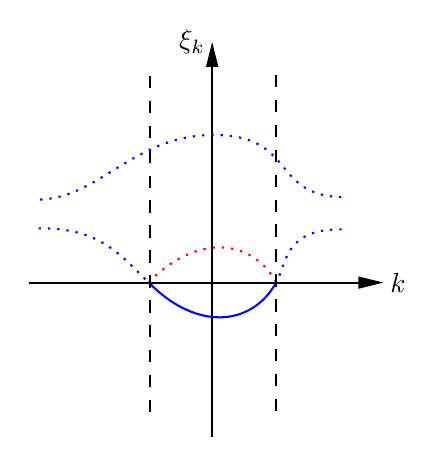
\begin{tikzpicture}[x=0.75pt,y=0.75pt,yscale=-1,xscale=1]
%uncomment if require: \path (0,300); %set diagram left start at 0, and has height of 300

%Straight Lines [id:da6538308978714695] 
\draw    (73.5,207.42) -- (242.29,207.42) ;
\draw [shift={(244.29,207.42)}, rotate = 180] [fill={rgb, 255:red, 0; green, 0; blue, 0 }  ][line width=0.08]  [draw opacity=0] (12,-3) -- (0,0) -- (12,3) -- cycle    ;
%Straight Lines [id:da5869056175210345] 
\draw    (161.89,281.81) -- (161.89,93.53) ;
\draw [shift={(161.89,91.53)}, rotate = 450] [fill={rgb, 255:red, 0; green, 0; blue, 0 }  ][line width=0.08]  [draw opacity=0] (12,-3) -- (0,0) -- (12,3) -- cycle    ;
%Curve Lines [id:da6300989437579545] 
\draw [color={rgb, 255:red, 0; green, 0; blue, 255 }  ,draw opacity=1 ] [dash pattern={on 0.84pt off 2.51pt}]  (79,167.42) .. controls (108.29,166.31) and (124.57,135.71) .. (163.79,136.31) .. controls (203,136.92) and (189.79,166.31) .. (226.29,166.31) ;
%Curve Lines [id:da8349659575379169] 
\draw [color={rgb, 255:red, 0; green, 0; blue, 255 }  ,draw opacity=1 ]   (131.29,207.31) .. controls (154.07,230.71) and (180.79,228.81) .. (192.79,207.31) ;
%Curve Lines [id:da5376843398312741] 
\draw [color={rgb, 255:red, 0; green, 0; blue, 255 }  ,draw opacity=1 ] [dash pattern={on 0.84pt off 2.51pt}]  (78.29,181.31) .. controls (107.79,180.81) and (117.79,194.31) .. (131.29,207.31) ;
%Curve Lines [id:da09130514197630113] 
\draw [color={rgb, 255:red, 0; green, 0; blue, 255 }  ,draw opacity=1 ] [dash pattern={on 0.84pt off 2.51pt}]  (224.29,181.81) .. controls (196.29,181.31) and (197.79,198.81) .. (192.79,207.31) ;
%Curve Lines [id:da8986151254017933] 
\draw [color={rgb, 255:red, 255; green, 0; blue, 0 }  ,draw opacity=1 ] [dash pattern={on 0.84pt off 2.51pt}]  (131.29,207.31) .. controls (154.07,183.92) and (180.79,185.81) .. (192.79,207.31) ;
%Straight Lines [id:da9787506067086109] 
\draw  [dash pattern={on 4.5pt off 4.5pt}]  (132,107.83) -- (132,270.94) ;
%Straight Lines [id:da2755726223329338] 
\draw  [dash pattern={on 4.5pt off 4.5pt}]  (192.5,107.39) -- (192.5,270.5) ;

% Text Node
\draw (159.89,91.53) node [anchor=east] [inner sep=0.75pt]    {$\xi _{\boldsymbol{k}}$};
% Text Node
\draw (246.29,207.42) node [anchor=west] [inner sep=0.75pt]    {$\boldsymbol{k}$};

\end{tikzpicture}

    }
    \subfigure[能带绝缘体的能带结构,费米能级不在任何一条能带内,无费米面,载流子有能隙]{
        

\tikzset{every picture/.style={line width=0.75pt}} %set default line width to 0.75pt        

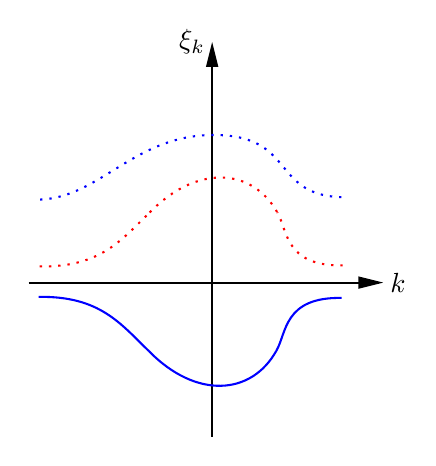
\begin{tikzpicture}[x=0.75pt,y=0.75pt,yscale=-1,xscale=1]
%uncomment if require: \path (0,300); %set diagram left start at 0, and has height of 300

%Straight Lines [id:da6739066413884267] 
\draw    (93.5,215.61) -- (262.29,215.61) ;
\draw [shift={(264.29,215.61)}, rotate = 180] [fill={rgb, 255:red, 0; green, 0; blue, 0 }  ][line width=0.08]  [draw opacity=0] (12,-3) -- (0,0) -- (12,3) -- cycle    ;
%Straight Lines [id:da018430257615266177] 
\draw    (181.89,290) -- (181.89,101.72) ;
\draw [shift={(181.89,99.72)}, rotate = 450] [fill={rgb, 255:red, 0; green, 0; blue, 0 }  ][line width=0.08]  [draw opacity=0] (12,-3) -- (0,0) -- (12,3) -- cycle    ;
%Curve Lines [id:da28208039701851084] 
\draw [color={rgb, 255:red, 0; green, 0; blue, 255 }  ,draw opacity=1 ] [dash pattern={on 0.84pt off 2.51pt}]  (99,175.61) .. controls (128.29,174.5) and (144.57,143.89) .. (183.79,144.5) .. controls (223,145.11) and (209.79,174.5) .. (246.29,174.5) ;
%Curve Lines [id:da011918462602831248] 
\draw [color={rgb, 255:red, 0; green, 0; blue, 255 }  ,draw opacity=1 ]   (151.29,248.5) .. controls (174.07,271.89) and (200.79,270) .. (212.79,248.5) ;
%Curve Lines [id:da7596938057105533] 
\draw [color={rgb, 255:red, 0; green, 0; blue, 255 }  ,draw opacity=1 ]   (98.29,222.5) .. controls (127.79,222) and (137.79,235.5) .. (151.29,248.5) ;
%Curve Lines [id:da41485246050791824] 
\draw [color={rgb, 255:red, 0; green, 0; blue, 255 }  ,draw opacity=1 ]   (244.29,223) .. controls (216.29,222.5) and (217.79,240) .. (212.79,248.5) ;
%Curve Lines [id:da8088044173967168] 
\draw [color={rgb, 255:red, 255; green, 0; blue, 0 }  ,draw opacity=1 ] [dash pattern={on 0.84pt off 2.51pt}]  (151.79,181.83) .. controls (174.57,158.44) and (201.29,160.33) .. (213.29,181.83) ;
%Curve Lines [id:da8927813193747982] 
\draw [color={rgb, 255:red, 255; green, 0; blue, 0 }  ,draw opacity=1 ] [dash pattern={on 0.84pt off 2.51pt}]  (98.79,207.83) .. controls (128.29,208.33) and (138.29,194.83) .. (151.79,181.83) ;
%Curve Lines [id:da9303631510934811] 
\draw [color={rgb, 255:red, 255; green, 0; blue, 0 }  ,draw opacity=1 ] [dash pattern={on 0.84pt off 2.51pt}]  (244.79,207.33) .. controls (216.79,207.83) and (218.29,190.33) .. (213.29,181.83) ;

% Text Node
\draw (179.89,99.72) node [anchor=east] [inner sep=0.75pt]    {$\xi _{\boldsymbol{k}}$};
% Text Node
\draw (266.29,215.61) node [anchor=west] [inner sep=0.75pt]    {$\boldsymbol{k}$};

\end{tikzpicture}

    }
    \caption{金属和能带绝缘体的能带结构,蓝色实线表示已经被占据的电子态,蓝色虚线表示没有被占据的电子态,红色虚线和蓝色实线沿着$x$轴轴对称,表示满的电子能带就是空的空穴能带}
\end{figure}

\section{外加电磁场下能带电子的量子理论}

\subsection{强磁场下电子的量子理论}

忽略晶格周期势场的半经典模型中磁场下的电子处于束缚态,因此可以预期,强磁场下将会出现明显偏离\eqref{eq:calssical-magnetic-field}的行为,半经典模型不再适用,因而值得单独拿出来处理。

\subsubsection{自由电子在磁场中的朗道能级}

我们采用\concept{对称规范},设磁场方向为$z$方向,且设
\begin{equation}
    A_x = - \frac{1}{2} B y, \quad A_y = \frac{1}{2} B x,
\end{equation}
这样通过
\[
    \vb*{B} = \curl{\vb*{A}}
\]
就得到一个$z$方向上大小为$B$的磁场。自由电子被放进磁场后,哈密顿量为
\begin{equation}
    {H} = \frac{\hbar^2}{2m} \left( - \ii \grad + \frac{e}{\hbar} \vb*{A} \right)^2.
    \label{eq:magnetic-hamiltonian}
\end{equation}
我们把$\hbar$放回了定义中,因为本节将需要频繁地用到这个能量尺度。
我们忽略了自旋与磁场的耦合,但是我们后面会发现这是无关紧要的。
\eqref{eq:magnetic-hamiltonian}中的导数被协变导数替代了,以满足$U(1)$对称性。
由于$z$方向没有$\vb*{A}$分量,实际上可以将\eqref{eq:magnetic-hamiltonian}当成\emph{二维}电子气的哈密顿量,电子在$xy$平面上处于束缚态,而在$z$方向和自由电子没有区别。
因此接下来我们讨论加入了磁场的二维自由电子气。

通过量纲分析可以发现\eqref{eq:magnetic-hamiltonian}中有一个特征长度
\begin{equation}
    l_0 = \sqrt{\frac{\hbar}{e B}},
\end{equation}
同时可以看出磁通量子确实是磁通量的一个尺度:
\[
    \Phi_0 = \frac{h}{e} \sim 2 B \pi l_0^2.
\]
这样,两个方向上的协变导数为
\begin{equation}
    D_x = \partial_x + \frac{\ii}{2l_0^2} y, \quad D_y = \partial_y - \frac{\ii}{2l_0^2}x.
\end{equation}
哈密顿量就转化为
\[
    {H} = - \frac{\hbar^2}{2m} (D_x^2 + D_y^2).
\]
容易验证$D_x$和$D_y$之间具有对易关系
现在定义
\begin{equation}
    D^\pm = D_x \pm \ii D_y,
\end{equation}
并定义复变量$z$为
\begin{equation}
    z = x + \ii y,
\end{equation}
则可以得到
\begin{equation}
    \comm*{D^-}{D^+} = - \frac{2}{l_0^2}.
\end{equation}
这意味着它们差一个常数就是一对升降算符。定义
\begin{equation}
    {a} = \ii \frac{l_0}{\sqrt{2}} D^-,
\end{equation}
就有
\begin{equation}
    {H} = \frac{\hbar^2}{m l_0^2} \left({a}^\dagger {a} + \frac{1}{2} \right) = \hbar \omega_0 \left({a}^\dagger {a} + \frac{1}{2} \right).
    \label{eq:landau-energy-level}
\end{equation}
因此系统具有分立的能级,称为\concept{朗道能级},其中
\begin{equation}
    \omega_0 = \frac{eB}{m}
\end{equation}
正是经典图景中电子在磁场下做匀速圆周运动的圆频率。
在磁场很弱的时候,这个能谱接近连续,此时可以使用\eqref{eq:magnetic-hamiltonian}。
而在磁场很强时就有明显的分立的能级,且能级间距远大于$\hbar B$,从而自旋-磁场耦合导致的能级分裂\emph{可以忽略}。
把$z$方向的运动加上,就是
\begin{equation}
    {H} = \frac{\hbar^2}{m l_0^2} \left({a}^\dagger {a} + \frac{1}{2} \right) + \frac{p_z^2}{2m} = \hbar \omega_0 \left({a}^\dagger {a} + \frac{1}{2} \right) + \frac{\hbar^2 k_z^2}{2m}.
    \label{eq:landau-energy-3d}
\end{equation}

实际上,朗道能级对应的波函数可以写成一个全纯函数乘以一个高斯因子。设$\Psi$是基态波函数,我们做拟设
\begin{equation}
    \Psi(x, y) = f(z, z^*) \ee^{- z z^* / 4l_0^2},
    \label{eq:landau-wave-packet}
\end{equation}
由于
\[
    D^- \Psi = 0,
\]
展开计算可以发现
\[
    \pdv{f}{z^*} = 0,
\]
这表明$f$一定是全纯函数,即得所求证。

\subsubsection{二维电子气在强磁场下的行为}\label{sec:2d-electron-magnetic-field}

我们现在考虑$z$方向高度受限的一个系统,即考虑一个真正的自由二维电子气在强磁场下的行为。
自由二维电子气的$\vb*{k}$分布在平面上,其“费米面”实际上是费米圆。
现在讨论二维电子气的朗道能级的简并度。有一点是可以确定的:朗道能级的简并度非常高,因为原本准连续的$k_x, k_y$被“压缩”到了分立的朗道能级上。二维平面上自由电子计入自旋的态密度为
\begin{equation}
    \dv{n}{\epsilon} = 2 \times \int \dd{l} \frac{1}{\abs{\pdv*{\epsilon_{\vb*{k}}}{\vb*{k}}}} = \frac{m S}{\pi \hbar^2},
\end{equation}
单个朗道能级的简并度是
\begin{equation}
    D = \frac{m S}{\pi \hbar^2} \times \hbar \omega_0 = \frac{S e}{\pi \hbar} B.
\end{equation}
直观地看,原本连续的二维自由电子能带被分割成了若干长度为$\hbar \omega_0$的小段,每个小段被“压缩”到一个朗道能级上;每个小段上的能量平均值和对应的朗道能级的能量刚好一样。

一个能够赋予明确的半经典意义的数量级估计如下。
\eqref{eq:landau-wave-packet}给出了一个特征长度为$l_0$的波包。当然,将一个波包做平移之后还是可以得到一个波包。两个波包如果不重叠,就是彼此正交的系统的本征态。
设体系总面积为$S$,我们可以认为体系被分割成了一系列大小为$\pi l_0^2$的圆,于是简并度为
\[
    \frac{S}{\pi l_0^2} \sim S \frac{eB}{h c} = \frac{\Phi}{\Phi_0}.
\]
其中定义
\begin{equation}
    \Phi_0 = \frac{h c}{e}
\end{equation}
为\concept{磁通量子}。

实际上,根据半经典理论,有
\[
    \frac{\hbar^2 k^2}{2m} = \hbar \omega_0 n,
\]
因此第$n$能级在动量空间中画出的圆的面积是
\begin{equation}
    S_k^n = \pi k_n^2 = \frac{2 \pi e}{\hbar} B n,
\end{equation}
因此相邻两个能级的倒空间中的圆的面积差(是一个环)是
\begin{equation}
    \Delta S_k = \frac{2 \pi e}{\hbar} B.
\end{equation}
既然运动方程为
\[
    \hbar \dd{\vb*{k}} = - e \dd{\vb*{r}} \times \vb*{B},
\]
有
\begin{equation}
    \Delta S_r = \frac{2\pi \hbar}{eB}.
\end{equation}

注意到由于$\Psi(\vb*{r})$可以被恰当地归一化,它在电子气占据的范围内不应该有任何奇点,于是可以做泰勒展开
\[
    f(z) = c_0 + c_1 z + c_2 z^2 + \cdots,
\]
实际上可以证明,$\{z^m \ee^{- \abs{z}^2 / 4 l_0^2}\}$构成一组完备正交基。
现在寻找波函数幅值最大的位置,即计算
\[
    \pdv{\abs{\Psi_n(\vb*{r})}^2}{r} = 0
\]
的解,其解为
\[
    r_n = \sqrt{2n} l_0.
\]
换而言之我们得到了一组年轮一样的基矢量。设基态简并度为$n$则
\[
    S = \sqrt{2n} l_0,
\]
从而
\[
    n = S \cdot \frac{eB}{\hbar c} = \frac{\Phi}{\Phi_0}.
\]

在磁场很大时,我们有若干高度简并,同时彼此之间有明显间距的离散能级。$B$增大会让能级间距线性增大,同时让单能级简并度线性增大,于是总的模式数目保持不变。

二维电子气的费米能级实际上会导致一个很有趣的现象:缓慢增大或是减小磁场然后待系统达到平衡,系统能量会发生变化。
如果在某个磁场值$B_0$下正好前$\lambda$个朗道能级被填满,通过数模式数目会发现这些电子模式在无磁场的情况下占据的最高能级的能量正好就是$(\lambda + 1) \hbar \omega_0$,计算系统总能量,发现和磁场为$B_0$时的系统总能量正好一样。
现在略微降低磁场,朗道能级间距缩短,从而一些电子在平衡时需要占据$\lambda+1$能级,因此加入磁场后系统能量升高了。
容易看出当第$\lambda+1$能级刚好占据了一半的时候系统能量比加入磁场前增大得最多。
进一步增大磁场,会发现一部分在自由情况下能量高于$\lambda+1$能级的能量的电子也需要填充在$\lambda+1$能级上,不过这部分电子的数目少于自由情况下能量低于$\lambda+1$的电子的数目,因此此时加入磁场后系统能量仍然上升,但是上升的量和第$\lambda+1$能级刚好占据了一半的情况比起来不那么大了。

总之,如此周而往复,只要加入磁场,系统的平衡态能量就不会低于自由时的能量,且每当有某个磁场使得对应的某个朗道能级满足($\epsilon_\text{F}$是加入磁场前的费米能级)
\begin{equation}
    \left( n + \frac{1}{2} \right) \hbar \omega_0 = \epsilon_\text{F}
\end{equation}
时系统能量相对于加入磁场前的增量达到峰值,而
\begin{equation}
    n \hbar \omega_0 = \epsilon_\text{F}
\end{equation}
或者说$n D$是总电子数$N_\text{e}$时系统能量和加入磁场前相比没有什么变化。代入$\omega_0$会发现
\[
    n \frac{S e}{\pi \hbar} B = N_\text{e},
\]
因此实际上以上系统能量的变化相对于$1/B$是周期性的,周期为
\begin{equation}
    \Delta\left(\frac{1}{B}\right) = \frac{Se}{\pi \hbar N_\text{e}} = \frac{2\pi e}{\hbar S_\text{F}},
    \label{eq:de-hass-van-alphen-period}
\end{equation}
其中
\begin{equation}
    S_\text{F} = 2 \pi^2 \frac{N_\text{e}}{S}
\end{equation}
是二维电子气费米圆的面积。

很多东西都依赖于系统总能量,如磁矩定义为$- \pdv*{E}{B}$,照以上推导,它也应该关于$1/B$以周期\eqref{eq:de-hass-van-alphen-period}变化。这称为\concept{de Hass-van Alphen效应}。比热等物理量也有这个关系。

% TODO:二维电子气的半经典kx和ky

\subsubsection{三维电子气在强磁场下的行为}

一个$z$方向可以充分延展的系统,即一个三维电子气,在强磁场下的行为还要复杂一些。
在与磁场垂直的$k_z=\const$的平面内轨道按照\eqref{eq:landau-energy-3d}是分立的,而$z$方向上的$k_z$是连续的。
$xy$平面上没有良定义的Bloch波矢,但是还是可以根据二维情况中的说法计算出准经典的$k_x$和$k_y$。
于是我们可以将三维电子气中的各个模式形象地在倒空间中展示为一系列同心圆柱面,一个模式的$\vb*{k}$总是固定在某个同心圆柱面上,其$k_z$不变,而$k_x$和$k_y$随着时间变化连续旋转,没有确定的值。
好量子数有两个,一个是区分不同同心圆柱面的$n$,一个是$z$方向的$k_z$。

一维电子气的轨道态密度是
\begin{equation}
    g(\epsilon_{k_z}) = \frac{L \sqrt{2m}}{2 \pi \hbar} \epsilon_{k_z}^{-1/2},
\end{equation}
由于强磁场下可以忽略自旋导致的能级分裂而有两种自旋这件事已经充分体现在了$D$当中,所有子带的态密度(同时包括自旋和轨道)的总和就是
\begin{equation}
    g(\epsilon) = D \frac{L \sqrt{2m}}{2 \pi \hbar} \sum_n \left(\epsilon - \left( n + \frac{1}{2} \right) \hbar \omega_0 \right)^{-1/2}.
\end{equation}

在三维电子气中我们也可以观察到de Hass-van Alphen效应,虽然不是严格成立的。
% TODO:绘图
当费米球和某个圆柱面相切时系统能量增量最大。

\section{高密度电子气的静电屏蔽和RPA近似}

\subsection{托马斯-费米静态屏蔽势}\label{sec:ext-e}

本节讨论的系统满足所谓\concept{托马斯-费米近似}:在其中,电子充分稠密,从而相互作用能非常强,电子凭借其自身的动能无法远距离传播,从而系统状态可以使用电子数密度$n(\vb*{r})$标记%
\footnote{
    很明显由于$\vb*{r}$和$\vb*{p}$不对易,如果我们想要有有意义的$\vb*{k}$表象,系统中所有依赖于$\vb*{r}$的量在空间上都必须变化得足够平缓。
    这和前面的波包动力学中外加电场时的条件是一个道理。
    \label{note:smooth-electron-distribution}
}%
,且相互作用能可以完全认为是来自密度-密度相互作用即Hartree项,而忽略交换作用等除此以外的效应。
由于可以忽略交换作用,可以完全照搬经典静电学,即认为一个电子的全部能量是其动能加上电势能,而不考虑任何交换能或者关联能。
想象我们在一个满足托马斯-费米近似的近独立电子气当中放入一个电荷。显然,异号电荷会移动到前者附近而产生一个屏蔽效应。
在电子气规模很大时(我们所研究的固体总是在热力学极限之下,因此这是成立的),屏蔽效应很强,这让外加电荷对电子气的扰动实际上局限在外加电荷的一个小邻域内。
于是求解外加电荷的影响就是求解以下自洽问题:
\begin{enumerate}
    \item 外加电荷导致外加电势能
    \begin{equation}
        \phi_\text{ext} = \frac{Q}{r},
    \end{equation}
    \item 外加电势与屏蔽电荷形成的电势$\var{\phi}$叠加,导致总的电势变化为
    \begin{equation}
        \phi_\text{eff} = \phi_\text{ext} + \var{\phi},
    \end{equation}
    \item 总电势变化$\phi_\text{eff}$导致了电荷密度变化$\var{n}$,电荷密度变化给出屏蔽电势$\var{\phi}$。
\end{enumerate}
自洽求解以上问题就可以确定所有物理量。

以上自洽求解步骤还需要一个方程:$V_\text{eff}$是怎么影响电荷密度的。
$V_\text{eff}$改变粒子排布的方式是这样的:单电子的能量$\epsilon_{\vb*{k}}$会由于$V_\text{eff}$的引入发生一个小的变化,且这个小的变化在不同位置通常是不一样的。
由于托马斯-费米近似成立,我们认为每个$\vb*{r}$位置附近的诸电子都可以认为是组成了一个正则系综%
\footnote{这么做总是可以的,因为我们讨论近平衡态理论,确实允许电荷密度在空间上出现分布,虽然完全的平衡态电子气应该是均匀的。}%
,且$\vb*{k}$和$\vb*{r}$可以同时确定,于是
\[
    n(\vb*{r}) = \sum_{\vb*{k}, \sigma} \frac{1}{1 + \ee^{\beta (\epsilon_{\vb*{k}}(\vb*{r}) - \mu)}} = 2 \sum_{\vb*{k}} \frac{1}{1 + \ee^{\beta (\epsilon_{\vb*{k}}(\vb*{r}) - \mu)}}, \quad \epsilon_{\vb*{k}}(\vb*{r}) = \epsilon_{\vb*{k}}^0 + V_\text{eff}(\vb*{r}),
\]
由于体系足够大,屏蔽作用让外加电荷的作用几乎是局域的,则$\var{n}(\vb*{r})$可以写成$V_\text{eff}(\vb*{r})$的函数而不涉及长程相互作用。
而由于外加电荷很小,可以采取线性近似,于是(第二个等号是因为费米-狄拉克分布的形式)
\[
    \var{n} = \dv{n}{V_\text{eff}} V_\text{eff} = \sum_{\vb*{k}} \pdv{n}{\epsilon_{\vb*{k}}} V_\text{eff} = - \pdv{n}{\mu} V_\text{eff},
\]
关于能量的态密度(即单位$\dd{\epsilon}$、单位体积中有多少可能的态)为
\begin{equation}
    N(\mu' - \mu) = \pdv{n\big|_{\mu \to \mu'}}{\mu'},
\end{equation}
其中能量从费米面量起,且我们将$n$的表达式中的$\mu$换成了变量$\mu'$,而使用$\mu$表示实际系统的化学势。使用该记号,则
\begin{equation}
    \var{n}(\vb*{r}) = - N(0) V_\text{eff}(\vb*{r}).
    \label{eq:from-veff-to-varn}
\end{equation}
这就是从$V_\text{eff}$计算$\var{n}$的方法。通过$\var{n}$计算$\var{\phi}$的方程为泊松方程
\[
    - \laplacian \phi_\text{eff} = 4 \pi \left( Q \delta(\vb*{r}) - e \var{n}(\vb*{r}) \right),
\]
其中我们不失一般性地将外加电荷放在原点上。使用傅里叶变换并且使用$\var{n}$和$V_\text{eff}$之间的线性关系\eqref{eq:from-veff-to-varn},可以得到
\[
    k^2 V_\text{eff}(\vb*{k}) = - 4\pi e Q - 4 \pi e^2 N(0) V_\text{eff}(\vb*{k}),
\]
解出$V_\text{eff}(\vb*{k})$为
\[
    V_\text{eff}(\vb*{k}) = - \frac{4 \pi e Q}{k^2 + \kappa
    _\text{TF}^2},
\]
做傅里叶逆变换得到
\begin{equation}
    V_\text{eff}(\vb*{r}) = - \frac{eQ}{r} \ee^{- \kappa_\text{TF} r},
    \label{eq:thomas-fermi-potential}
\end{equation}
其中
\begin{equation}
    \kappa_\text{TF}^2 = 4 \pi e^2 N(0).
\end{equation}
这个结果就是\concept{托马斯-费米屏蔽}。

\subsection{RPA近似下的动态屏蔽响应}

\begin{back}{线性响应理论中的格林函数}{linear-response-green-function}
    凝聚态理论中计算最多的是线性响应理论中的格林函数。所谓线性响应理论是说,设时间平移不变的系统受到外加哈密顿量
    \begin{equation}
        H_\text{ext} = h(t) A
    \end{equation}
    扰动,只考虑系统的密度矩阵正比于$h(t)$的变化,则算符$B$的期望值由
    \begin{equation}
        y(t) = \int \dd{t'} G^\text{ret}_{AB}(t, t') h(t'), \quad y(t) = \expval{B}(t) - \expval{B}_0
    \end{equation}
    给出,其中
    \begin{equation}
        G^\text{ret}_{AB}(t-t') = - \ii \theta(t-t') \expval{[B(t), A(t')]}_0
    \end{equation}
    是有限温度推迟格林函数,其中$\expval{\cdot}$表示考虑了$H_\text{ext}$的期望而$\expval{\cdot}_0$表示没有考虑$H_\text{ext}$的期望。
    不过因为我们在做实际计算时通常都使用没有考虑$H_\text{ext}$的哈密顿量,以下会略去下标$0$。

    推迟格林函数不易直接计算,因为它不是编时格林函数,因此不能直接使用Wick定理。通常我们会使用松原格林函数辅助计算。
    松原格林函数为
    \begin{equation}
        G_{AB}(\tau) = - \timeorder \expval*{A(\tau) B(0)}, \quad G_{AB}(\ii \omega_n) = \int_0^\beta \dd{\tau} \ee^{\ii \omega_n \tau} G_{AB}(\tau),
    \end{equation}
    从频域切换回虚时间的方法是
    \begin{equation}
        G_{AB}(\tau) = \frac{1}{\beta} \sum_{\omega_n} G_{AB}(\ii \omega_n) \ee^{- \ii \omega_n \tau}.
    \end{equation}
    对自由理论,有
    \begin{equation}
        G^{0}(\ii \omega_n) = - \int_0^\beta \dd{\tau} \ee^{\ii \omega_n \tau} \timeorder \expval*{c(\tau) c^\dagger(0)} = \frac{1}{\ii \omega_n - \epsilon}.
    \end{equation}
    做费曼图计算时应当注意传播子是$-G^{0}_{AB}(\ii \omega_n)$。
    从松原格林函数延拓到实时间推迟格林函数的方法是将$\ii \omega_n$替换成$\omega + \ii 0^+$。

    形式上,我们可以对$\tau$做Wick转动$\tau = \ii t$,这样的理论和高能物理中常用的零温场论形式上完全一样,后者的格林函数定义为
    \begin{equation}
        \ii G_{AB}(t) = \timeorder \expval*{A(t) B(0)}, \quad G_{AB}(\omega) = \int \dd{t} \ee^{\ii \omega t} G_{AB}(t),
    \end{equation}
    对自由理论,有
    \begin{equation}
        G^0(\omega) = \frac{1}{\omega - \epsilon}.
    \end{equation}
    % TODO:含有二阶求导的情况

    近独立电子气的格林函数和它的谱函数是可以比较容易地算出的。松原格林函数为
    \begin{equation}
        G(\vb*{k}, \ii \omega_n) = - \int_0^\beta \dd{\tau} \ee^{\ii \omega_n \tau} \timeorder \expval*{c_{\vb*{k}}(\tau) c_{\vb*{k}}^\dagger(0)} = \frac{1}{\ii \omega_n - \epsilon_{\vb*{k}}},
    \end{equation}
    推迟格林函数为
    \begin{equation}
        G^\text{ret}(\vb*{k}, \omega) = \frac{1}{\omega - \epsilon_{\vb*{k}} + \ii 0^+},
    \end{equation}
    谱函数为
    \begin{equation}
        A(\vb*{k}, \omega) = \delta(\omega - \epsilon_{\vb*{k}}).
    \end{equation}
    这些都和单电子计算出来的结果完全一样。
\end{back}

托马斯-费米屏蔽是静态的。现在考虑一般的近独立电子气的线性响应。
外加电势导致如下的相互作用哈密顿量:
\[
    {H}_\text{ext} = \int \dd[3]{\vb*{r}} {n}(\vb*{r}, t) V_\text{ext} (\vb*{r}, t),
\]
则它对电子数密度的影响可以使用(各向同性不含时体系的)推迟格林函数
\[
    G^\text{ret}_{nn}(\vb*{r}-\vb*{r}', t-t') = - \ii \theta(t-t') \expval*{\comm{\var{{n}}(\vb*{r}, t)}{\var{{n}}(\vb*{r}', t')}}
\]
描述,而响应就是%
\footnote{我们没有将$V_\text{ext}$写进${H}$中而是把它看成了外界扰动,这样电子气本身的哈密顿量仍然是空间平移不变的。}%
\begin{equation}
    \expval*{\var{{n}}(\vb*{r}, t)} = \int \dd{t'} G^\text{ret}_{nn}(\vb*{r}-\vb*{r}', t-t') V_\text{ext}(\vb*{r}', t'),
\end{equation}
在频域中就是
\begin{equation}
    \expval*{\var{{n}}(\vb*{k}, \omega)} = G^\text{ret}_{nn}(\vb*{k}, \omega) V_\text{ext}(\vb*{k}, \omega).
    \label{eq:green-function-electro-shielding}
\end{equation}
当然,在系统的构成已知的情况下,可以直接用费曼图计算出格林函数$G^\text{ret}_{nn}$,但是本节不这么处理问题。
但如果真的这么做很快就会遇到数学上的困难:费曼图求和需要经过一些特殊的重求和步骤才能够给出有意义的结果。
因此本节只是做一个近似,将最为奇异的那部分费曼图做一个求和,然后发现它确实能够给出有意义的结果。

为简化问题我们做\concept{RPA(Random Phase Approximation)近似}%
\footnote{这个名称最早来自核物理,在那里它是通过对某个随机相位的求和得到的。}%
,这个近似要求以下两点:
\begin{itemize}
    \item $\var{{n}}$和$V_\text{eff}$之间的响应函数近似是自由电子的$\var{{n}}$-$\var{{n}}$格林函数,即我们认为$V_\text{eff}$中来自电子屏蔽的部分在其它电子上的作用和一个外加势场完全没有区别;
    \item 只考虑经典静电能,即将电子数密度期望当成经典电子数密度,忽略所有交换能或关联能。
\end{itemize}
RPA近似看起来似乎没有什么明确的意义,但它实际上把最为奇异剧烈效应考虑在内,并且给出了定性上正确的屏蔽库伦势(从一个长程的相互作用变成了一个短程的相互作用)。如果RPA近似不准,只需要多算几个微扰就可以。
这样,自洽方程可以通过下面的方法给出。
\begin{enumerate}
    \item 外加电荷引入外加电势能,
    \item 外加电势能加上屏蔽电荷产生的电势能等于总的电势能变化$V_\text{ext}$,
    \item 总的电势能变化可以反推出屏蔽电荷。
\end{enumerate}

粒子数的平均值近似为一个经典的数密度,从而$\var{V}$可以使用泊松方程写成
\[
    - \laplacian \var{V}(\vb*{r}, t) = - 4\pi e^2 \expval*{\var{{n}}(\vb*{r}, t)},
\]
也即
\begin{equation}
    k^2 \var{V}(\vb*{k}, \omega) = 4\pi e^2 \expval*{\var{{n}}(\vb*{k}, \omega)}.
\end{equation}
于是第二步完成了。

第三步通过RPA近似的基本假设得到。这里我们用$G^\text{0, ret}_{nn} (\vb*{k}, \omega)$作为$G^\text{0, ret}_{\var{n}\var{n}} (\vb*{k}, \omega)$的简写:
\begin{equation}
    \expval*{\var{{n}}(\vb*{k}, \omega)} = G^\text{0, ret}_{nn} (\vb*{k}, \omega) V_\text{eff} (\vb*{k}, \omega).
    \label{eq:rpa-approximation}
\end{equation}
这样就得到自洽方程
\[
    V_\text{ext}(\vb*{k}, \omega) + \frac{4\pi e^2}{k^2} \expval*{\var{{n}}(\vb*{k}, \omega)} = (G^\text{0, ret}_{nn} (\vb*{k}, \omega))^{-1} \expval*{\var{{n}}(\vb*{k}, \omega)},
\]
从而
\begin{equation}
    G^\text{ret}_{nn}(\vb*{k}, \omega) = \frac{G^\text{0, ret}_{nn}(\vb*{k}, \omega)}{1 - \frac{4\pi e^2}{k^2} G^\text{0, ret}_{nn}(\vb*{k}, \omega)} = \frac{G^\text{0, ret}_{nn}(\vb*{k}, \omega)}{\epsilon(\vb*{k}, \omega)},
    \label{eq:ext-electron-ret-nn}
\end{equation}
其中$\epsilon(\vb*{k}, \omega)$是介电常数。
这样,计算出自由电子的密度-密度格林函数之后问题就完全解决了。

由于自旋守恒性,只有$\sigma = \sigma'$的项才非零,我们得到
\[
    G_{nn}^\text{0}(\vb*{r}-\vb*{r}', \tau-\tau') = \sum_\sigma G_\sigma(\vb*{r}' - \vb*{r}, \tau' - \tau) G_\sigma(\vb*{r} - \vb*{r}', \tau - \tau').
\]
上式具有卷积的形式,切换到频谱,就是
\[
    G_{nn}^\text{0}(\vb*{q}, \ii \omega_n) = \sum_{\sigma} \sum_{\vb*{k}} \frac{1}{\beta} \sum_{\nu_n} G_\sigma(\vb*{q}, \ii \nu_n) G_\sigma(\vb*{k} + \vb*{q}, \ii (\omega_n + \nu_n)),
\]
其中
\[
    \nu_n = \frac{\pi(2n+1)}{\beta}, \quad \omega_n = \frac{2\pi n}{\beta},
\]
前者是费米子的松原频率,后者则是玻色子的,因为电子配对形成玻色子。自由费米子的谱函数为
\[
    A(\vb*{k}, \omega) = \delta(\omega - \xi_{\vb*{k}}), \quad \xi_{\vb*{k}} = \frac{\vb*{k}^2}{2m} - \mu,
\]
格林函数为
\[
    G_\sigma(\vb*{r}, \ii \omega_n) = \frac{1}{\ii \omega_n - \xi_{\vb*{k}}}.
\]
于是,有
\[
    G_{nn}^\text{0}(\vb*{q}, \ii \omega_n) = 2 \sum_{\vb*{k}} \frac{1}{\beta} \sum_{\nu_n} \frac{1}{\ii \nu_n - \xi_{\vb*{k}}} \frac{1}{\ii \omega_n + \ii \nu_n - \xi_{\vb*{k}+\vb*{q}}}.
\]
要计算上式,常用的一个技巧是将求和转化为围道积分。注意到$\{\ii \nu_n\}$正是$f(z)$的全部极点,而且这些极点都是一阶极点。
容易看出这些极点的留数都是$-1/\beta$,于是对一个在虚轴上解析的函数$F(z)$,有
\[
    \frac{1}{\beta} \sum_{\nu_n} F(\ii \nu_n) = - \oint \frac{\dd{z}}{2\pi \ii} f(z) F(z),
\]
于是设围绕虚轴的环路为$C$,它实际上就是从$-\ii \infty + 0^+$到$\ii \infty + 0^+$,再从$\ii \infty - 0^+$到$-\ii \infty - 0^+$,
有
\[
    \begin{aligned}
        G_{nn}^\text{0}(\vb*{q}, \ii \omega_n) &= - 2 \sum_{\vb*{k}} \oint_C \frac{\dd{z}}{2\pi \ii} f(z) \frac{1}{z - \xi_{\vb*{k}}} \frac{1}{z +  \ii \omega_n - \xi_{\vb*{k}+\vb*{q}}} \\
        &= 2 \sum_{\vb*{k}} \left( \frac{f(\xi_{\vb*{k}})}{\xi_{\vb*{k}} + \ii \omega_n - \xi_{\vb*{k} + \vb*{q}}} + \frac{f(\xi_{\vb*{k} + \vb*{q}} - \ii \omega_n)}{\xi_{\vb*{k} + \vb*{q}} - \ii \omega_n - \xi_{\vb*{k}}} \right).
    \end{aligned}
\]
负号消失了是因为绕极点$z=\xi_{\vb*{k}}$和$z = \xi_{\vb*{k} + \vb*{q}} - \ii \omega_n$是顺时针而不是留数定理通常是的逆时针(见\autoref{fig:rpa-pole})。
由$\{\omega_n\}$的定义,$f(\xi_{\vb*{k} + \vb*{q}} - \ii \omega_n)$就是$f(\xi_{\vb*{k} + \vb*{q}})$,于是得到松原格林函数
\begin{equation}
    G_{nn}^\text{0}(\vb*{q}, \ii \omega_n) = 2 \sum_{\vb*{k}} \frac{f(\xi_{\vb*{k}}) - f(\xi_{\vb*{k} + \vb*{q}})}{\ii \omega_n + \xi_{\vb*{k}} - \xi_{\vb*{k} + \vb*{q}}}.
\end{equation}
做解析延拓就得到推迟格林函数
\begin{equation}
    G_{nn}^\text{ret, 0}(\vb*{q}, \ii \omega_n) = 2 \sum_{\vb*{k}} \frac{f(\xi_{\vb*{k}}) - f(\xi_{\vb*{k} + \vb*{q}})}{\omega + \xi_{\vb*{k}} - \xi_{\vb*{k} + \vb*{q}} + \ii 0^+}.
    \label{eq:ext-electron-retarded-green-function}
\end{equation}
介电常数为
\begin{equation}
    \epsilon(\vb*{k}, \omega) = \frac{V_\text{ext}}{V_\text{eff}} = 1 - \frac{4 \pi e^2}{k^2} G^\text{ret, 0}_{nn}(\vb*{k}, \omega)
\end{equation}

\begin{figure}
    \centering
    \tikzset{every picture/.style={line width=0.75pt}} %set default line width to 0.75pt        

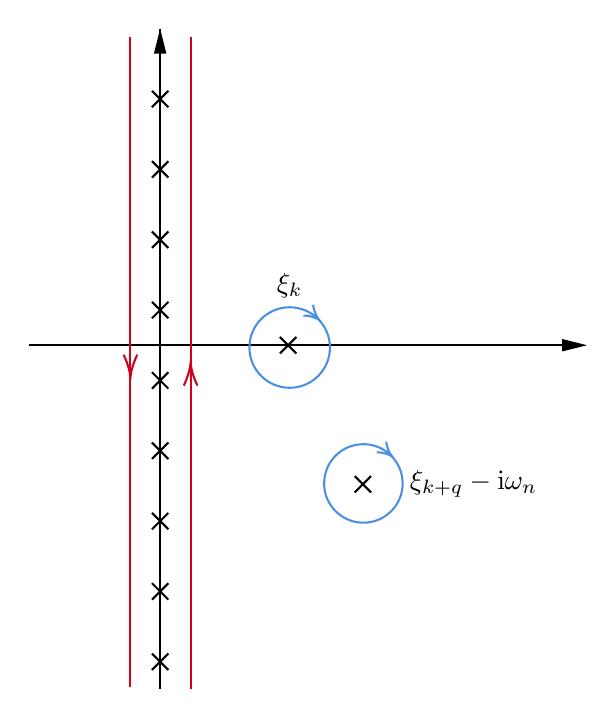
\begin{tikzpicture}[x=0.75pt,y=0.75pt,yscale=-1,xscale=1]
%uncomment if require: \path (0,379); %set diagram left start at 0, and has height of 379

%Straight Lines [id:da4696139814770115] 
\draw [color={rgb, 255:red, 208; green, 2; blue, 27 }  ,draw opacity=1 ]   (275,21.67) -- (275,334.67) ;
%Straight Lines [id:da08437675696747471] 
\draw    (226,170.17) -- (493,170.17) ;
\draw [shift={(495,170.17)}, rotate = 180] [fill={rgb, 255:red, 0; green, 0; blue, 0 }  ][line width=0.08]  [draw opacity=0] (12,-3) -- (0,0) -- (12,3) -- cycle    ;
%Straight Lines [id:da3198194636768519] 
\draw    (289.33,335.67) -- (289.33,19.67) ;
\draw [shift={(289.33,17.67)}, rotate = 450] [fill={rgb, 255:red, 0; green, 0; blue, 0 }  ][line width=0.08]  [draw opacity=0] (12,-3) -- (0,0) -- (12,3) -- cycle    ;
%Straight Lines [id:da33911829063354104] 
\draw    (289.33,17.67) -- (289.33,51.56) ;
\draw [shift={(289.33,51.56)}, rotate = 135] [color={rgb, 255:red, 0; green, 0; blue, 0 }  ][line width=0.75]    (-5.59,0) -- (5.59,0)(0,5.59) -- (0,-5.59)   ;
%Straight Lines [id:da9683910595635019] 
\draw    (289.33,51.56) -- (289.33,85.44) ;
\draw [shift={(289.33,85.44)}, rotate = 135] [color={rgb, 255:red, 0; green, 0; blue, 0 }  ][line width=0.75]    (-5.59,0) -- (5.59,0)(0,5.59) -- (0,-5.59)   ;
%Straight Lines [id:da23125512620723487] 
\draw    (289.33,85.44) -- (289.33,119.33) ;
\draw [shift={(289.33,119.33)}, rotate = 135] [color={rgb, 255:red, 0; green, 0; blue, 0 }  ][line width=0.75]    (-5.59,0) -- (5.59,0)(0,5.59) -- (0,-5.59)   ;
%Straight Lines [id:da9012438256404278] 
\draw    (289.33,119.33) -- (289.33,153.22) ;
\draw [shift={(289.33,153.22)}, rotate = 135] [color={rgb, 255:red, 0; green, 0; blue, 0 }  ][line width=0.75]    (-5.59,0) -- (5.59,0)(0,5.59) -- (0,-5.59)   ;
%Straight Lines [id:da9577216099300172] 
\draw    (289.33,153.22) -- (289.33,187.11) ;
\draw [shift={(289.33,187.11)}, rotate = 135] [color={rgb, 255:red, 0; green, 0; blue, 0 }  ][line width=0.75]    (-5.59,0) -- (5.59,0)(0,5.59) -- (0,-5.59)   ;
%Straight Lines [id:da12515690343677166] 
\draw    (289.33,187.11) -- (289.33,221) ;
\draw [shift={(289.33,221)}, rotate = 135] [color={rgb, 255:red, 0; green, 0; blue, 0 }  ][line width=0.75]    (-5.59,0) -- (5.59,0)(0,5.59) -- (0,-5.59)   ;
%Straight Lines [id:da5860572173856167] 
\draw    (289.33,221) -- (289.33,254.89) ;
\draw [shift={(289.33,254.89)}, rotate = 135] [color={rgb, 255:red, 0; green, 0; blue, 0 }  ][line width=0.75]    (-5.59,0) -- (5.59,0)(0,5.59) -- (0,-5.59)   ;
%Straight Lines [id:da2632609556473693] 
\draw    (289.33,254.89) -- (289.33,288.78) ;
\draw [shift={(289.33,288.78)}, rotate = 135] [color={rgb, 255:red, 0; green, 0; blue, 0 }  ][line width=0.75]    (-5.59,0) -- (5.59,0)(0,5.59) -- (0,-5.59)   ;
%Straight Lines [id:da5620983068494032] 
\draw    (289.33,288.78) -- (289.33,322.67) ;
\draw [shift={(289.33,322.67)}, rotate = 135] [color={rgb, 255:red, 0; green, 0; blue, 0 }  ][line width=0.75]    (-5.59,0) -- (5.59,0)(0,5.59) -- (0,-5.59)   ;
%Straight Lines [id:da21282805052989584] 
\draw    (230,170.17) -- (351,170.17) ;
\draw [shift={(351,170.17)}, rotate = 45] [color={rgb, 255:red, 0; green, 0; blue, 0 }  ][line width=0.75]    (-5.59,0) -- (5.59,0)(0,5.59) -- (0,-5.59)   ;
%Straight Lines [id:da0020189550089222408] 
\draw    (387,237.17) ;
\draw [shift={(387,237.17)}, rotate = 45] [color={rgb, 255:red, 0; green, 0; blue, 0 }  ][line width=0.75]    (-5.59,0) -- (5.59,0)(0,5.59) -- (0,-5.59)   ;
%Straight Lines [id:da27901434379198053] 
\draw [color={rgb, 255:red, 208; green, 2; blue, 27 }  ,draw opacity=1 ]   (304,335.67) -- (304,21.67) ;
\draw [shift={(304,178.67)}, rotate = 450] [color={rgb, 255:red, 208; green, 2; blue, 27 }  ,draw opacity=1 ][line width=0.75]    (10.93,-3.29) .. controls (6.95,-1.4) and (3.31,-0.3) .. (0,0) .. controls (3.31,0.3) and (6.95,1.4) .. (10.93,3.29)   ;
%Straight Lines [id:da7266322759719097] 
\draw [color={rgb, 255:red, 208; green, 2; blue, 27 }  ,draw opacity=1 ]   (275,36.67) -- (275,334.67) ;
\draw [shift={(275,185.67)}, rotate = 270] [color={rgb, 255:red, 208; green, 2; blue, 27 }  ,draw opacity=1 ][line width=0.75]    (10.93,-3.29) .. controls (6.95,-1.4) and (3.31,-0.3) .. (0,0) .. controls (3.31,0.3) and (6.95,1.4) .. (10.93,3.29)   ;
%Shape: Ellipse [id:dp2554624294784811] 
\draw  [color={rgb, 255:red, 74; green, 144; blue, 226 }  ,draw opacity=1 ] (332.33,171.27) .. controls (332.33,160.55) and (341.02,151.87) .. (351.73,151.87) .. controls (362.45,151.87) and (371.13,160.55) .. (371.13,171.27) .. controls (371.13,181.98) and (362.45,190.67) .. (351.73,190.67) .. controls (341.02,190.67) and (332.33,181.98) .. (332.33,171.27) -- cycle ;
\draw  [color={rgb, 255:red, 74; green, 144; blue, 226 }  ,draw opacity=1 ] (362.99,150.67) .. controls (363.43,153.65) and (364.39,156.05) .. (365.85,157.88) .. controls (363.87,156.62) and (361.38,155.95) .. (358.36,155.84) ;

%Shape: Ellipse [id:dp2358273364781196] 
\draw  [color={rgb, 255:red, 74; green, 144; blue, 226 }  ,draw opacity=1 ] (368.33,236.75) .. controls (368.33,226.3) and (376.8,217.84) .. (387.25,217.84) .. controls (397.7,217.84) and (406.16,226.3) .. (406.16,236.75) .. controls (406.16,247.2) and (397.7,255.67) .. (387.25,255.67) .. controls (376.8,255.67) and (368.33,247.2) .. (368.33,236.75) -- cycle ;
\draw  [color={rgb, 255:red, 74; green, 144; blue, 226 }  ,draw opacity=1 ] (398.23,216.67) .. controls (398.65,219.57) and (399.58,221.92) .. (401.02,223.7) .. controls (399.08,222.48) and (396.65,221.81) .. (393.71,221.71) ;


% Text Node
\draw (351.73,148.87) node [anchor=south] [inner sep=0.75pt]    {$\xi _{\boldsymbol{k}}$};
% Text Node
\draw (408.16,236.75) node [anchor=west] [inner sep=0.75pt]    {$\xi _{\boldsymbol{k} +\boldsymbol{q}} -\mathrm{i} \omega _{n}$};

\end{tikzpicture}
    \caption{$f(z) \frac{1}{z - \zeta_{\vb*{k}}} \frac{1}{z + \ii \omega_n - \xi_{\vb*{k} + \vb*{q}}}$在复平面上的解析结构}
    \label{fig:rpa-pole}
\end{figure}

\eqref{eq:ext-electron-retarded-green-function}可以推导出托马斯-费米屏蔽。
在$V_\text{eff}$在时间和空间上都变化非常缓慢时,只需要考虑$\vb*{q}$接近零的那部分傅里叶分量。
让$\omega$和$\vb*{q}$趋于零,我们有
\[
    G_{nn}^\text{ret, 0}(\vb*{q}, \ii \omega_n) = 2 \sum_{\vb*{k}} \dv{f(\xi_{\vb*{k}})}{\xi_{\vb*{k}}} = - 2 \sum_{\vb*{k}} \dv{f(\xi_{\vb*{k}})}{\mu} = - \pdv{n}{\mu} = - N(0),
\]
这正是我们在托马斯-费米屏蔽中做的近似:这表明RPA近似在低频下的确和托马斯-费米屏蔽一致,正如我们之前说明的那样。

\subsection{等离子体和等离激元}

考虑$\omega$非常高的极限,此时做展开
\[
    \frac{1}{\omega + \xi_{\vb*{k}} - \xi_{\vb*{k} + \vb*{q}} + \ii 0^+} = \frac{1}{\omega} - \frac{\xi_{\vb*{k}} - \xi_{\vb*{k} + \vb*{q}}}{\omega^2} + \cdots,
\]
展开到前两阶,代入\eqref{eq:ext-electron-retarded-green-function},得到
\[
    \begin{aligned}
        G_{nn}^\text{ret, 0}(\vb*{q}, \ii \omega_n) &= - \frac{2}{\omega^2} \sum_{\vb*{k}} (f(\xi_{\vb*{k}}) - f(\xi_{\vb*{k} + \vb*{q}})) (\xi_{\vb*{k}} - \xi_{\vb*{k} + \vb*{q}}) \\
        &= \frac{2 q^2}{m \omega^2} \sum_{\vb*{k}} f(\xi_{\vb*{k}}), 
    \end{aligned}
\]
于是就得到
\begin{equation}
    G_{nn}^\text{ret, 0}(\vb*{q}, \ii \omega_n) = \frac{q^2 n_\text{e}}{m \omega^2},
\end{equation}
相应的,
\[
    \epsilon(\vb*{k}, \omega \to 0) = 1 - \frac{4 \pi e^2 n_\text{e}}{m \omega^2},
\]
定义
\begin{equation}
    \omega_\text{p}^2 = \frac{4 \pi e^2 n_\text{e}}{m},
\end{equation}
就得到
\begin{equation}
    \epsilon(\vb*{k}, \omega \to 0) = 1 - \frac{\omega_\text{p}^2}{\omega^2}.
\end{equation}
考虑到\eqref{eq:ext-electron-ret-nn},当$\omega = \omega_\text{p}$时格林函数出现奇点,即此处有集体激发。
$G^\text{ret}_{nn}(\vb*{k}, \omega)$是一个密度-密度格林函数,对任意的动量,在$\omega = \omega_\text{p}$处都有一个密度波的集体激发模式。
我们此处的计算是在频率非常大,以至于介质几乎是等离子体时得到的,因此这种集体激发实际上正是\concept{等离激元}。
物理地看,等离激元是密度波这件事实际上说明了等离子体中的电子运动方式,即一个电子和一个空穴成对地振荡。
这个集体激发的频谱是平的,这当然是因为我们假定光速无穷大,完全使用库伦相互作用。如果考虑到光速有限,使用麦克斯韦方程可以推出
\begin{equation}
    \omega_{\vb*{k}}^2 = \omega_\text{p}^2 + c^2 k^2 / \epsilon(\infty),
\end{equation}
即光子的一个模式和固体发生耦合,打开了一个能隙。在假定光速无限时,丢弃不可见、恒定的无穷大项(相当于将元激发的产生湮灭算符的时间演化加上一个因子$\ee^{\ii c k t}$)就得到
\[
    \omega_{\vb*{k}} = \omega_\text{p},
\]
即我们算出的结果。

\section{凝胶模型}

\begin{figure}
    \centering
    

\tikzset{every picture/.style={line width=0.75pt}} %set default line width to 0.75pt        

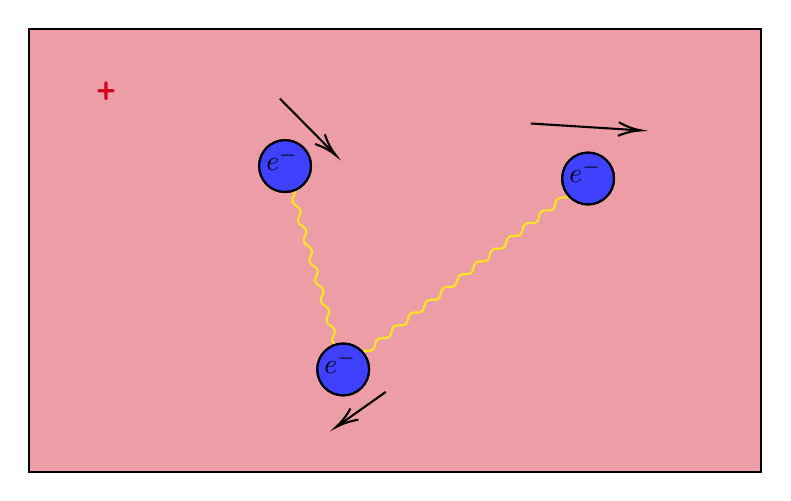
\begin{tikzpicture}[x=0.75pt,y=0.75pt,yscale=-1,xscale=1]
%uncomment if require: \path (0,300); %set diagram left start at 0, and has height of 300

%Shape: Rectangle [id:dp047247226295811684] 
\draw  [fill={rgb, 255:red, 208; green, 2; blue, 27 }  ,fill opacity=0.39 ] (124,18.33) -- (477,18.33) -- (477,232) -- (124,232) -- cycle ;
%Straight Lines [id:da1214980139749513] 
\draw [color={rgb, 255:red, 248; green, 231; blue, 28 }  ,draw opacity=1 ]   (393.5,90.5) .. controls (393.21,92.84) and (391.9,93.86) .. (389.56,93.57) .. controls (387.22,93.28) and (385.9,94.31) .. (385.61,96.65) .. controls (385.32,98.99) and (384.01,100.01) .. (381.67,99.72) .. controls (379.33,99.43) and (378.02,100.46) .. (377.73,102.8) .. controls (377.44,105.14) and (376.12,106.16) .. (373.78,105.87) .. controls (371.44,105.58) and (370.13,106.61) .. (369.84,108.95) .. controls (369.55,111.29) and (368.24,112.31) .. (365.9,112.02) .. controls (363.56,111.73) and (362.24,112.75) .. (361.95,115.09) .. controls (361.66,117.43) and (360.35,118.46) .. (358.01,118.17) .. controls (355.67,117.88) and (354.36,118.9) .. (354.07,121.24) .. controls (353.78,123.58) and (352.47,124.61) .. (350.13,124.32) .. controls (347.79,124.03) and (346.47,125.05) .. (346.18,127.39) .. controls (345.89,129.73) and (344.58,130.76) .. (342.24,130.47) .. controls (339.9,130.18) and (338.59,131.2) .. (338.3,133.54) .. controls (338.01,135.88) and (336.69,136.9) .. (334.35,136.61) .. controls (332.01,136.32) and (330.7,137.35) .. (330.41,139.69) .. controls (330.12,142.03) and (328.81,143.05) .. (326.47,142.76) .. controls (324.13,142.47) and (322.81,143.5) .. (322.52,145.84) .. controls (322.23,148.18) and (320.92,149.2) .. (318.58,148.91) .. controls (316.24,148.62) and (314.93,149.65) .. (314.64,151.99) .. controls (314.35,154.33) and (313.03,155.35) .. (310.69,155.06) .. controls (308.35,154.77) and (307.04,155.8) .. (306.75,158.14) .. controls (306.46,160.48) and (305.15,161.5) .. (302.81,161.21) .. controls (300.47,160.92) and (299.15,161.94) .. (298.86,164.28) .. controls (298.57,166.62) and (297.26,167.65) .. (294.92,167.36) .. controls (292.58,167.07) and (291.27,168.09) .. (290.98,170.43) .. controls (290.69,172.77) and (289.37,173.8) .. (287.03,173.51) .. controls (284.69,173.22) and (283.38,174.24) .. (283.09,176.58) .. controls (282.8,178.92) and (281.49,179.95) .. (279.15,179.66) -- (275.5,182.5) -- (275.5,182.5) ;
%Straight Lines [id:da28890006353055053] 
\draw [color={rgb, 255:red, 248; green, 231; blue, 28 }  ,draw opacity=1 ]   (247.5,84.5) .. controls (249.56,85.65) and (250.02,87.25) .. (248.87,89.31) .. controls (247.73,91.37) and (248.19,92.97) .. (250.25,94.12) .. controls (252.31,95.26) and (252.77,96.86) .. (251.62,98.92) .. controls (250.47,100.98) and (250.93,102.58) .. (252.99,103.73) .. controls (255.05,104.88) and (255.51,106.48) .. (254.37,108.54) .. controls (253.22,110.6) and (253.68,112.2) .. (255.74,113.35) .. controls (257.8,114.49) and (258.26,116.09) .. (257.12,118.15) .. controls (255.97,120.21) and (256.43,121.81) .. (258.49,122.96) .. controls (260.55,124.11) and (261.01,125.71) .. (259.86,127.77) .. controls (258.72,129.83) and (259.18,131.43) .. (261.24,132.58) .. controls (263.3,133.72) and (263.76,135.32) .. (262.61,137.38) .. controls (261.46,139.44) and (261.92,141.04) .. (263.98,142.19) .. controls (266.04,143.34) and (266.5,144.94) .. (265.36,147) .. controls (264.21,149.06) and (264.67,150.66) .. (266.73,151.81) .. controls (268.79,152.95) and (269.25,154.55) .. (268.1,156.61) .. controls (266.96,158.67) and (267.42,160.27) .. (269.48,161.42) .. controls (271.54,162.57) and (272,164.17) .. (270.85,166.23) .. controls (269.7,168.29) and (270.16,169.89) .. (272.22,171.04) .. controls (274.28,172.18) and (274.74,173.78) .. (273.6,175.84) .. controls (272.45,177.9) and (272.91,179.5) .. (274.97,180.65) -- (275.5,182.5) -- (275.5,182.5) ;
%Shape: Circle [id:dp8134342150548997] 
\draw  [fill={rgb, 255:red, 255; green, 255; blue, 255 }  ,fill opacity=1 ] (235,84.5) .. controls (235,77.6) and (240.6,72) .. (247.5,72) .. controls (254.4,72) and (260,77.6) .. (260,84.5) .. controls (260,91.4) and (254.4,97) .. (247.5,97) .. controls (240.6,97) and (235,91.4) .. (235,84.5) -- cycle ;
%Shape: Circle [id:dp8710949772350924] 
\draw  [fill={rgb, 255:red, 0; green, 0; blue, 255 }  ,fill opacity=0.75 ] (235,84.5) .. controls (235,77.6) and (240.6,72) .. (247.5,72) .. controls (254.4,72) and (260,77.6) .. (260,84.5) .. controls (260,91.4) and (254.4,97) .. (247.5,97) .. controls (240.6,97) and (235,91.4) .. (235,84.5) -- cycle ;


%Shape: Circle [id:dp7228108183537771] 
\draw  [fill={rgb, 255:red, 255; green, 255; blue, 255 }  ,fill opacity=1 ] (381,90.5) .. controls (381,83.6) and (386.6,78) .. (393.5,78) .. controls (400.4,78) and (406,83.6) .. (406,90.5) .. controls (406,97.4) and (400.4,103) .. (393.5,103) .. controls (386.6,103) and (381,97.4) .. (381,90.5) -- cycle ;
%Shape: Circle [id:dp8018452416730255] 
\draw  [fill={rgb, 255:red, 0; green, 0; blue, 255 }  ,fill opacity=0.75 ] (381,90.5) .. controls (381,83.6) and (386.6,78) .. (393.5,78) .. controls (400.4,78) and (406,83.6) .. (406,90.5) .. controls (406,97.4) and (400.4,103) .. (393.5,103) .. controls (386.6,103) and (381,97.4) .. (381,90.5) -- cycle ;


%Shape: Circle [id:dp03452463129100414] 
\draw  [fill={rgb, 255:red, 255; green, 255; blue, 255 }  ,fill opacity=1 ] (263,182.5) .. controls (263,175.6) and (268.6,170) .. (275.5,170) .. controls (282.4,170) and (288,175.6) .. (288,182.5) .. controls (288,189.4) and (282.4,195) .. (275.5,195) .. controls (268.6,195) and (263,189.4) .. (263,182.5) -- cycle ;
%Shape: Circle [id:dp18588186480919022] 
\draw  [fill={rgb, 255:red, 0; green, 0; blue, 255 }  ,fill opacity=0.75 ] (263,182.5) .. controls (263,175.6) and (268.6,170) .. (275.5,170) .. controls (282.4,170) and (288,175.6) .. (288,182.5) .. controls (288,189.4) and (282.4,195) .. (275.5,195) .. controls (268.6,195) and (263,189.4) .. (263,182.5) -- cycle ;


%Straight Lines [id:da3558568035781704] 
\draw    (245,52) -- (270.59,77.91) ;
\draw [shift={(272,79.33)}, rotate = 225.35] [color={rgb, 255:red, 0; green, 0; blue, 0 }  ][line width=0.75]    (10.93,-3.29) .. controls (6.95,-1.4) and (3.31,-0.3) .. (0,0) .. controls (3.31,0.3) and (6.95,1.4) .. (10.93,3.29)   ;
%Straight Lines [id:da8712247783624321] 
\draw    (366,64) -- (417,67.21) ;
\draw [shift={(419,67.33)}, rotate = 183.6] [color={rgb, 255:red, 0; green, 0; blue, 0 }  ][line width=0.75]    (10.93,-3.29) .. controls (6.95,-1.4) and (3.31,-0.3) .. (0,0) .. controls (3.31,0.3) and (6.95,1.4) .. (10.93,3.29)   ;
%Straight Lines [id:da5825968843197606] 
\draw    (296,193.33) -- (273.63,209.18) ;
\draw [shift={(272,210.33)}, rotate = 324.69] [color={rgb, 255:red, 0; green, 0; blue, 0 }  ][line width=0.75]    (10.93,-3.29) .. controls (6.95,-1.4) and (3.31,-0.3) .. (0,0) .. controls (3.31,0.3) and (6.95,1.4) .. (10.93,3.29)   ;

% Text Node
\draw (155,44) node [anchor=north west][inner sep=0.75pt]  [color={rgb, 255:red, 208; green, 2; blue, 27 }  ,opacity=1 ] [align=left] {{\fontfamily{pcr}\selectfont \textbf{{\large +}}}};
% Text Node
\draw (237,74.4) node [anchor=north west][inner sep=0.75pt]    {$\textcolor[rgb]{0,0,0}{e^{-}}$};
% Text Node
\draw (383,80.4) node [anchor=north west][inner sep=0.75pt]    {$\textcolor[rgb]{0,0,0}{e}\textcolor[rgb]{0,0,0}{^{-}}$};
% Text Node
\draw (265,172.4) node [anchor=north west][inner sep=0.75pt]    {$\textcolor[rgb]{0,0,0}{e}\textcolor[rgb]{0,0,0}{^{-}}$};


\end{tikzpicture}

    \caption{凝胶模型:原子实带来均一的、实际上不会对约束在晶体中的电子产生任何影响的正电荷背景,主要的物理是电子以及它们的电磁相互作用}
\end{figure}

以上所有的处理相互作用的做法都有浓重的半经典色彩,从本节开始我们在场论框架下比较系统地做计算。
本节讨论\concept{凝胶模型},这是一种将库伦散射不做任何处理地当成微扰,并且将金属中的原子当成均匀的正电荷凝胶的金属模型。
前一个假设——微扰论适用——实际上冒了很大风险,但是的确有一定实验证据支持它,因为实验上金属和近独立电子气的行为确实很相似;对这件事的进一步利用见\autoref{sec:landau-fermi-liquid}。
后一个假设对那些在其中的电子很像自由电子的金属系统是确实成立的,因为这样的系统中晶格对电子的作用比较小,从而能量微扰可以只考虑最低阶的\eqref{eq:first-order-energy-perturbation},其物理直观就是均匀的正电荷凝胶,它让所有电子的能量整体上升或是下降了一定量。
我们把这部分能量变化整体归入化学势。

因此,到最后,所谓凝胶模型实际上就是在讨论自由电子加上可以微扰处理的库仑相互作用之后会发生什么。

\subsection{费曼规则}

我们在虚时间场论和倒空间(即$(\omega, \vb*{k})$,其中$\vb*{k}$是简约波矢)下工作,则费曼规则为:
\begin{itemize}
    \item 传播子为\begin{equation}
    \begin{gathered}
        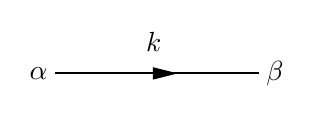
\begin{tikzpicture}[x=0.75pt,y=0.75pt,yscale=-1,xscale=1]
            %uncomment if require: \path (0,300); %set diagram left start at 0, and has height of 300
            
            %Straight Lines [id:da865326669998641] 
            \draw    (84,141.93) -- (136.7,141.93) ;
            \draw [shift={(138.7,141.93)}, rotate = 180] [fill={rgb, 255:red, 0; green, 0; blue, 0 }  ][line width=0.08]  [draw opacity=0] (12,-3) -- (0,0) -- (12,3) -- cycle    ;
            %Straight Lines [id:da20498887952582923] 
            \draw    (79.46,141.93) -- (177.93,141.93) ;
            
            % Text Node
            \draw (77.46,141.93) node [anchor=east] [inner sep=0.75pt]    {$\alpha $};
            % Text Node
            \draw (179.93,141.93) node [anchor=west] [inner sep=0.75pt]    {$\beta $};
            % Text Node
            \draw (122,120.4) node [anchor=north west][inner sep=0.75pt]    {$\boldsymbol{k}$};
            
            
            \end{tikzpicture}                
    \end{gathered} = - \frac{\delta_{\alpha \beta}}{\ii \omega_n - \xi_{\vb*{k}}},
\end{equation}
    其中
    \begin{equation}
        \xi_{\vb*{k}} = \frac{\vb*{k}^2}{2m} - \mu
    \end{equation}
    \item 相互作用使用(为了节约符号,有时候我们会将$(\vb*{q}, \omega_n)$这样的四元组简写为$q$,其中$\omega_n = p^0$。)\begin{equation}
    \begin{gathered}
        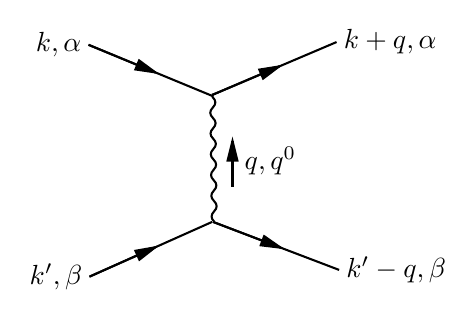
\begin{tikzpicture}[x=0.75pt,y=0.75pt,yscale=-1,xscale=1]
            %Straight Lines [id:da15915538235750892] 
            \draw    (100.17,172.51) -- (131.95,158.32) ;
            \draw [shift={(133.77,157.5)}, rotate = 515.9300000000001] [fill={rgb, 255:red, 0; green, 0; blue, 0 }  ][line width=0.08]  [draw opacity=0] (12,-3) -- (0,0) -- (12,3) -- cycle    ;
            %Straight Lines [id:da595892295722313] 
            \draw    (100.17,172.51) -- (159.26,146.12) ;
            
            %Straight Lines [id:da41375516068648066] 
            \draw    (160.29,146.04) .. controls (158.6,144.39) and (158.57,142.73) .. (160.22,141.04) .. controls (161.87,139.35) and (161.85,137.69) .. (160.16,136.04) .. controls (158.47,134.39) and (158.45,132.73) .. (160.1,131.04) .. controls (161.74,129.35) and (161.72,127.69) .. (160.03,126.04) .. controls (158.34,124.39) and (158.32,122.73) .. (159.97,121.04) .. controls (161.62,119.35) and (161.6,117.69) .. (159.91,116.04) .. controls (158.22,114.39) and (158.2,112.73) .. (159.84,111.04) .. controls (161.49,109.35) and (161.47,107.69) .. (159.78,106.04) .. controls (158.09,104.39) and (158.07,102.73) .. (159.72,101.04) .. controls (161.36,99.35) and (161.34,97.69) .. (159.65,96.04) .. controls (157.96,94.39) and (157.94,92.73) .. (159.59,91.04) .. controls (161.24,89.35) and (161.22,87.69) .. (159.53,86.04) -- (159.51,84.35) -- (159.51,84.35) ;
            %Straight Lines [id:da18427908684914152] 
            \draw    (159.7,146.12) -- (192.38,158.57) ;
            \draw [shift={(194.25,159.28)}, rotate = 200.85] [fill={rgb, 255:red, 0; green, 0; blue, 0 }  ][line width=0.08]  [draw opacity=0] (12,-3) -- (0,0) -- (12,3) -- cycle    ;
            %Straight Lines [id:da5517253733622631] 
            \draw    (159.7,146.12) -- (220.46,169.26) ;
            
            %Straight Lines [id:da9982758254698763] 
            \draw    (99.72,60.8) -- (131.97,74.12) ;
            \draw [shift={(133.82,74.88)}, rotate = 202.44] [fill={rgb, 255:red, 0; green, 0; blue, 0 }  ][line width=0.08]  [draw opacity=0] (12,-3) -- (0,0) -- (12,3) -- cycle    ;
            %Straight Lines [id:da26812450354509565] 
            \draw    (99.72,60.8) -- (159.69,85.57) ;
            
            %Straight Lines [id:da1756933542309722] 
            \draw    (159.57,84.84) -- (191.65,71.2) ;
            \draw [shift={(193.49,70.41)}, rotate = 516.96] [fill={rgb, 255:red, 0; green, 0; blue, 0 }  ][line width=0.08]  [draw opacity=0] (12,-3) -- (0,0) -- (12,3) -- cycle    ;
            %Straight Lines [id:da7638586957076614] 
            \draw    (159.57,84.84) -- (219.22,59.47) ;
            
            %Straight Lines [id:da9798265876333652] 
            \draw    (169.09,129.1) -- (169.09,107.04) ;
            \draw [shift={(169.09,105.04)}, rotate = 450] [fill={rgb, 255:red, 0; green, 0; blue, 0 }  ][line width=0.08]  [draw opacity=0] (12,-3) -- (0,0) -- (12,3) -- cycle    ;
            
            % Text Node
            \draw (97.72,60.8) node [anchor=east] [inner sep=0.75pt]    {$\boldsymbol{k} ,\alpha $};
            % Text Node
            \draw (221.22,59.47) node [anchor=west] [inner sep=0.75pt]    {$\boldsymbol{k} +\boldsymbol{q} ,\alpha $};
            % Text Node
            \draw (173.48,108.5) node [anchor=north west][inner sep=0.75pt]    {$\boldsymbol{q}, \ii q^0$};
            % Text Node
            \draw (98.17,172.51) node [anchor=east] [inner sep=0.75pt]    {$\boldsymbol{k} ',\beta $};
            % Text Node
            \draw (222.46,169.26) node [anchor=west] [inner sep=0.75pt]    {$\boldsymbol{k} '-\boldsymbol{q} ,\beta $};
            \end{tikzpicture}
    \end{gathered} = \frac{1}{V} \frac{4\pi e^2}{\abs*{\vb*{q}}^2},
\end{equation}
    表示,其中$\vb*{q}$可以随意取值(见\autoref{sec:interaction-bloch})。
    需要对$\vb*{q}$做求和,并注意由于库仑相互作用被假定为瞬时发生的,光子频率$\ii q^0$始终是零。
    光子由于已经被积掉了,不贡献传播子。可以将\eqref{eq:jellium-vertex}整体看成一个给出库仑相互作用势能的顶角,不过更常见的做法是将光子线称为\concept{相互作用线},将相互作用线和电子线的连接点称为顶角。
    两个顶角被一条相互作用线连接则贡献一个库伦相互作用势能。
    通常系统均足够大,此时有\begin{equation}
    \begin{gathered}
        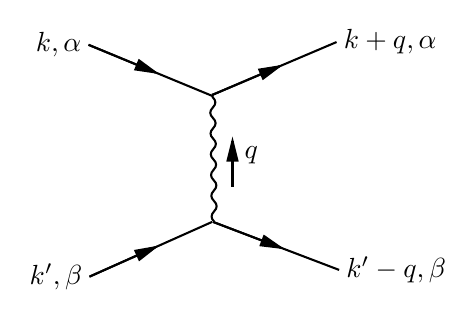
\begin{tikzpicture}[x=0.75pt,y=0.75pt,yscale=-1,xscale=1]
            %Straight Lines [id:da15915538235750892] 
            \draw    (100.17,172.51) -- (131.95,158.32) ;
            \draw [shift={(133.77,157.5)}, rotate = 515.9300000000001] [fill={rgb, 255:red, 0; green, 0; blue, 0 }  ][line width=0.08]  [draw opacity=0] (12,-3) -- (0,0) -- (12,3) -- cycle    ;
            %Straight Lines [id:da595892295722313] 
            \draw    (100.17,172.51) -- (159.26,146.12) ;
            
            %Straight Lines [id:da41375516068648066] 
            \draw    (160.29,146.04) .. controls (158.6,144.39) and (158.57,142.73) .. (160.22,141.04) .. controls (161.87,139.35) and (161.85,137.69) .. (160.16,136.04) .. controls (158.47,134.39) and (158.45,132.73) .. (160.1,131.04) .. controls (161.74,129.35) and (161.72,127.69) .. (160.03,126.04) .. controls (158.34,124.39) and (158.32,122.73) .. (159.97,121.04) .. controls (161.62,119.35) and (161.6,117.69) .. (159.91,116.04) .. controls (158.22,114.39) and (158.2,112.73) .. (159.84,111.04) .. controls (161.49,109.35) and (161.47,107.69) .. (159.78,106.04) .. controls (158.09,104.39) and (158.07,102.73) .. (159.72,101.04) .. controls (161.36,99.35) and (161.34,97.69) .. (159.65,96.04) .. controls (157.96,94.39) and (157.94,92.73) .. (159.59,91.04) .. controls (161.24,89.35) and (161.22,87.69) .. (159.53,86.04) -- (159.51,84.35) -- (159.51,84.35) ;
            %Straight Lines [id:da18427908684914152] 
            \draw    (159.7,146.12) -- (192.38,158.57) ;
            \draw [shift={(194.25,159.28)}, rotate = 200.85] [fill={rgb, 255:red, 0; green, 0; blue, 0 }  ][line width=0.08]  [draw opacity=0] (12,-3) -- (0,0) -- (12,3) -- cycle    ;
            %Straight Lines [id:da5517253733622631] 
            \draw    (159.7,146.12) -- (220.46,169.26) ;
            
            %Straight Lines [id:da9982758254698763] 
            \draw    (99.72,60.8) -- (131.97,74.12) ;
            \draw [shift={(133.82,74.88)}, rotate = 202.44] [fill={rgb, 255:red, 0; green, 0; blue, 0 }  ][line width=0.08]  [draw opacity=0] (12,-3) -- (0,0) -- (12,3) -- cycle    ;
            %Straight Lines [id:da26812450354509565] 
            \draw    (99.72,60.8) -- (159.69,85.57) ;
            
            %Straight Lines [id:da1756933542309722] 
            \draw    (159.57,84.84) -- (191.65,71.2) ;
            \draw [shift={(193.49,70.41)}, rotate = 516.96] [fill={rgb, 255:red, 0; green, 0; blue, 0 }  ][line width=0.08]  [draw opacity=0] (12,-3) -- (0,0) -- (12,3) -- cycle    ;
            %Straight Lines [id:da7638586957076614] 
            \draw    (159.57,84.84) -- (219.22,59.47) ;
            
            %Straight Lines [id:da9798265876333652] 
            \draw    (169.09,129.1) -- (169.09,107.04) ;
            \draw [shift={(169.09,105.04)}, rotate = 450] [fill={rgb, 255:red, 0; green, 0; blue, 0 }  ][line width=0.08]  [draw opacity=0] (12,-3) -- (0,0) -- (12,3) -- cycle    ;
            
            % Text Node
            \draw (97.72,60.8) node [anchor=east] [inner sep=0.75pt]    {$\boldsymbol{k} ,\alpha $};
            % Text Node
            \draw (221.22,59.47) node [anchor=west] [inner sep=0.75pt]    {$\boldsymbol{k} +\boldsymbol{q} ,\alpha $};
            % Text Node
            \draw (173.48,108.5) node [anchor=north west][inner sep=0.75pt]    {$\boldsymbol{q}$};
            % Text Node
            \draw (98.17,172.51) node [anchor=east] [inner sep=0.75pt]    {$\boldsymbol{k} ',\beta $};
            % Text Node
            \draw (222.46,169.26) node [anchor=west] [inner sep=0.75pt]    {$\boldsymbol{k} '-\boldsymbol{q} ,\beta $};
            \end{tikzpicture}
    \end{gathered} = \frac{1}{\beta} \sum_{\omega_n} \int \frac{\dd[3]{\vb*{q}}}{(2\pi)^3} \frac{4\pi e^2}{\abs*{\vb*{q}}^2}.
\end{equation}
    \item 闭合电子回线需要乘上$-1$。
\end{itemize}
不要忘记按照松原格林函数的定义,将需要计算的所有图求和后需要加上负号才能够得到松原格林函数。

我们仍然使用波浪线表示库仑相互作用,表示这是光子介导的。在之后的模型中,相互作用势会被多次修正,得到一个形式复杂的,\eqref{eq:general-electron-electron-interaction}形式的理论,那时将使用虚线表示电子间排斥。

\subsection{正规自能计算和Hartree-Fock近似}

\begin{back}{单粒子格林函数的自能修正}{self-energy}
    做自能计算时我们有
    \[
        \frac{1}{\begin{gathered}
            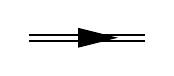
\begin{tikzpicture}[x=0.75pt,y=0.75pt,yscale=-1,xscale=1]
                %uncomment if require: \path (0,300); %set diagram left start at 0, and has height of 300
                
                %Straight Lines [id:da1745692111058319] 
                \draw    (186.35,103.5) -- (235.71,103.5)(186.35,106.5) -- (235.71,106.5) ;
                %Straight Lines [id:da12764386282624862] 
                \draw    (179.71,103.5) -- (214.71,103.5)(179.71,106.5) -- (214.71,106.5) ;
                \draw [shift={(222.71,105)}, rotate = 180] [fill={rgb, 255:red, 0; green, 0; blue, 0 }  ][line width=0.08]  [draw opacity=0] (19.2,-4.8) -- (0,0) -- (19.2,4.8) -- cycle    ;
                \end{tikzpicture}            
        \end{gathered}} = 
        \frac{1}{\begin{gathered}
            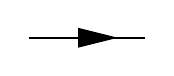
\begin{tikzpicture}[x=0.75pt,y=0.75pt,yscale=-1,xscale=1]
                %uncomment if require: \path (0,300); %set diagram left start at 0, and has height of 300
                
                %Straight Lines [id:da1745692111058319] 
                \draw    (186.35,105) -- (235.71,105) ;
                %Straight Lines [id:da12764386282624862] 
                \draw    (179.71,105) -- (220.71,105) ;
                \draw [shift={(222.71,105)}, rotate = 180] [fill={rgb, 255:red, 0; green, 0; blue, 0 }  ][line width=0.08]  [draw opacity=0] (19.2,-4.8) -- (0,0) -- (19.2,4.8) -- cycle    ;
                \end{tikzpicture}
        \end{gathered}} - \begin{gathered}
            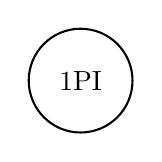
\begin{tikzpicture}[x=0.75pt,y=0.75pt,yscale=-1,xscale=1]
                %uncomment if require: \path (0,300); %set diagram left start at 0, and has height of 300
                
                %Shape: Circle [id:dp8588117224452179] 
                \draw   (100,144) .. controls (100,130.19) and (111.19,119) .. (125,119) .. controls (138.81,119) and (150,130.19) .. (150,144) .. controls (150,157.81) and (138.81,169) .. (125,169) .. controls (111.19,169) and (100,157.81) .. (100,144) -- cycle ;
                
                % Text Node
                \draw (125,144) node   [align=left] {1PI};
                \end{tikzpicture}
        \end{gathered},
    \]
    即
    \[
        \frac{1}{G} = \frac{1}{G^0} + \begin{gathered}
            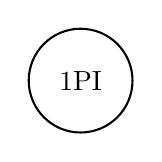
\begin{tikzpicture}[x=0.75pt,y=0.75pt,yscale=-1,xscale=1]
                %uncomment if require: \path (0,300); %set diagram left start at 0, and has height of 300
                
                %Shape: Circle [id:dp8588117224452179] 
                \draw   (100,144) .. controls (100,130.19) and (111.19,119) .. (125,119) .. controls (138.81,119) and (150,130.19) .. (150,144) .. controls (150,157.81) and (138.81,169) .. (125,169) .. controls (111.19,169) and (100,157.81) .. (100,144) -- cycle ;
                
                % Text Node
                \draw (125,144) node   [align=left] {1PI};
                \end{tikzpicture}
        \end{gathered},
    \]
    或者说
    \begin{equation}
        \frac{1}{G} = \frac{1}{G^0} - \Sigma, \quad 
        -\Sigma = \begin{gathered}
            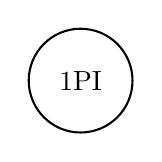
\begin{tikzpicture}[x=0.75pt,y=0.75pt,yscale=-1,xscale=1]
                %uncomment if require: \path (0,300); %set diagram left start at 0, and has height of 300
                
                %Shape: Circle [id:dp8588117224452179] 
                \draw   (100,144) .. controls (100,130.19) and (111.19,119) .. (125,119) .. controls (138.81,119) and (150,130.19) .. (150,144) .. controls (150,157.81) and (138.81,169) .. (125,169) .. controls (111.19,169) and (100,157.81) .. (100,144) -- cycle ;
                
                % Text Node
                \draw (125,144) node   [align=left] {1PI};
                \end{tikzpicture}
        \end{gathered},
    \end{equation}
    即单电子(或者别的什么粒子)带相互作用的格林函数的极点展示的能量相比自由格林函数要减去1PI图或者说加上$\Sigma$,这就是所谓自能修正。

    对零温场论同样有自能修正,为
    \begin{equation}
        \frac{1}{\ii G} = \frac{1}{\ii G^0} + \ii \Sigma, \quad - \ii \Sigma = \begin{gathered}
            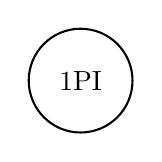
\begin{tikzpicture}[x=0.75pt,y=0.75pt,yscale=-1,xscale=1]
                %uncomment if require: \path (0,300); %set diagram left start at 0, and has height of 300
                
                %Shape: Circle [id:dp8588117224452179] 
                \draw   (100,144) .. controls (100,130.19) and (111.19,119) .. (125,119) .. controls (138.81,119) and (150,130.19) .. (150,144) .. controls (150,157.81) and (138.81,169) .. (125,169) .. controls (111.19,169) and (100,157.81) .. (100,144) -- cycle ;
                
                % Text Node
                \draw (125,144) node   [align=left] {1PI};
                \end{tikzpicture}
        \end{gathered}.
    \end{equation}

    1PI图的计算常常采用骨架图的做法,即画出1PI图中最低阶的那些图,然后将其中的粒子线和相互作用顶角替换成相互作用修饰后的,这样可以覆盖全部1PI图。
\end{back}

\begin{back}{平均场近似}{scf-method}
    一种常用的近似是,在1PI图中只将我们想要计算的那部分单粒子格林函数对应的粒子线替换成相互作用粒子线,于是得到一个形如“我们想要计算的单粒子格林函数=一系列包含我们想要计算的单粒子格林函数的费曼图的和”这样的方法,即可解出我们想要计算的单粒子格林函数。
    形式上,这等价于将相互作用哈密顿量做类似于这样的分解:
    \[
        c^\dagger c^\dagger c c \approx \expval{c^\dagger c} c^\dagger c,
    \]
    其中$\expval{c^\dagger c}$是我们要计算的格林函数,然后用这个“单电子哈密顿量”形式地求解$\expval{c^\dagger c}$,就得到了一个自洽方程,解之就得到想要的格林函数。
    形式上看,这相当于将相互作用看成了系统中其它粒子形成的大小为$\expval{c^\dagger c}$的一个外场,所以也可以叫做平均场近似。

    以上介绍的是需要求解自洽方程的平均场近似,当然作为最粗糙的估计,这个自洽方程的右边可以代入自由情况下我们要计算的格林函数,这就是非自洽的平均场方法,通常效果不好。
\end{back}

计算单电子格林函数实际上就是要计算自能。本节考虑库伦相互作用的平均场理论,即将一阶自能图中的所有电子线修正为相互作用电子线,不对相互作用线和顶角做修正。
这样会得到

\subsubsection{零温下的HF自洽方程组}

\subsubsection{有限温度情况}

\subsubsection{Hartree-Fock近似的用处以及它何时失效}

\begin{figure}
    \centering
    

\tikzset{every picture/.style={line width=0.75pt}} %set default line width to 0.75pt        

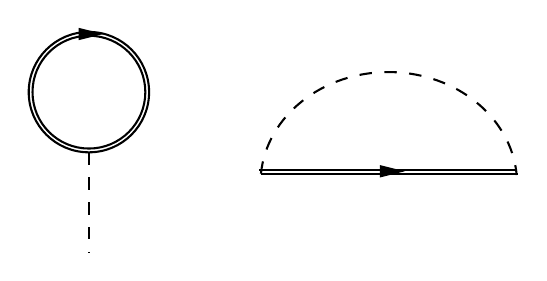
\begin{tikzpicture}[x=0.75pt,y=0.75pt,yscale=-1,xscale=1]
%uncomment if require: \path (0,300); %set diagram left start at 0, and has height of 300

%Shape: Circle [id:dp7062631080857045] 
\draw   (122.85,160.48) .. controls (122.85,144.46) and (135.84,131.48) .. (151.85,131.48) .. controls (167.87,131.48) and (180.85,144.46) .. (180.85,160.48) .. controls (180.85,176.5) and (167.87,189.48) .. (151.85,189.48) .. controls (135.84,189.48) and (122.85,176.5) .. (122.85,160.48) -- cycle ;
%Straight Lines [id:da045289897075393215] 
\draw    (158.85,132.48) ;
\draw [shift={(158.85,132.48)}, rotate = 180] [fill={rgb, 255:red, 0; green, 0; blue, 0 }  ][line width=0.08]  [draw opacity=0] (12,-3) -- (0,0) -- (12,3) -- cycle    ;
%Shape: Circle [id:dp5875221682694243] 
\draw   (124.68,160.48) .. controls (124.68,145.47) and (136.84,133.3) .. (151.85,133.3) .. controls (166.86,133.3) and (179.03,145.47) .. (179.03,160.48) .. controls (179.03,175.49) and (166.86,187.66) .. (151.85,187.66) .. controls (136.84,187.66) and (124.68,175.49) .. (124.68,160.48) -- cycle ;
%Straight Lines [id:da33094867749017665] 
\draw    (234,198) -- (357.71,198) ;
%Shape: Arc [id:dp010998921926927085] 
\draw  [draw opacity=0][dash pattern={on 4.5pt off 4.5pt}] (234.74,199.78) .. controls (237.47,172.1) and (264.31,150.53) .. (296.82,150.82) .. controls (329.13,151.12) and (355.45,172.9) .. (357.95,200.4) -- (296.33,204.56) -- cycle ; \draw  [dash pattern={on 4.5pt off 4.5pt}] (234.74,199.78) .. controls (237.47,172.1) and (264.31,150.53) .. (296.82,150.82) .. controls (329.13,151.12) and (355.45,172.9) .. (357.95,200.4) ;
%Straight Lines [id:da4279592316148173] 
\draw    (304,198.62) ;
\draw [shift={(304,198.62)}, rotate = 180] [fill={rgb, 255:red, 0; green, 0; blue, 0 }  ][line width=0.08]  [draw opacity=0] (12,-3) -- (0,0) -- (12,3) -- cycle    ;
%Straight Lines [id:da7235406851190553] 
\draw  [dash pattern={on 4.5pt off 4.5pt}]  (151.85,189.48) -- (151.85,237.5) ;
%Straight Lines [id:da6319302703930361] 
\draw    (234.74,199.78) -- (358.44,199.78) ;




\end{tikzpicture}

    \caption{一般的电子-电子散射也有Hartree项和Fock项}
    \label{fig:generalized-hartree-fock}
\end{figure}

以上推导都是针对库仑相互作用的,但是显然对\eqref{eq:general-electron-electron-interaction}中一般的电子-电子相互作用,由于存在动量转移,从高能物理的角度说,由于有光子交换,电子-电子相互作用顶角仍然需要包含相互作用线(此时绘制为虚线,因为没有特别良定义的“光子”概念),为
\begin{equation}
    \begin{gathered}
        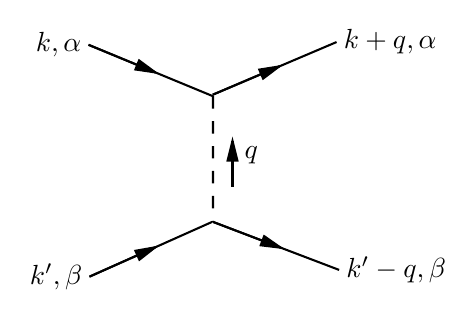
\begin{tikzpicture}[x=0.75pt,y=0.75pt,yscale=-1,xscale=1]
            %uncomment if require: \path (0,300); %set diagram left start at 0, and has height of 300
            %Straight Lines [id:da6810974252980533] 
            \draw    (120.17,187.49) -- (151.95,173.3) ;
            \draw [shift={(153.77,172.48)}, rotate = 515.9300000000001] [fill={rgb, 255:red, 0; green, 0; blue, 0 }  ][line width=0.08]  [draw opacity=0] (12,-3) -- (0,0) -- (12,3) -- cycle    ;
            %Straight Lines [id:da40733827497945274] 
            \draw    (120.17,187.49) -- (179.26,161.1) ;
            
            %Straight Lines [id:da4271611228799128] 
            \draw    (179.7,161.1) -- (212.38,173.55) ;
            \draw [shift={(214.25,174.26)}, rotate = 200.85] [fill={rgb, 255:red, 0; green, 0; blue, 0 }  ][line width=0.08]  [draw opacity=0] (12,-3) -- (0,0) -- (12,3) -- cycle    ;
            %Straight Lines [id:da753337349268864] 
            \draw    (179.7,161.1) -- (240.46,184.24) ;
            
            %Straight Lines [id:da09481485705124859] 
            \draw    (119.72,75.78) -- (151.97,89.1) ;
            \draw [shift={(153.82,89.87)}, rotate = 202.44] [fill={rgb, 255:red, 0; green, 0; blue, 0 }  ][line width=0.08]  [draw opacity=0] (12,-3) -- (0,0) -- (12,3) -- cycle    ;
            %Straight Lines [id:da7578837470001811] 
            \draw    (119.72,75.78) -- (179.69,100.55) ;
            
            %Straight Lines [id:da7058048331027083] 
            \draw    (179.57,99.82) -- (211.65,86.18) ;
            \draw [shift={(213.49,85.39)}, rotate = 516.96] [fill={rgb, 255:red, 0; green, 0; blue, 0 }  ][line width=0.08]  [draw opacity=0] (12,-3) -- (0,0) -- (12,3) -- cycle    ;
            %Straight Lines [id:da4335041927311629] 
            \draw    (179.57,99.82) -- (239.22,74.45) ;
            
            %Straight Lines [id:da2943384130706994] 
            \draw    (189.09,144.08) -- (189.09,122.03) ;
            \draw [shift={(189.09,120.03)}, rotate = 450] [fill={rgb, 255:red, 0; green, 0; blue, 0 }  ][line width=0.08]  [draw opacity=0] (12,-3) -- (0,0) -- (12,3) -- cycle    ;
            %Straight Lines [id:da5722731848454237] 
            \draw  [dash pattern={on 4.5pt off 4.5pt}]  (179.69,100.55) -- (179.7,161.1) ;
            
            % Text Node
            \draw (117.72,75.78) node [anchor=east] [inner sep=0.75pt]    {$\boldsymbol{k} ,\alpha $};
            % Text Node
            \draw (241.22,74.45) node [anchor=west] [inner sep=0.75pt]    {$\boldsymbol{k} +\boldsymbol{q} ,\alpha $};
            % Text Node
            \draw (193.48,123.48) node [anchor=north west][inner sep=0.75pt]    {$\boldsymbol{q}$};
            % Text Node
            \draw (118.17,187.49) node [anchor=east] [inner sep=0.75pt]    {$\boldsymbol{k} ',\beta $};
            % Text Node
            \draw (242.46,184.24) node [anchor=west] [inner sep=0.75pt]    {$\boldsymbol{k} '-\boldsymbol{q} ,\beta $};
            \end{tikzpicture}
    \end{gathered} = - \frac{1}{\beta} \sum_{\omega_n} \int \frac{\dd[3]{\vb*{q}}}{(2\pi)^3} V_{\vb*{q}}  ,
\end{equation}
因此\eqref{eq:general-electron-electron-interaction}关于单电子格林函数的平均场近似同样包含Hartree项和Fock项(见\autoref{fig:generalized-hartree-fock}),同样可以称为Hartree-Fock近似。

Hartree-Fock近似成立的条件是相互作用线修正和顶角修正可以略去,在这些说法不适用的情况下,自然就不正确了。

\subsection{RPA近似}

实际上从\eqref{eq:ext-electron-ret-nn}就可以看出RPA近似的实质。将\eqref{eq:ext-electron-ret-nn}做级数展开,我们有
\[
    G^\text{ret}_{nn}(\vb*{k}, \omega) = G^\text{0, ret}_{nn}(\vb*{k}, \omega) + G^\text{0, ret}_{nn}(\vb*{k}, \omega) \frac{4\pi e^2}{k^2} G^\text{0, ret}_{nn}(\vb*{k}, \omega) + \cdots,
\]
上式两边加上电子数密度平方,并注意到$G^\text{0, ret}_{nn}(\vb*{k}, \omega)$就是电子-空穴组成的环的贡献——依照定义,自由电子的密度-密度格林函数为
\[
    \begin{aligned}
        G_{nn}^\text{0}(\vb*{r}-\vb*{r}', \tau-\tau') &= - T_\tau \expval*{\var{{n}}(\vb*{r}, \tau) \var{{n}}(\vb*{r}', \tau')} \\
        &= - T_\tau \expval*{{{n}}(\vb*{r}, \tau) {{n}}(\vb*{r}', \tau')} + \expval*{{n}(\vb*{r}, \tau)} \expval*{{n}(\vb*{r}', \tau')} \\
        &= \sum_{\sigma, \sigma'} T_\tau \expval*{{\psi}_{\sigma'}(\vb*{r}', \tau') {\psi}^\dagger_\sigma(\vb*{r}, \tau)} T_\tau \expval*{ {\psi}_\sigma(\vb*{r}, \tau) {\psi}^\dagger_{\sigma'}(\vb*{r}', \tau') } ,
    \end{aligned}
\]
其中最后一个等号用到了Wick定理——我们就发现\eqref{eq:ext-electron-ret-nn}实际上就是环形图近似。
\eqref{eq:ext-electron-ret-nn}实际上给出了$G^\text{ret}_{nn}$中最为奇异的部分,因为环形图会产生次数非常高的$1/k^n$型的项,从而发散得最厉害;但是将所有这些发散的图求和起来却能够得到一个收敛的结果。
环形图近似的成立条件是粒子数密度很高,从而主要的相互作用形式是电子通过库仑相互作用,激发出一些电子-空穴对(即环形图中的环),即主要的相互作用是环形图。
也可以从另一个角度理解这件事:粒子数密度较高意味着屏蔽作用很强,所以$1/k^n$发散得不那么厉害的那些项没有什么贡献。
RPA近似下没有出现这样的图:一个电子回线内部有一条光子线,即在单电子回线的图中没有出现Fock项,这和托马斯-费米屏蔽的假设是一致的,因此确实可以预期,当$\omega \to 0$时RPA近似退化到托马斯-费米屏蔽上。

\subsection{梯形图近似}

\section{金属和朗道费米液体}\label{sec:landau-fermi-liquid}

\concept{朗道费米液体}是一个这样的低能有效理论,其基本假设为:
\begin{enumerate}
    \item 费米液体的状态可以和费米气体一样,使用某种费米型自旋$1/2$准粒子的占据数标记,并且系统能量可以写成占据数的函数。
    这个假设对哈密顿量的形式做出了很强的限制,因为此时的哈密顿量已经在粒子数表象下被严格对角化了。(但是这个哈密顿量仍然可以不是自由哈密顿量,因为可以有密度-密度相互作用)不过我们将会看到,这样的限制是合理的。
    \item 当相互作用趋于零(“被关闭”)时,费米液体态回退到实际的费米气体态,我们假设此时费米液体态的占据数和实际的费米气体态的占据数相同。
    这个假设实际上是说,费米液体中的占据数所描述的准粒子实际上是经过某种重整化的电子,和电子可以一一对应。
\end{enumerate}

可以从费米液体中准粒子的行为中看到很明显的普通电子的影子:准粒子场和电子场的对称性相同,准粒子也是费米子,准粒子能谱和电子能谱形式类似,自旋均为$1/2$,带电量相同,等等。
唯象的讨论中可以直接将费米液体中的准粒子当成电子。

到这里我们其实并不知道费米液体中的准粒子到底是什么。
可以通过这样的方式想象费米液体可以怎样产生:对无相互作用的能带电子%
\footnote{
    应当注意能带电子这个名称本身有些模糊不清。只计算周期性势场的影响可以得到能带,只计算经过平滑处理的赝势也可以得到能带,将一部分相互作用作为自能修正而留下最为显著的相互作用通道作为碰撞也可以得到能带(虽然还需要额外计算碰撞的影响,如费米液体中那样),对很多系统,其实相互作用全都考虑进去了还是可以得到能带——如同用DFT计算出来的那样。
    例如,在费米液体中,如果粒子数涨落不大,完全可以用粒子数平均值代替相互作用项中的准粒子占据数。
    即使相互作用大一些,也可以理解成“能带被拉歪了”。
}%
,我们可以绝热地将相互作用加入,如果没有出现诸如费米子配对之类让系统能谱结构发生很大变化的情况,那么第二个假设就已经满足了。
相互作用会导致电子出现自能修正,由于库仑相互作用的顶角是保持粒子数守恒的,不存在一个电子衰变成多个其它粒子的过程,因此自能修正是实数,即单电子态的确是本征态。%
\footnote{
    虽然如此,如果我们将高于费米面的电子称为电子而将低于费米面的电子称为空穴,那么的确可以出现一个电子和费米球中的空穴发生相互作用,而衰变成电子和空穴的过程。
    见\autoref{sec:fermi-liquid-ground}。
}%
在很多粒子数守恒的理论——如$\phi^4$理论或是QED——中,可以有稳定的单粒子、二粒子、三粒子……本征态,虽然$n$粒子态的能量不是$n$个粒子的能量简单相加,但是无论如何,一个本征态的能量可以写成各个动量上的粒子的占据数的函数,因此量子态可以用占据数标记,能量也可以用粒子数标记,即第一个假设也是成立的。

对那些确定是从相互作用电子系统产生出来的费米液体,准粒子的动量就是电子的动量。
这是因为,在关闭相互作用时费米液体“无缝地”退化到实际的费米气体上,因此在无相互作用点处费米液体中准粒子的动量就是实际的能带电子的动量。
现在缓慢地加上相互作用,则费米液体准粒子的动量可以发生连续变化,但有限体系中动量实际上是分立的,从而动量只能不变。
因此,准粒子的动量实际上就是电子的动量。
然而动量守恒和粒子数没有关系,设$\ket{\Psi}$是费米液体的基态而$c^\dagger_{\vb*{k}}$是Bloch电子的产生算符,则$c^\dagger_{\vb*{k}} \ket{\Psi}$\emph{不是}$n_{\vb*{k}}$精确地加一的态,而是多出来一个电子位于$\vb*{k}$上、多出来两个电子位于$\vb*{k}$上和一个空穴位于$-\vb*{k}$上、多出来三个电子位于$\vb*{k}$上和两个空穴位于$-\vb*{k}$上这一系列态的叠加。
费米液体中的准粒子是能带电子重整化得到的,这个过程可以线性组合$c_{\vb*{k}}$和$c^\dagger_{\vb*{k}}$。
这也意味着无法保证费米液体的准粒子的费米面和产生费米液体的含有库伦散射的多电子系统在不考虑库伦散射时的费米面高度是一样的。

在什么情况下费米液体理论失效?如果相互作用是吸引的,那么低温下可能出现费米子配对,此时总是会出现相变。
还有一些情况下相互作用会导致电子在空间上排列成一定的模式,此时也会出现相变,因为出现了新的序。
我们将在\autoref{chap:low-and-super}中讨论这些情况。
如果相互作用较强,能带的图像甚至可能就完全不适用了,此时系统的元激发可能都不是经过修正的电子,也无所谓费米液体。
令人震惊的是,虽然大部分实际体系中库仑相互作用的确很强,并且显然不只有密度-密度相互作用通道,费米液体图像仍然是适用的。

\subsection{基态附近的激发}\label{sec:fermi-liquid-ground}

与高能物理中不同,实际的凝聚态体系的基态中都有\emph{大量}准粒子。由于准粒子是费米子,系统基态中有一个费米球。
由于粒子数守恒,系统基态附近的激发态就是一些准粒子从费米球内部被打到费米球外部之后形成的,并且距离费米面均不远。
因此其实我们可以忽略费米海而认为系统中实际上有两种元激发:“电子”和“空穴”,而所谓的费米面就是区分电子和空穴的一个边界。

在费米液体理论中通常也只分析费米面附近的物理,部分原因在于费米海的结构可以非常复杂,因此只考虑费米面附近的物理是比较容易的,也是比较有实际意义的(因为是低温近似),部分原因在于只有这里才确定有稳定的准粒子——通常准粒子的寿命在接近费米面时比较长,因此看起来像是“真正的”粒子(否则会有非常明显的能级展宽)。

\begin{figure}
    \centering
    

    \tikzset{every picture/.style={line width=0.75pt}} %set default line width to 0.75pt        

    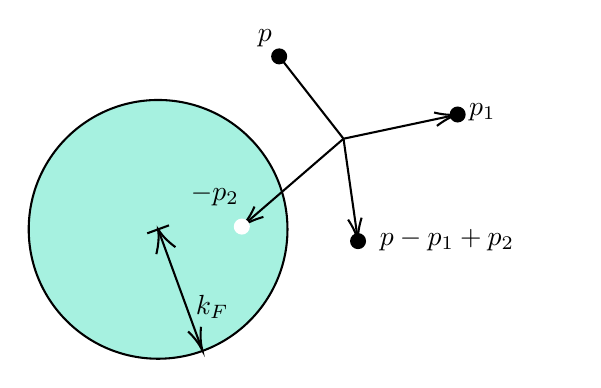
\begin{tikzpicture}[x=0.75pt,y=0.75pt,yscale=-1,xscale=1]
    %uncomment if require: \path (0,300); %set diagram left start at 0, and has height of 300

    %Shape: Circle [id:dp4115009856655256] 
    \draw  [fill={rgb, 255:red, 80; green, 227; blue, 194 }  ,fill opacity=0.51 ] (166.33,128.33) .. controls (166.33,93.91) and (194.24,66) .. (228.67,66) .. controls (263.09,66) and (291,93.91) .. (291,128.33) .. controls (291,162.76) and (263.09,190.67) .. (228.67,190.67) .. controls (194.24,190.67) and (166.33,162.76) .. (166.33,128.33) -- cycle ;
    %Straight Lines [id:da36238650054186783] 
    \draw    (428,157) ;
    %Straight Lines [id:da7864189605567815] 
    \draw    (228.67,128.33) -- (249.31,184.79) ;
    \draw [shift={(250,186.67)}, rotate = 249.91] [color={rgb, 255:red, 0; green, 0; blue, 0 }  ][line width=0.75]    (10.93,-3.29) .. controls (6.95,-1.4) and (3.31,-0.3) .. (0,0) .. controls (3.31,0.3) and (6.95,1.4) .. (10.93,3.29)   ;
    \draw [shift={(228.67,128.33)}, rotate = 69.91] [color={rgb, 255:red, 0; green, 0; blue, 0 }  ][line width=0.75]    (0,5.59) -- (0,-5.59)(10.93,-4.9) .. controls (6.95,-2.3) and (3.31,-0.67) .. (0,0) .. controls (3.31,0.67) and (6.95,2.3) .. (10.93,4.9)   ;
    %Straight Lines [id:da9264496937896287] 
    \draw    (287,45) ;
    \draw [shift={(287,45)}, rotate = 0] [color={rgb, 255:red, 0; green, 0; blue, 0 }  ][fill={rgb, 255:red, 0; green, 0; blue, 0 }  ][line width=0.75]      (0, 0) circle [x radius= 3.35, y radius= 3.35]   ;
    %Straight Lines [id:da7148452328407287] 
    \draw    (325,134) ;
    \draw [shift={(325,134)}, rotate = 0] [color={rgb, 255:red, 0; green, 0; blue, 0 }  ][fill={rgb, 255:red, 0; green, 0; blue, 0 }  ][line width=0.75]      (0, 0) circle [x radius= 3.35, y radius= 3.35]   ;
    %Straight Lines [id:da9678432617223967] 
    \draw    (373,73) ;
    \draw [shift={(373,73)}, rotate = 0] [color={rgb, 255:red, 0; green, 0; blue, 0 }  ][fill={rgb, 255:red, 0; green, 0; blue, 0 }  ][line width=0.75]      (0, 0) circle [x radius= 3.35, y radius= 3.35]   ;
    %Straight Lines [id:da9966061673025197] 
    \draw    (287,45) -- (318,84.67) ;
    %Straight Lines [id:da6540000533421391] 
    \draw    (318,84.67) -- (270.51,125.69) ;
    \draw [shift={(269,127)}, rotate = 319.16999999999996] [color={rgb, 255:red, 0; green, 0; blue, 0 }  ][line width=0.75]    (10.93,-3.29) .. controls (6.95,-1.4) and (3.31,-0.3) .. (0,0) .. controls (3.31,0.3) and (6.95,1.4) .. (10.93,3.29)   ;
    %Straight Lines [id:da2459804058265671] 
    \draw [color={rgb, 255:red, 255; green, 255; blue, 255 }  ,draw opacity=1 ][fill={rgb, 255:red, 255; green, 255; blue, 255 }  ,fill opacity=1 ]   (269,127) ;
    \draw [shift={(269,127)}, rotate = 0] [color={rgb, 255:red, 255; green, 255; blue, 255 }  ,draw opacity=1 ][fill={rgb, 255:red, 255; green, 255; blue, 255 }  ,fill opacity=1 ][line width=0.75]      (0, 0) circle [x radius= 3.35, y radius= 3.35]   ;
    %Straight Lines [id:da8849358294167189] 
    \draw    (318,84.67) -- (324.72,132.02) ;
    \draw [shift={(325,134)}, rotate = 261.92] [color={rgb, 255:red, 0; green, 0; blue, 0 }  ][line width=0.75]    (10.93,-3.29) .. controls (6.95,-1.4) and (3.31,-0.3) .. (0,0) .. controls (3.31,0.3) and (6.95,1.4) .. (10.93,3.29)   ;
    %Straight Lines [id:da5006771127819694] 
    \draw    (318,84.67) -- (371.04,73.42) ;
    \draw [shift={(373,73)}, rotate = 528.02] [color={rgb, 255:red, 0; green, 0; blue, 0 }  ][line width=0.75]    (10.93,-3.29) .. controls (6.95,-1.4) and (3.31,-0.3) .. (0,0) .. controls (3.31,0.3) and (6.95,1.4) .. (10.93,3.29)   ;

    % Text Node
    \draw (245.33,158.5) node [anchor=north west][inner sep=0.75pt]    {$k_{\text{F}}$};
    % Text Node
    \draw (285,42) node [anchor=south east] [inner sep=0.75pt]    {$\boldsymbol{p}$};
    % Text Node
    \draw (377,72) node [anchor=west] [inner sep=0.75pt]    {$\boldsymbol{p}_{1}$};
    % Text Node
    \draw (243,105) node [anchor=north west][inner sep=0.75pt]    {$-\boldsymbol{p}_{2}$};
    % Text Node
    \draw (334,127) node [anchor=north west][inner sep=0.75pt]    {$\boldsymbol{p} -\boldsymbol{p}_{1} +\boldsymbol{p}_{2}$};


    \end{tikzpicture}


    \caption{一个准粒子衰变成两个准粒子和一个准空穴,或者说准粒子费米海中的一个准粒子被激发到费米面以上}
    \label{fig:quasi-particle-damping-example}
\end{figure}

这件事的原因如下。首先应当注意,虽然准粒子的自能修正总是实数,从而,在没有其它任何准粒子时,单个准粒子可以永远稳定存在而不会衰变,但与高能物理中的情况不同,费米球的存在意味着如果费米面上方出现了一个准粒子,它会激发费米海内部的准粒子,从而产生一个空穴,正如\autoref{fig:quasi-particle-damping-example}所示。
因此,在基态(不是真空态,而是带有费米球的态),费米面上方的准粒子的确会发生衰变。
将费米面上方的准粒子和费米球内部的空穴看成两种元激发可以更加清楚地看到这一点:此时费米面上方的准粒子的个数根本不是守恒的(从而,积掉费米海会产生一个非幺正的理论),从而其自能修正不可能是实数。
这是含有相互作用的多粒子态的一般特征:在这种态中没有非常“尖锐”的单粒子极点。

设准粒子寿命为$\tau$,则$\tau$反比于散射速率,而散射速率正比于库仑散射的强度。完整地做这个计算是很困难的,因为涉及到静电屏蔽等复杂的效应。
散射的过程可以概括为:一个动量为$\vb*{p}$的费米面外部的准粒子的能量降低,变成了动量为$\vb*{p}_1$的准粒子,同时激发了一个费米面内的动量为$\vb*{p}_2$的准粒子。
结果是,动量为$\vb*{p}$的费米面以外的准粒子衰变成了两个准粒子,动量分别为$\vb*{p}_1$和$\vb*{p} - \vb*{p}_1 + \vb*{p}_2$,还有一个动量为$-\vb*{p}_2$的空穴。
如果这种散射实际上很少发生,那么就能够有稳定的准粒子。

设我们通过若干轮重整化群计算,已经得到了一种有费米型自旋$1/2$的准粒子,且符合费米液体的第二个假设的有效理论。
假设准粒子之间的相互作用强度不非常强地依赖于动量,不妨记作$M$(纯粹的库伦相互作用\emph{不满足}这个条件,它强烈依赖入射电子的动量差,因此即使在费米面附近,相互作用强度也不能当作常数,因此能带电子加入库伦相互作用后并不严格就是稳定的准粒子,而仍然需要经过几轮重整化,让$M$变得“柔和”一些)。
我们至此还没有确定这个系统是费米液体,因为其中准粒子之间有散射,不同动量上的准粒子数目有涨落。
在这样的系统中,动量分别为$\vb*{p}_1$和$\vb*{p} - \vb*{p}_1 + \vb*{p}_2$的两个准粒子和动量为$\vb*{p}_2$的空穴的联合态密度在当前温度下的期望值为$n$,由费米黄金法则有
\[
    \frac{1}{\tau} \propto \text{transition rate} \sim \abs{M}^2 n.
\]
由于系统中的准粒子非常多,不同能级上准粒子数的涨落可以略去,即认为不同能级上不多不少正好就有费米-狄拉克分布给出的粒子个数,%
\footnote{这是热力学系统的一般性质:系统规模大时涨落可略去。由于本文涉及的系统都是多体系统,总是可以做这样的近似。}%
那么就有
\[
    n = \int \dd[3]{\vb*{p}_1} \int \dd[3]{\vb*{p}_2} (1 - f(\epsilon_{\vb*{p}_1})) f(\epsilon_{\vb*{p}_2}) (1 - f(\epsilon_{\vb*{p} - \vb*{p}_1 + \vb*{p}_2})) \delta(\epsilon_{\vb*{p}} - \epsilon_{\vb*{p}_1} + \epsilon_{\vb*{p}_2} - \epsilon_{\vb*{p} - \vb*{p}_1 + \vb*{p}_2}).
\]
因子$(1-\epsilon_{\vb*{p}_1})$表示动量为$\vb*{p}_1$的粒子应该占据一个空态(或者说在接近零温时应该在费米面以外),因子$f(\epsilon_{\vb*{p}_2})$表示空穴一定来自一个已有的粒子,最后的$\delta$函数强制要求能量守恒。
我们不严格计算这个积分,而是做一些数量级估计。
由于$\vb*{p}_2$在费米面以下而$\vb*{p}- \vb*{p}_1 + \vb*{p}_2$在费米面以上,容易写出以下不等式
\[
    0 < \xi_{\vb*{p}_1} < \xi_{\vb*{p}}, \quad 0 < - \xi_{\vb*{p}_2} < \xi_{\vb*{p}} - \xi_{\vb*{p}_1} < \xi_{\vb*{p}},
\]
对$n$有贡献的$\vb*{p}_1$和$\vb*{p}_2$均满足这些不等式,这些不等式给出了两个宽度为$\xi_{\vb*{p}}$的球壳,因此
\[
    n \leq (4 \pi k_\text{F}^2 \xi_{\vb*{p}})^2,
\]
于是
\begin{equation}
    \frac{1}{\tau} \lesssim \xi_{\vb*{p}}^2.
\end{equation}
因此,如果准粒子非常接近费米液体的费米面,那么它是非常稳定的,因为此时$\xi_{\vb*{p}}$很小。从物理图像上看,此时的准粒子虽然会和费米海中的准粒子发生相互作用,但其能量不足以产生粒子-空穴对,因此也不会衰变。

总之,准粒子之间的碰撞不可忽略意味着费米面以上的准粒子会衰变。
然而,在费米面附近,这种衰变是非常缓慢的,以至于我们可以认为任何一种动量确定的准粒子分布都可以长期稳定存在,即哈密顿量在以动量标记的粒子数表象下是对角化的,从而费米液体理论的第一个假设成立。

从上面的论述可以看出,对相当大的一类相互作用电子气系统,\emph{只有}在费米面附近第一个假设才是严格成立的,在稍微远离费米面的地方,准粒子之间仍然有碰撞。
显然,准粒子完全没有碰撞的情况只适用于这种电子气系统的红外极限。
几乎所有凝聚态系统都处在接近热平衡的状态,温度提供了一个好的能标,因此费米液体理论的适用条件就转化成了这样一个问题:热涨落是不是足够让准粒子之间的碰撞体现出来?
换句话说,动量确定的准粒子寿命是否长到\emph{热涨落}的时间尺度?
或者等价地说,由于碰撞导致的准粒子能级展宽相比于费米-狄拉克分布函数关于能量的变化尺度是不是可以忽略的?

我们首先估算电子平均自由时间。按照费米-狄拉克分布,$\expval*{{n}}$在$\epsilon_\text{F}$附近一个大约长为$T$的区域内明显偏离阶跃函数;只有这个“弥散区域”内的电子会发生散射(费米球内部的准粒子不怎么会被激发,费米球外面根本没有准粒子)。
发生一次散射需要两个来自弥散区域的电子,因此
\[
    \frac{1}{\tau} \sim T^2,
\]
即
\begin{equation}
    \tau \sim \frac{1}{T^2},
\end{equation}
准粒子平均自由时间本身和温度有关。
另一方面,碰撞导致能量本身出现弥散,为%
\footnote{
    注意不确定性关系在混合态中也是有的。
}%
\[
    \Delta E \sim \frac{1}{\Delta t} \sim \frac{1}{\tau},
\]
其中$\tau$为准粒子平均自由时间。如前所述,有稳定准粒子等价于
\[
    \Delta E \ll \frac{1}{T},
\]
也即
\[
    \frac{1}{\tau} \ll T.
\]
最后就发现我们有
\begin{equation}
    T \ll 1.
\end{equation}
因此费米液体图像只在低温下适用。

\subsection{哈密顿量和前向散射相互作用}

费米液体的能级结构和费米气体完全一致并不意味着库伦相互作用完全不产生任何影响,因为每个能级具体的能量大小可以经历修正。
这意味着准粒子的哈密顿量并不是简单的
\[
    H = \sum_{\vb*{k}, \sigma} \epsilon_{\vb*{k}} n_{\vb*{k} \sigma},
\]
而有一些高阶项,它们表示密度-密度相互作用。

考虑一个能量本征态,其中准粒子在费米面之上的数量为$\var{n}$($\delta$表示相对基态的偏离,正表示有粒子,负表示有空穴)。
考虑到费米液体理论的第一条假设,把能量本征值相对于零温平衡态(由于费米海的结构可以非常复杂,零温能量反而是算不出来的,我们也不需要计算它)的变化写成以下级数展开($\vb*{k}$在费米面附近):
\begin{equation}
    \var{E} = \underbrace{\sum_{\vb*{k}, \sigma} \epsilon^0_{\vb*{k}} \var{n_{\vb*{k} \sigma}}}_{\var{E_1}} + \underbrace{\frac{1}{2V} \sum_{\vb*{k}, \vb*{k}', \sigma, \sigma'} f_{\sigma \sigma' \vb*{k} \vb*{k}'} \var{n_{\vb*{k} \sigma}} \var{n_{\vb*{k}' \sigma'}}}_{\var{E_2}},
    \label{eq:fermi-liquid-energy}
\end{equation}
其中$\var{n}$表示准粒子数目相对基态的变化。把能量写成粒子数的函数假定了自旋守恒。对动量做求和化积分,就得到
\begin{equation}
    \frac{\var{E}}{V} = \underbrace{\sum_{\sigma} \int \frac{\dd[3]{\vb*{k}}}{(2\pi)^3} \epsilon^0_{\vb*{k}} \var{n_{\vb*{k} \sigma}}}_{\var{E_1} / V} + \underbrace{\frac{1}{2} \sum_{\sigma, \sigma'} \int \frac{\dd[3]{\vb*{k}}}{(2\pi)^3} \int \frac{\dd[3]{\vb*{k}'}}{(2\pi)^3} f_{\sigma \sigma' \vb*{k} \vb*{k}'} \var{n_{\vb*{k} \sigma}} \var{n_{\vb*{k}' \sigma'}}}_{\var{E_2} / V}
\end{equation}
我们保留到二阶项,一阶项给出准粒子的近独立理论,二阶项给出准粒子的相互作用。
这种相互作用并不会让粒子数发生涨落或是让单个准粒子的动量发生涨落,而只会对能级做修正,是所谓的“前向散射”。
会让准粒子动量发生变化的那部分相互作用或者说“碰撞”,正如上一节所说,需要略微远离一些费米面才看得到,没有体现在\eqref{eq:fermi-liquid-energy}中。

重整化群可能给出更高阶项,而也许二阶项实际上可以忽略,而绕了一大圈之后发现$\abs{M}$很小,从而实际上在很大的区域内费米液体图像均适用。
为了表明我们保留到二阶项是正确的,我们给出一个数量级估计,说明一阶项和二阶项的量级是同阶的,而低于更高阶项。
我们知道由于相互作用的存在,总能量$E$肯定不是单粒子哈密顿量(比如说$k^2/2m$这种形式)的期望值简单加起来的结果,但是显然能量具有可加性,设想我们改变了准粒子数分布,这样应该有
\[
    \var{E} = \sum_{\vb*{k}, \sigma} \epsilon_{\vb*{k} \sigma} \var{n_{\vb*{k} \sigma}},
\]
其中$\epsilon_{\vb*{k}}$是在有限温度下的近平衡态激发一个准粒子的能量,它的一部分是单准粒子能量,一部分是其它准粒子给它的相互作用能之和。
因此,$\epsilon_{\vb*{k}}$会依赖准粒子数分布。由于我们只研究二体相互作用,我们有
\[
    \epsilon \sim \sum_{\vb*{k}'} \text{something} \cdot n_{\vb*{k}'},
\]
于是设
\[
    \var{\epsilon_{\vb*{k} \sigma}} = \frac{1}{V} \sum_{\vb*{k}', \sigma'} f_{\sigma \sigma' \vb*{k} \vb*{k}'} \var{n_{\vb*{k}' \sigma'}},
\]
记$\epsilon_{\vb*{k}}^0$为$n_{\vb*{k}}$一概为零的$\epsilon_{\vb*{k}}$,代入$\var{E}$中就得到\eqref{eq:fermi-liquid-energy};第二项的$1/2$因子是因为一对粒子会被计数两次,所以要除以$2$;由于我们假定准粒子分布相对于零温只有微小的偏离,$\epsilon_{\vb*{k}}$被取为零温的值。
虽然$\epsilon^0 \var{n}$看起来比$f\var{n} \var{n}$大,但需要注意到我们在巨正则系综中工作,则真的有意义的应该是$E-\mu N$(且由于是近平衡,应有$\var{E} = \mu \var{N}$),而
\[
    \sum_{\vb*{k}} (\epsilon^0_{\vb*{k}} - \mu) \var{n_{\vb*{k}}} \sim \var{n}^2,
\]
于是$\epsilon^0 \var{n}$项和$f\var{n} \var{n}$项的贡献是同阶的,都需要考虑。
更高阶相互作用则涉及$\var{n}$的更高阶项,于是不考虑。因此,\eqref{eq:fermi-liquid-energy}的确是成立的。

在已经知道了$E$的表达式之后(比如说微扰计算出了体系能量),可以用变分计算出各个物理量:
\begin{equation}
    \epsilon_{\vb*{k}} = \fdv{E}{n_{\vb*{k} \sigma}} , \quad f_{\sigma \sigma' \vb*{k} \vb*{k}'} = V \frac{\var[2]{E}}{\var{n_{\vb*{k} \sigma}}\var{n_{\vb*{k}' \sigma'}}}, \quad \mu = \pdv{E}{N}.
\end{equation}

\eqref{eq:fermi-liquid-energy}中的一阶项可以看成一个等效的单粒子能量。由于只讨论费米面附近的理论,我们让能量从费米面量起,即使用$\xi$代替$\epsilon$,$k=k_\text{F}$时$\xi^0_{\vb*{k}}$就是零,在假定费米面具有旋转对称性的情况下可以做展开
\[
    \xi^0_{\vb*{k}} = \frac{k_\text{F}}{m^*} (k - k_\text{F}).
\]
我们仿照自由粒子的能量
\[
    \xi_{\vb*{k}} = \frac{k^2}{2m} - \frac{k_\text{F}^2}{2m} \approx \frac{k_\text{F}}{m} (k - k_\text{F})
\]
得到了一个等效质量$m^*$。能够像上面这样做的前提是准粒子能谱要足够光滑,如果像声子那样,就没法定义任何等效质量。%
\footnote{应注意此处的等效质量和“激发有能隙,是有质量的”中的“质量”是不同的;前者并不代表有一个能隙,而只是$\epsilon_{\vb*{k}}$的$k^2$项的系数而已。}%
如果温度很高,以至于不能保证有趣的行为仅仅发生在费米面附近,那有效质量的概念也没有什么用;实际上此时费米液体的理论就没有什么用。
请注意\eqref{eq:fermi-liquid-energy}完全是形式上的:诸如晶格势能造成的单粒子能量修正已经被纳入了$\var{E_1}$中,而只要费米面保持旋转对称性,就可以引入等效质量的概念,没有旋转对称性也可以引入有效质量张量。
并且,在只有费米面附近才有明显的激发的情况下,可以不失一般性地设
\[
    \epsilon_{\vb*{k}}^0 = \frac{k^2}{2m^*},
\]
因为真正有意义的是$\epsilon_{\vb*{k}} - \mu$,只需要同时调节$\epsilon_{\vb*{k}}$和$\mu$就可以让准粒子的$\epsilon_{\vb*{k}}$取自由粒子的形式。
再次强调,调节$\epsilon_{\vb*{k}}$和$\mu$之类的操作只适用于费米面附近;因此对一个费米液体我们通常避免讨论费米球深处有什么——这些东西对费米面附近的行为并不重要。

对二阶项,假定系统具有自旋旋转不变性,则$f$的取值完全由$f_{\uparrow \uparrow \vb*{k} \vb*{k}'}$和$f_{\uparrow \downarrow \vb*{k} \vb*{k}'}$决定。
实际上,由于$\vb*{k}$局限在费米面附近,我们有
\[
    f_{\alpha \beta \vb*{k} \vb*{k}'} = f_{\alpha \beta}(\vartheta),
\]
$\vartheta$是$\vb*{k}$和$\vb*{k}'$的夹角。这样,设
\begin{equation}
    \begin{aligned}
        f_{\uparrow \uparrow}(\vartheta) &= f^\text{S}(\vartheta) + f^\text{A}(\vartheta), \\
        f_{\uparrow \downarrow}(\vartheta) &= f^\text{S}(\vartheta) - f^\text{A}(\vartheta),
    \end{aligned}
\end{equation}
或者等价地可以设
\begin{equation}
    \hat{f}(\vartheta) = f^\text{S}(\vartheta) + \vb*{\sigma} \vb*{\sigma}' f^\text{A}(\vartheta),
    \label{eq:fermi-liquid-f-sym-decomposition}
\end{equation}
从而将自旋守恒这一事实一并表示出来(${\sigma}^z$就是$z$方向的泡利矩阵),并将$f^\text{S}(\vartheta)$和$f^\text{A}(\vartheta)$展开成无量纲常数:
\begin{equation}
    \frac{k_\text{F} m^*}{\pi^2} f^\text{S,A}(\vartheta) = F^{\text{S,A}}(\vartheta) = \sum_{l=0}^\infty F_l^\text{S,A} \legpoly_l (\cos \vartheta).
    \label{eq:fermi-liquid-f-l}
\end{equation}
于是,给定参数$m^*$,$k_\text{F}$以及$\{F_l^\text{S,A}\}$,费米液体服从的物理规律就给定了。
在这里,我们实际上又把准粒子当成了可以彼此散射、有相互作用的粒子,“准粒子动能”$k^2/2m^*$和“准粒子势能”$f_{\alpha \beta}(\vartheta)$是“单个准粒子能量”$\epsilon_{\vb*{k}}$的两部分;单单一个$k^2/2m^*$肯定和$\epsilon_{\vb*{k}}$是不一样的。

\subsection{费米液体的参数和裸电子的参数的对应关系}

如果一个费米液体系统可以确定是一个实际的费米气体加入相互作用的结果,并且如前所述,能够保证准粒子个数和实际电子的个数一样,自旋相同,等等,并且保证自旋旋转不变性、空间平移不变性、空间各向同性,那么费米液体中准粒子的等效质量和实际电子的质量有一个简单的,使用$\{F_l^\text{S,A}\}$写出的关系。
由于
\[
    E - E_0 = \sum_{\vb*{k}} \var{n_{\vb*{k}}} \epsilon_{\vb*{k}},
\]
由动量为$\vb*{k}$的一个准粒子的运动速度为
\[
    \vb*{v}_i = \pdv{E}{\vb*{p}_i} = \pdv{\epsilon_{\vb*{k}}}{\vb*{k}},
\]
上式的量子版本就是
\[
    {\vb*{v}} = \pdv{{\epsilon}_{\vb*{k}}}{\vb*{k}}.
\]
我们于是可以将${\vb*{v}}$当成费米液体中准粒子的流速。设$\rho$是某种守恒荷的密度,则任意一个流算符的期望可以写成
\[
    \begin{aligned}
        \expval*{\rho \vb*{v}} = V \int \frac{\dd[3]{\vb*{k}}}{(2\pi)^3} \expval{\rho \pdv{{\epsilon}}{\vb*{k}}} , 
    \end{aligned}
\]
准粒子和实际的费米子数量相同,准粒子的粒子数流密度算符就是实际费米子的粒子数流密度算符,且由于动量守恒,一个准粒子的总动量就是与它对应的实际费米子的总动量,而实际费米子的总动量就是总质量流(因为$\vb*{p}=m\vb*{v}$);由于动量和自旋守恒,我们将费米子占据数算符用$\vb*{k}$和$\sigma$标记,于是我们有
\[
    \sum_{\vb*{k}, \sigma} \int \frac{\dd[3]{\vb*{k}}}{(2\pi)^3} \vb*{k} {n}_{\vb*{k} \sigma} = \Trace \int \frac{\dd[3]{\vb*{k}}}{(2\pi)^3} m \pdv{{\epsilon}}{\vb*{k}} {n}.
\]
同样${\epsilon}$也适用一样的推导,于是就有
\[
    \int \frac{\dd[3]{\vb*{k}}}{(2\pi)^3} m \pdv{\epsilon_{\vb*{k} \sigma}}{\vb*{k}} n_{\vb*{k} \sigma} = \int \frac{\dd[3]{\vb*{k}}}{(2\pi)^3} \vb*{k} n_{\vb*{k} \sigma},
\]
对上式求变分,就有
\[
    \begin{aligned}
        \int \frac{\dd[3]{\vb*{k}}}{(2\pi)^3} \vb*{k} \var{n_{\vb*{k} \sigma}} &= \var \int \frac{\dd[3]{\vb*{k}}}{(2\pi)^3} m \pdv{\epsilon_{\vb*{k} \sigma}}{\vb*{k}} n_{\vb*{k} \sigma} \\
        &= m \int \frac{\dd[3]{\vb*{k}}}{(2\pi)^3} \pdv{\epsilon_{\vb*{k} \sigma}}{\vb*{k}} \var{n_{\vb*{k} \sigma}} + m \int \frac{\dd[3]{\vb*{k}}}{(2\pi)^3} \int \frac{\dd[3]{\vb*{k}'}}{(2\pi)^3} n_{\vb*{k} \sigma} \var{n_{\vb*{k}' \sigma}} \pdv{f_{\sigma}(\vartheta)}{\vb*{p}} \\
        &= m \int \frac{\dd[3]{\vb*{k}}}{(2\pi)^3} \pdv{\epsilon_{\vb*{k} \sigma}}{\vb*{k}} \var{n_{\vb*{k} \sigma}} - m \int \frac{\dd[3]{\vb*{k}}}{(2\pi)^3} \int \frac{\dd[3]{\vb*{k}'}}{(2\pi)^3} \var{n_{\vb*{k} \sigma}} \pdv{n_{\vb*{k}' \sigma}}{\vb*{k}'} f_{\sigma}(\vartheta) .
    \end{aligned}
\]
第三个等号交换了$\vb*{k}$和$\vb*{k}'$,但这是合理的,因为$f$只和这两者的夹角有关。
考虑到$\var{n}$的任意性,就有
\[
    \frac{\vb*{k}}{m} = \pdv{\epsilon_{\vb*{k} \sigma}}{\vb*{k}} - \int \frac{\dd[3]{\vb*{k}'}}{(2\pi)^3} \pdv{n_{\vb*{k}' \sigma}}{\vb*{k}'} f_{\sigma}(\vartheta).
\]
在上式两边点乘$\vb*{k}$,代入$n$是阶跃函数这一事实,并且注意到动量几乎总是在费米面上,从而$\vb*{k} = k_\text{F} \vb*{n}$,就得到
\begin{equation}
    \frac{1}{m} = \frac{1}{m^*} + \frac{k_\text{F}}{(2\pi)^3} \int \dd{\Omega} \cos \vartheta f_\sigma(\vartheta).
    \label{eq:m-and-m-star}
\end{equation}
上式的形式其实有些容易让人误解,毕竟,$f$和$m^*$都是加入相互作用之后重整化得到的有效参数,而上式看起来似乎是“$f$和$m$决定了$m^*$”。
这里还有一个疑难,就是在使用电子动量计算总动量时我们直接用了$p=mv$,而以费米液体的观点计算总动量时我们却没有这么做。
这是因为,只是根据\eqref{eq:fermi-liquid-energy}计算出的动量并不是真正的总动量,庞大的费米海的动量被忽略了:当一个费米液体中的准粒子被激发起来时,实际的系统中的费米海会受到扰动,从而会有额外的动量。
$f$通常和费米能级有关,因此可以提供一些关于“费米海有多重”的信息,这就是\eqref{eq:m-and-m-star}中会出现$f$的原因:\eqref{eq:m-and-m-star}来自动量守恒关系,动量守恒方程的一边含有$m$,另一边含有$m^*$和通过$f$反解出的费米海的动量,经过化简就得到\eqref{eq:m-and-m-star}。
当然,如果实际系统中根本没有电子间排斥,那么$f$肯定一直是零。

\subsection{费米液体的平衡态宏观性质}

使用以上参数:$m^*$,$k_\text{F}$以及$\{F_l^\text{S,A}\}$,可以计算费米液体的各种宏观性质。

首先考虑零温附近的比热。费米气体的比热在低温极限下正比于温度,费米液体实际上也一样。
能量由\eqref{eq:fermi-liquid-energy}给出,随着$T$增大,一些粒子从费米海溢出,从而能量增大,产生一个热容。
实际上,在零温极限附近,\eqref{eq:fermi-liquid-energy}中的$E_2$部分没有贡献。
这是因为
\[
    E_2 = \sum_{\sigma, \sigma'} \underbrace{\frac{1}{2V} \sum_{\vb*{k}} f_{\sigma \sigma'}(\theta) \var{n}_{\vb*{k} \sigma}}_{\text{constant}} \var{n}_{\vb*{k}' \sigma'},
\]
被大括号括起来的部分和$\vb*{k}$无关,而显然
\[
    \sum_{\vb*{k}} \var{n}_{\vb*{k} \sigma} = 0,
\]
因此$E_2$对总能量没有贡献。这样费米液体的热容和费米气体的热容就是完全一致的,为
\begin{equation}
    C_V = \frac{1}{3} m^* k_\text{F} T.
\end{equation}
这个公式在实验上非常重要,如果确定一个体系是费米液体(如发现低温下热容正比于温度),那么就可以据此测出粒子的有效质量。

也可以计算费米液体的磁化率。考虑弱场近似,则磁化率
\[
    \chi = \pdv{M}{H}
\]
近似为
\[
    \chi = \frac{M}{H},
\]
其中$M$表示磁化强度,$H$表示磁场强度(不是哈密顿量),而磁化强度为
\[
    M = \pdv{E}{H},
\]
于是得到
\[
    \frac{1}{\chi} = \pdv[2]{E}{M}.
\]
这样只需要使用$M$表示出$E$就可以了。
记自旋向上(以磁场方向为$z$轴)和向下的粒子数为$N_\uparrow$和$N_\downarrow$,则
\[
    M = \mu_\text{B} (N_\uparrow - N_\downarrow),
\]
其中$\mu_\text{B}$为玻尔磁子。磁场导致自旋向上和向下的粒子数发生变化的原因是,自旋和磁场一致的粒子的费米面会扩大,自旋和磁场相反的粒子的费米面会缩小,从而让$N_\uparrow$变大,$N_\downarrow$缩小。
由于粒子数不变,有
\[
    \var{N_\uparrow} = - \var{N_\downarrow},
\]
而没有磁场时向上和向下的粒子数一样,于是
\[
    M = 2 \mu_\text{B} \var{N}_\uparrow.
\]
$\var{N_\uparrow}$和费米动量的变化之间的关系是
\[
    \var{N_\uparrow} = \int_{k_\text{F} < k < k_\text{F} + \var{k_\text{F}}} \frac{V}{(2\pi)^3} \dd[3]{\vb*{k}} = \frac{V k_\text{F}^2 \var{k_\text{F}}}{2\pi^2}.
\]
现在可以将$M$用$\var{k_\text{F}}$表示出来了。接下来将能量写成$\var{k_\text{F}}$的函数。
对动能部分$E_1$,我们有
\[
    \var{E_1} = \sum_{\sigma, \vb*{k}} \frac{k_\text{F}}{m^*} (k - k_\text{F}) \var{n}_{\vb*{k} \sigma},
\]
$n_{\vb*{k} \uparrow}$仅有的变化是在$k_\text{F} < k < k_\text{F} + \var{k_\text{F}}$的区域内从$0$变成$1$,$n_{\vb*{k} \downarrow}$仅有的变化是在$k_\text{F} - \var{k_\text{F}} < k < k_\text{F}$的区域内从$1$变成$0$。
这样就有
\[
    \begin{aligned}
        \var{E_1} &= \int_{k_\text{F} < k < k_\text{F} + \var{k_\text{F}}} \frac{V}{(2\pi)^3} \dd[3]{\vb*{k}} \frac{k_\text{F}}{m^*} (k - k_\text{F}) + \int_{k_\text{F} - \var{k_\text{F}} < k < k_\text{F}} \frac{V}{(2\pi)^3} \dd[3]{\vb*{k}} \frac{k_\text{F}}{m^*} (k - k_\text{F}) (-1) \\
        &= \frac{V k_\text{F}^3}{2 \pi^2 m^*} (\var{k_\text{F}})^2.
    \end{aligned}
\]
最后,得到$\var{E_1}$和$M$的关系:
\[
    \var{E_1} = \frac{\pi^2}{2 m^* \mu_\text{B}^2 V k_\text{F}} M^2.
\]
同理,可以计算得到(计算的关键点在于意识到对全空间计算积分,则只有零阶勒让德多项式能够给出非零结果)
\[
    \var{E_2} = \frac{\pi^2}{2 m^* \mu_\text{B}^2 V k_\text{F}} F_0^\text{A} M^2.
\]
这样就得到了$\var{E}$关于$M$的表达式,从而最终得到
\begin{equation}
    \chi = \frac{1}{1 + F_0^\text{A}} \frac{m^* \mu_\text{B}^2 V k_\text{F}}{\pi^2}.
\end{equation}

\subsection{等效单粒子图像,动理学和费米液体的集体模式}

\subsubsection{单粒子自能修正和动理学方程}

现在我们开始分析费米液体的动态响应。应当注意\eqref{eq:fermi-liquid-energy}在稍微远离费米面的地方就失效了,因为此时真的能够改变准粒子动量的碰撞是需要考虑的。
在碰撞有物理效应时,\emph{不能}使用\eqref{eq:fermi-liquid-energy}作为哈密顿量而计算格林函数。

一种替代的方式是使用玻尔兹曼方程。需要注意玻尔兹曼方程需要\emph{单粒子能量}。\eqref{eq:fermi-liquid-energy}中的两项的量级是一样的,从而单粒子能量\emph{不能}取为$\epsilon_{\vb*{k}}^0$;但\eqref{eq:fermi-liquid-energy}中的第二项也不能纳入碰撞项。
玻尔兹曼方程(以及很多其它动理学方程)是格林函数运动方程的近似,玻尔兹曼方程中的单粒子分布函数实际上是单粒子格林函数(“单粒子密度矩阵”)的一种简化,因此\eqref{eq:fermi-liquid-energy}中的第二项应该通过计算电子自能加以考虑。
\eqref{eq:fermi-liquid-energy}中的第二项在动量空间中给出
\begin{equation}
    \begin{gathered}
        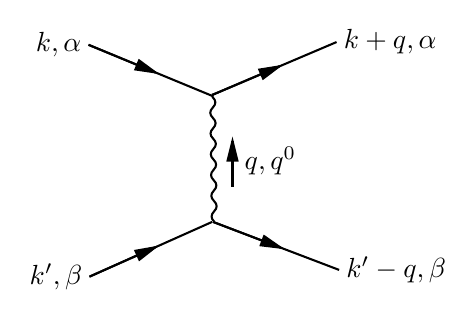
\begin{tikzpicture}[x=0.75pt,y=0.75pt,yscale=-1,xscale=1]
            %Straight Lines [id:da15915538235750892] 
            \draw    (100.17,172.51) -- (131.95,158.32) ;
            \draw [shift={(133.77,157.5)}, rotate = 515.9300000000001] [fill={rgb, 255:red, 0; green, 0; blue, 0 }  ][line width=0.08]  [draw opacity=0] (12,-3) -- (0,0) -- (12,3) -- cycle    ;
            %Straight Lines [id:da595892295722313] 
            \draw    (100.17,172.51) -- (159.26,146.12) ;
            
            %Straight Lines [id:da41375516068648066] 
            \draw    (160.29,146.04) .. controls (158.6,144.39) and (158.57,142.73) .. (160.22,141.04) .. controls (161.87,139.35) and (161.85,137.69) .. (160.16,136.04) .. controls (158.47,134.39) and (158.45,132.73) .. (160.1,131.04) .. controls (161.74,129.35) and (161.72,127.69) .. (160.03,126.04) .. controls (158.34,124.39) and (158.32,122.73) .. (159.97,121.04) .. controls (161.62,119.35) and (161.6,117.69) .. (159.91,116.04) .. controls (158.22,114.39) and (158.2,112.73) .. (159.84,111.04) .. controls (161.49,109.35) and (161.47,107.69) .. (159.78,106.04) .. controls (158.09,104.39) and (158.07,102.73) .. (159.72,101.04) .. controls (161.36,99.35) and (161.34,97.69) .. (159.65,96.04) .. controls (157.96,94.39) and (157.94,92.73) .. (159.59,91.04) .. controls (161.24,89.35) and (161.22,87.69) .. (159.53,86.04) -- (159.51,84.35) -- (159.51,84.35) ;
            %Straight Lines [id:da18427908684914152] 
            \draw    (159.7,146.12) -- (192.38,158.57) ;
            \draw [shift={(194.25,159.28)}, rotate = 200.85] [fill={rgb, 255:red, 0; green, 0; blue, 0 }  ][line width=0.08]  [draw opacity=0] (12,-3) -- (0,0) -- (12,3) -- cycle    ;
            %Straight Lines [id:da5517253733622631] 
            \draw    (159.7,146.12) -- (220.46,169.26) ;
            
            %Straight Lines [id:da9982758254698763] 
            \draw    (99.72,60.8) -- (131.97,74.12) ;
            \draw [shift={(133.82,74.88)}, rotate = 202.44] [fill={rgb, 255:red, 0; green, 0; blue, 0 }  ][line width=0.08]  [draw opacity=0] (12,-3) -- (0,0) -- (12,3) -- cycle    ;
            %Straight Lines [id:da26812450354509565] 
            \draw    (99.72,60.8) -- (159.69,85.57) ;
            
            %Straight Lines [id:da1756933542309722] 
            \draw    (159.57,84.84) -- (191.65,71.2) ;
            \draw [shift={(193.49,70.41)}, rotate = 516.96] [fill={rgb, 255:red, 0; green, 0; blue, 0 }  ][line width=0.08]  [draw opacity=0] (12,-3) -- (0,0) -- (12,3) -- cycle    ;
            %Straight Lines [id:da7638586957076614] 
            \draw    (159.57,84.84) -- (219.22,59.47) ;
            
            %Straight Lines [id:da9798265876333652] 
            \draw    (169.09,129.1) -- (169.09,107.04) ;
            \draw [shift={(169.09,105.04)}, rotate = 450] [fill={rgb, 255:red, 0; green, 0; blue, 0 }  ][line width=0.08]  [draw opacity=0] (12,-3) -- (0,0) -- (12,3) -- cycle    ;
            
            % Text Node
            \draw (97.72,60.8) node [anchor=east] [inner sep=0.75pt]    {$\boldsymbol{k} ,\alpha $};
            % Text Node
            \draw (221.22,59.47) node [anchor=west] [inner sep=0.75pt]    {$\boldsymbol{k} +\boldsymbol{q} ,\alpha $};
            % Text Node
            \draw (173.48,108.5) node [anchor=north west][inner sep=0.75pt]    {$\boldsymbol{q}, \ii q^0$};
            % Text Node
            \draw (98.17,172.51) node [anchor=east] [inner sep=0.75pt]    {$\boldsymbol{k} ',\beta $};
            % Text Node
            \draw (222.46,169.26) node [anchor=west] [inner sep=0.75pt]    {$\boldsymbol{k} '-\boldsymbol{q} ,\beta $};
            \end{tikzpicture}
    \end{gathered} = \frac{1}{V} \frac{4\pi e^2}{\abs*{\vb*{q}}^2},
\end{equation}
由于是前向散射,入射出射准粒子动量不变,虚线上没有三维动量交换,松原频率交换由于是瞬时相互作用也为零。
它给出的全部正规自能图可以概括为
\begin{equation}
    - \Sigma = \begin{gathered}
        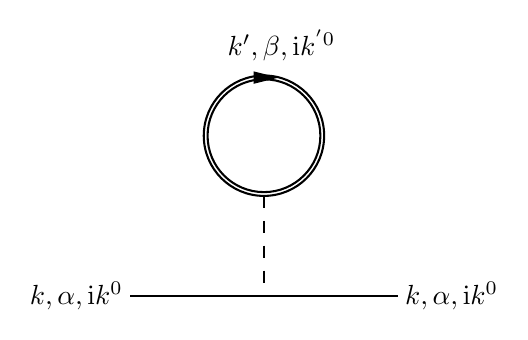
\begin{tikzpicture}[x=0.75pt,y=0.75pt,yscale=-1,xscale=1]
            %uncomment if require: \path (0,300); %set diagram left start at 0, and has height of 300
            
            %Straight Lines [id:da21065414652163694] 
            \draw    (226.85,232) -- (355.85,232) ;
            %Straight Lines [id:da10375589245043493] 
            \draw  [dash pattern={on 4.5pt off 4.5pt}]  (291.35,183.98) -- (291.35,232) ;
            %Shape: Circle [id:dp49575130445920723] 
            \draw   (262.35,154.98) .. controls (262.35,138.96) and (275.34,125.98) .. (291.35,125.98) .. controls (307.37,125.98) and (320.35,138.96) .. (320.35,154.98) .. controls (320.35,171) and (307.37,183.98) .. (291.35,183.98) .. controls (275.34,183.98) and (262.35,171) .. (262.35,154.98) -- cycle ;
            %Straight Lines [id:da49696357001991487] 
            \draw    (298.35,126.98) ;
            \draw [shift={(298.35,126.98)}, rotate = 180] [fill={rgb, 255:red, 0; green, 0; blue, 0 }  ][line width=0.08]  [draw opacity=0] (12,-3) -- (0,0) -- (12,3) -- cycle    ;
            %Shape: Circle [id:dp3232390185153] 
            \draw   (264.18,154.98) .. controls (264.18,139.97) and (276.34,127.8) .. (291.35,127.8) .. controls (306.36,127.8) and (318.53,139.97) .. (318.53,154.98) .. controls (318.53,169.99) and (306.36,182.16) .. (291.35,182.16) .. controls (276.34,182.16) and (264.18,169.99) .. (264.18,154.98) -- cycle ;
            
            % Text Node
            \draw (224.85,232) node [anchor=east] [inner sep=0.75pt]    {$\boldsymbol{k} ,\alpha ,\mathrm{i} k^{0}$};
            % Text Node
            \draw (357.85,232) node [anchor=west] [inner sep=0.75pt]    {$\boldsymbol{k} ,\alpha ,\mathrm{i} k^{0}$};
            % Text Node
            \draw (327.17,111.51) node [anchor=east] [inner sep=0.75pt]    {$\boldsymbol{k} ',\beta ,\mathrm{i} k^{'0}$};
            \end{tikzpicture}                       
    \end{gathered} = \sum_{\beta, \vb*{k}'} (-1) \times \frac{1}{V} f_{\alpha \beta \vb*{k} \vb*{k}'} \expval*{\var{n_{\vb*{k}' \beta}}},
\end{equation}
其中闭合电子回线意味着$\ii \omega_n = 0$,$-1$因子是相互作用顶角上的,闭合费米子回线由于给出了$\expval*{c^\dagger c}$,不贡献$-1$因子;
因此加入了自能修正的单粒子能量就是
\begin{equation}
    \epsilon_{\vb*{k} \alpha} = \epsilon_{\vb*{k}}^0 + \frac{1}{V} \sum_{\beta, \vb*{k}'} f_{\alpha \beta \vb*{k} \vb*{k}'} \expval*{\var{n_{\vb*{k}' \beta}}}.
    \label{eq:fermi-liquid-single-energy}
\end{equation}
期望值$\expval*{n_{\vb*{k}' \beta}}$是考虑了\eqref{eq:fermi-liquid-energy}中第二项\emph{之后}的,本身不容易直接算出,它将被用于做自洽计算。
实际上也可以更加直观地得到\eqref{eq:fermi-liquid-single-energy}:$\epsilon_{\vb*{k} \alpha}$大体上是向费米液体基态打入一个新准粒子后的能量,那让$E$对$n_{\vb*{k} \alpha}$求导就是了。

现在列写玻尔兹曼方程。设单粒子分布函数为$n_{\vb*{k} \alpha}(\vb*{r}, t)$%
\footnote{
    其实$\vb*{r}$和$\vb*{k}$的不对易比较明显时,也可以定义单粒子分布函数的,只不过此时它是Wigner函数,是单粒子密度矩阵做了一个傅里叶变换而得到的;在$\vb*{r}$和$\vb*{k}$的不对易性不明显时,经典概率分布函数、Wigner函数、密度矩阵基本上就是一回事,我们也就不再区分它们。
}%
,玻尔兹曼方程为
\begin{equation}
    \pdv{n_{\vb*{k} \alpha}}{t} + \pdv{n_{\vb*{k} \alpha}}{\vb*{r}} \cdot \pdv{\epsilon_{\vb*{k} \alpha}}{\vb*{k}} + \pdv{n_{\vb*{k} \alpha}}{\vb*{k}} \cdot \left( \vb*{F} - \pdv{\epsilon_{\vb*{k} \alpha}}{\vb*{r}} \right) = I[n_{\vb*{k} \alpha}]. 
    \label{eq:landau-fermi-liquid-equation}
\end{equation}
这个方程形式上和普通的玻尔兹曼方程一样,但是$\epsilon$和$n$之间存在关系\eqref{eq:fermi-liquid-single-energy}。
注意此时$\epsilon_{\vb*{k} \alpha}$也有$\vb*{r}$的依赖,且\eqref{eq:fermi-liquid-single-energy}中的二次量子化粒子数算符$\var{n_{\vb*{k}' \beta}}$被单粒子分布函数偏离平衡态的量$\var{n_{\vb*{k}' \beta}}$取代,即此时我们就只需要写出
\begin{equation}
    \epsilon_{\vb*{k} \alpha} = \epsilon_{\vb*{k}}^0 + \frac{1}{V} \sum_{\beta, \vb*{k}'} f_{\alpha \beta \vb*{k} \vb*{k}'} \var{n_{\vb*{k}' \beta}}.
    \label{eq:fermi-liquid-single-energy-kinetic}
\end{equation}
有时我们将\eqref{eq:landau-fermi-liquid-equation}联立上\eqref{eq:fermi-liquid-single-energy-kinetic}称为\concept{朗道方程}。
朗道动理学方程的稳态或者说费米液体的热力学基态当然形式上和费米气体是完全一样的,是
\begin{equation}
    n_{\vb*{k} \alpha} = \frac{1}{\ee^{\beta \epsilon_{\vb*{k} \alpha}} + 1},
    \label{eq:fermi-liquid-stable-state}
\end{equation}
但同样需要联立\eqref{eq:fermi-liquid-single-energy}才能求解。

\subsubsection{费米液体中的集体振荡模式}

由于动理学方程实际上是准粒子二体格林函数的运动方程的一个近似,它给出的$n_{\vb*{k} \alpha}$如果随着时间有某种振荡模式,做完傅里叶变换就会有极点,即存在一个准粒子集体运动形成的元激发。
通过分析动理学方程的稳定周期解,就能够找到很大一类费米液体中的元激发。

我们采用弛豫时间近似,即
\begin{equation}
    \pdv{n_{\vb*{k} \alpha}}{t} + \pdv{n_{\vb*{k} \alpha}}{\vb*{r}} \cdot \pdv{\epsilon_{\vb*{k} \alpha}}{\vb*{k}} + \pdv{n_{\vb*{k} \alpha}}{\vb*{k}} \cdot \left( \vb*{F} - \pdv{\epsilon_{\vb*{k} \alpha}}{\vb*{r}} \right) = - \frac{n_{\vb*{k} \alpha} - n_{\vb*{k} \alpha}^0}{\tau},
    \label{eq:landau-equation-damping}
\end{equation}
由于弛豫是粒子碰撞导致的,$\tau \propto T^{-2}$。注意\eqref{eq:landau-fermi-liquid-equation}的碰撞项中是\emph{没有}温度依赖的,并且大体上正比于$n_{\vb*{k} \alpha}$的平方;然而,$n_{\vb*{k} \alpha}$本身是有温度依赖的,在系统偏离平衡态不多时,可以将碰撞项写成$n_{\vb*{k} \alpha} / \tau$这样的弛豫项,此时的$\tau$就是有温度依赖的。

系统状态偏离平衡态首先会导致的就是\eqref{eq:fermi-liquid-single-energy-kinetic}中的$n$不再是由\eqref{eq:fermi-liquid-stable-state}和\eqref{eq:fermi-liquid-single-energy-kinetic}联合确定的那个费米分布状态,然后玻尔兹曼方程\eqref{eq:landau-equation-damping}又会根据\eqref{eq:fermi-liquid-single-energy-kinetic}算出的$\epsilon$改变$n$。
我们采取如下求解策略:设${n}^0_{\vb*{k} \alpha}$为将实际的(暂时还不确定的)${n}_{\vb*{k} \alpha}$代入\eqref{eq:fermi-liquid-single-energy-kinetic},将得到的真实$\epsilon_{\vb*{k} \alpha}$代入\eqref{eq:fermi-liquid-stable-state}右边计算出来的分布函数,然后将$\hat{n}_{\vb*{k}}$在$\hat{n}^0_{\vb*{k}}$附近展开到平衡态附近的一阶(由于只考虑近平衡态),得到将\eqref{eq:landau-equation-damping}线性化的关于
\begin{equation}
    \var{n_{\vb*{k} \alpha}} = n_{\vb*{k} \alpha} - n_{\vb*{k} \alpha}^0
\end{equation}
的演化方程。
注意到$n_{\vb*{k} \alpha}^0$不依赖于时间和坐标,而$\epsilon_{\vb*{k} \alpha}$不依赖于坐标,仅保留正比于$\var{n}_{\vb*{k} \alpha}$的项,得到
\begin{equation}
    \pdv{\var{n}_{\vb*{k} \alpha}}{t} + \pdv{\epsilon^0_{\vb*{k} \alpha}}{\vb*{k}} \cdot \pdv{\var{n_{\vb*{k} \alpha}}}{\vb*{r}} - \pdv{n^0_{\vb*{k} \alpha}}{\vb*{k}} \cdot \pdv{\var{\epsilon_{\vb*{k} \alpha}}}{\vb*{r}} = - \frac{\var{n}_{\vb*{k} \alpha}}{\tau}.
    \label{eq:delta-from-stable-fermi-liquid}
\end{equation}

\eqref{eq:landau-equation-damping}描述的系统中能够传播的波大致上可以分成两种,一种是普通的声波,一种是所谓的零声。
设波动的圆频率为$\omega$,如果$\omega \tau \ll 1$,那么准静态近似成立,即有波动传递的费米液体的每一点几乎都是热力学平衡的。
弛豫项$n_{\vb*{k} \alpha} / \tau$起到的作用主要是把准粒子分布“拖”向平衡态。
这样的波动就是普通的声波(虽然寻常的传递声波的液体中的粒子没有费米统计而费米液体中的粒子有,但两者都可以在适当的情况下使用玻尔兹曼方程描述,从而都有声波)。%
$\omega \tau$稍微大一些时,准静态近似不再成立,在热力学上这意味着会有明显的熵产生,换句话说,在费米液体中激发出的任何振动模式都会快速因为碰撞而受到阻尼,没有能够稳定传播的模式。
在温度非常低时,基本上没有声波能够传递。这是正确的,因为声波的传播需要准粒子碰撞,而温度非常低时没有什么碰撞事件发生。%
\footnote{
    这里“零温”一词可能引起混淆;我们\emph{不是}说普通声波是一个纯粹有限温的现象——它当然可以在纯态(“零温”)系统中发生。
    但是,对处在\emph{热态}中而温度为零(另一种“零温”)的系统——即状态和费米球相差不大的系统——声波是很难产生的。
}%

但这并不是说$T \to 0$时费米液体中没有任何集体振动模式。
当$\omega \tau \gg 1$时,一幅非常奇怪的图景出现了:此时弛豫项几乎可以忽略,因此,外界扰动而产生的$n_{\vb*{k} \alpha}$涨落传播到的地方\emph{不会}发生任何弛豫现象,无法达到热平衡,且波动\emph{不会}受到任何阻尼。
此时的波动称为\concept{零声},因为它看起来很像声波,但首先频率通常高于普通的声波,其次通常需要$\tau$比较大才能观察到,即需要在非常接近绝对零度的系统中才能观察到。

\subsection{零声}

\subsubsection{费米液体在绝对零度的低能激发}

\begin{figure}
    \centering
    \subfigure[变形的费米面,费米液体在$T=0$时的低能激发普遍具有这个形式]{
        

\tikzset{every picture/.style={line width=0.75pt}} %set default line width to 0.75pt        

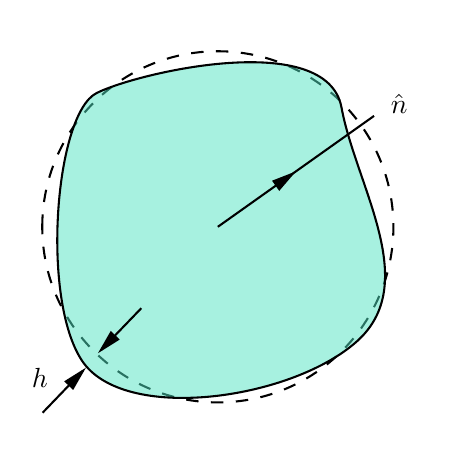
\begin{tikzpicture}[x=0.75pt,y=0.75pt,yscale=-1,xscale=1]
%uncomment if require: \path (0,300); %set diagram left start at 0, and has height of 300

%Shape: Circle [id:dp01917491317166009] 
\draw  [dash pattern={on 4.5pt off 4.5pt}] (121.52,175.11) .. controls (121.52,128.4) and (159.4,90.52) .. (206.11,90.52) .. controls (252.83,90.52) and (290.71,128.4) .. (290.71,175.11) .. controls (290.71,221.83) and (252.83,259.71) .. (206.11,259.71) .. controls (159.4,259.71) and (121.52,221.83) .. (121.52,175.11) -- cycle ;
%Shape: Polygon Curved [id:ds19124968571483536] 
\draw  [fill={rgb, 255:red, 80; green, 227; blue, 194 }  ,fill opacity=0.5 ] (147.71,110.66) .. controls (167.71,100.66) and (258.71,79.66) .. (265.71,117.66) .. controls (272.71,155.66) and (304.71,202.66) .. (272.71,230.66) .. controls (240.71,258.66) and (160.71,269.66) .. (140.71,239.66) .. controls (120.71,209.66) and (127.71,120.66) .. (147.71,110.66) -- cycle ;
%Straight Lines [id:da9840179317331423] 
\draw    (206.11,175.11) -- (281.38,121.67) ;
\draw [shift={(243.75,148.39)}, rotate = 504.62] [fill={rgb, 255:red, 0; green, 0; blue, 0 }  ][line width=0.08]  [draw opacity=0] (12,-3) -- (0,0) -- (12,3) -- cycle    ;
%Straight Lines [id:da9902953526542171] 
\draw    (121.71,264.66) -- (141.19,244.42) ;
\draw [shift={(142.58,242.98)}, rotate = 493.92] [fill={rgb, 255:red, 0; green, 0; blue, 0 }  ][line width=0.08]  [draw opacity=0] (12,-3) -- (0,0) -- (12,3) -- cycle    ;
%Straight Lines [id:da6416680662048091] 
\draw    (169.25,214.31) -- (149.76,234.55) ;
\draw [shift={(148.37,235.99)}, rotate = 313.91999999999996] [fill={rgb, 255:red, 0; green, 0; blue, 0 }  ][line width=0.08]  [draw opacity=0] (12,-3) -- (0,0) -- (12,3) -- cycle    ;

% Text Node
\draw (115,242) node [anchor=north west][inner sep=0.75pt]    {$h$};
% Text Node
\draw (287.96,109.72) node [anchor=north west][inner sep=0.75pt]    {$\hat{n}$};


\end{tikzpicture}

    }
    \caption{费米面的变形和零声}
\end{figure}


我们来计算$T=0$时的零声模式,实际上就是要处理$T=0$时的费米液体的低能激发。
此时\eqref{eq:delta-from-stable-fermi-liquid}右边为零。
我们考虑一个$f_{\alpha \beta \vb*{k} \vb*{k}'}$中无自旋依赖的系统,因为与自旋相关的那种涨落通常称为自旋密度波。
为方便起见我们将$\vb*{k}$给定而携带一个自旋指标的分布函数记作$\hat{n}_{\vb*{k}}$,同理$f$记作$\hat{f}_{\vb*{k} \vb*{k}'}$。

我们有
\[
    \pdv{\hat{n}^0_{\vb*{k}}}{\vb*{k}} = - \delta(\epsilon_{\vb*{k}} - \epsilon_\text{F}) \vb*{v}, \quad  \pdv{\epsilon_{\vb*{k}}^0}{\vb*{k}} \approx \vb*{v}, \quad \var{\epsilon_{\vb*{k}}} = \frac{1}{V} \Trace' \sum_{\vb*{k}'} \hat{f}_{\vb*{k} \vb*{k}'} \var{\hat{n}_{\vb*{k}'}} = \Trace' \int \frac{\dd[3]{\vb*{k}'}}{(2\pi)^3} \hat{f}_{\vb*{k} \vb*{k}'} \var{\hat{n}_{\vb*{k}'}},
\]
这里我们使用惯常的群速度定义
\begin{equation}
    \vb*{v} = \pdv{\epsilon_{\vb*{k}}}{\vb*{k}} \approx \pdv{\epsilon^0_{\vb*{k}}}{\vb*{k}} = \frac{\vb*{k}}{m^*} \approx v_\text{F} \vu*{k},
\end{equation}
因此$\vb*{v}$和$\vb*{k}$的指向是一致的,记它们的指向为$\vu*{n}$。
这样,\eqref{eq:delta-from-stable-fermi-liquid}化为
\begin{equation}
    \pdv{\var{\hat{n}_{\vb*{k}}}}{t} + \vb*{v} \cdot \pdv{\var{\hat{n}_{\vb*{k}}}}{\vb*{r}} + \delta(\epsilon_{\vb*{k}} - \epsilon_\text{F}) \vb*{v} \cdot \Trace' \int \frac{\dd[3]{\vb*{k}'}}{(2\pi)^3} \hat{f}_{\vb*{k} \vb*{k}'} \pdv{\var{\hat{n}_{\vb*{k}'}}}{\vb*{r}} = 0.
    \label{eq:original-nu-equation-fermi-liquid}
\end{equation}
注意到上式具有时间和空间平移不变性,即可以做傅里叶变换,且第三项中的$\delta(\epsilon_{\vb*{k}} - \epsilon_\text{F})$无法通过对$\vb*{r}$或是$t$求导得到,于是不失一般性地,可以$\var{\hat{n}_{\vb*{k}}}$具有以下形式
\[
    \var{\hat{n}_{\vb*{k}}} = \ee^{\ii (\vb*{q} \cdot \vb*{r} - \omega t)} \delta(\epsilon_{\vb*{k}} - \epsilon_\text{F}) \hat{\nu}_{\vb*{k}},
\]
$\omega$和$\vb*{q}$分别是零声的频率和波矢,$\hat{\nu}$不依赖于$\vb*{r}$。
此外,由于我们只关心费米面附近的行为,可以认为$\vb*{k}$提供的信息主要是关于其指向而不是其大小的(大小就是$k_\text{F}$;由于\eqref{eq:original-nu-equation-fermi-liquid}中没有对$\vb*{k}$的导数,无需考虑费米面附近$\var{\hat{n}_{\vb*{k}}}$的变化趋势),从而
\begin{equation}
    \var{\hat{n}_{\vb*{k}}}(\vb*{r}) = \ee^{\ii (\vb*{q} \cdot \vb*{r} - \omega t)} \delta(\epsilon_{\vb*{k}} - \epsilon_\text{F}) \hat{\nu}(\vu*{n}).
    \label{eq:zero-sound-distribution-form}
\end{equation}
注意\eqref{eq:original-nu-equation-fermi-liquid}中$\vb*{r}$具有空间各向同性而$\vb*{k}$未必具有($f$可以破坏动量空间的各向同性)。

\eqref{eq:original-nu-equation-fermi-liquid}的形式看起来很奇怪,不过实际上这说明费米液体中如果有波矢为$\vb*{q}$,频率为$\omega$的零声存在,那么仍然有一个费米面,只不过费米面的形状发生了扭曲。
我们反过来论证这件事。$T=0$时的分布函数满足
\[
    \var{\hat{n}} \propto \theta(\epsilon_{\vb*{k}} - \epsilon_\text{F}) \approx \theta\left( \frac{k_\text{F}}{m^*} (k(\vu*{n}) - k_\text{F}) \right),
\]
设费米面在方向$\vu*{n}$上发生了按照动量来说,大小为$h(\vu*{n})$的位移,则此时的分布函数为
\[
    \hat{n} \propto \theta\left( \frac{k_\text{F}}{m^*} (k(\vu*{n}) - k_\text{F} - h(\vu*{n})) \right) \approx \theta(\epsilon_{\vb*{k}} - \epsilon_\text{F}) + \frac{k_\text{F}}{m^*} \delta(\epsilon_{\vb*{k}} - \epsilon_\text{F}) h(\vu*{n}),
\]
即
\[
    \var{\hat{n}} \propto \delta(\epsilon_{\vb*{k}} - \epsilon_\text{F}) h(\vu*{n}).
\]
这和\eqref{eq:zero-sound-distribution-form}的形式完全一样,因此$\hat{\nu}(\vu*{n})$其实给出了费米面偏移的多少。

\begin{figure}
    \centering
    

\tikzset{every picture/.style={line width=0.75pt}} %set default line width to 0.75pt        

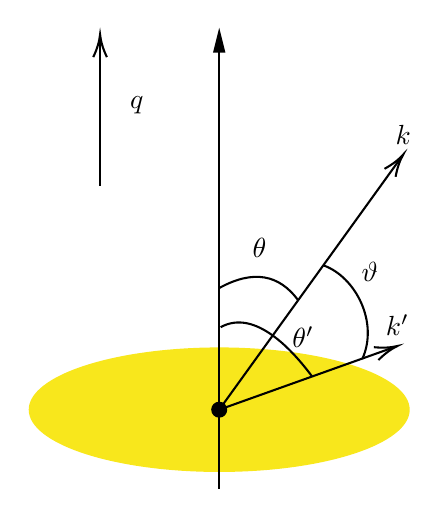
\begin{tikzpicture}[x=0.75pt,y=0.75pt,yscale=-1,xscale=1]
%uncomment if require: \path (0,300); %set diagram left start at 0, and has height of 300

%Shape: Ellipse [id:dp004925494082220538] 
\draw  [draw opacity=0][fill={rgb, 255:red, 248; green, 231; blue, 28 }  ,fill opacity=1 ] (103.22,202.78) .. controls (103.22,186.21) and (144.31,172.78) .. (195,172.78) .. controls (245.69,172.78) and (286.78,186.21) .. (286.78,202.78) .. controls (286.78,219.34) and (245.69,232.78) .. (195,232.78) .. controls (144.31,232.78) and (103.22,219.34) .. (103.22,202.78) -- cycle ;
%Straight Lines [id:da570355407153736] 
\draw    (195,240.78) -- (195,20.78) ;
\draw [shift={(195,18.78)}, rotate = 450] [fill={rgb, 255:red, 0; green, 0; blue, 0 }  ][line width=0.08]  [draw opacity=0] (12,-3) -- (0,0) -- (12,3) -- cycle    ;
%Straight Lines [id:da0346655085632539] 
\draw    (137.6,23.98) -- (137.6,95.2) ;
\draw [shift={(137.6,21.98)}, rotate = 90] [color={rgb, 255:red, 0; green, 0; blue, 0 }  ][line width=0.75]    (10.93,-3.29) .. controls (6.95,-1.4) and (3.31,-0.3) .. (0,0) .. controls (3.31,0.3) and (6.95,1.4) .. (10.93,3.29)   ;
%Straight Lines [id:da927413661316274] 
\draw    (195,202.78) -- (282.54,81.4) ;
\draw [shift={(283.71,79.78)}, rotate = 485.8] [color={rgb, 255:red, 0; green, 0; blue, 0 }  ][line width=0.75]    (10.93,-3.29) .. controls (6.95,-1.4) and (3.31,-0.3) .. (0,0) .. controls (3.31,0.3) and (6.95,1.4) .. (10.93,3.29)   ;
%Straight Lines [id:da8188066243539127] 
\draw    (195,202.78) ;
\draw [shift={(195,202.78)}, rotate = 0] [color={rgb, 255:red, 0; green, 0; blue, 0 }  ][fill={rgb, 255:red, 0; green, 0; blue, 0 }  ][line width=0.75]      (0, 0) circle [x radius= 3.35, y radius= 3.35]   ;
%Straight Lines [id:da07180626735433826] 
\draw    (195,202.78) -- (279.01,172.76) ;
\draw [shift={(280.89,172.08)}, rotate = 520.3399999999999] [color={rgb, 255:red, 0; green, 0; blue, 0 }  ][line width=0.75]    (10.93,-3.29) .. controls (6.95,-1.4) and (3.31,-0.3) .. (0,0) .. controls (3.31,0.3) and (6.95,1.4) .. (10.93,3.29)   ;
%Curve Lines [id:da9617442437621511] 
\draw    (194.89,144.23) .. controls (211.6,135.01) and (223.89,137.83) .. (232.89,149.83) ;
%Curve Lines [id:da2265273671127297] 
\draw    (195.69,163.03) .. controls (212.4,153.81) and (230.69,174.68) .. (239.69,186.68) ;
%Curve Lines [id:da702403488804388] 
\draw    (245.53,133.36) .. controls (260.73,138.96) and (271.93,160.76) .. (263.93,178.36) ;

% Text Node
\draw (160.04,56.2) node [anchor=east] [inner sep=0.75pt]    {$\boldsymbol{q}$};
% Text Node
\draw (283.71,76.38) node [anchor=south] [inner sep=0.75pt]    {$\boldsymbol{k}$};
% Text Node
\draw (280.89,168.68) node [anchor=south] [inner sep=0.75pt]    {$\boldsymbol{k} '$};
% Text Node
\draw (209.6,118.8) node [anchor=north west][inner sep=0.75pt]    {$\theta $};
% Text Node
\draw (228.8,161.2) node [anchor=north west][inner sep=0.75pt]    {$\theta '$};
% Text Node
\draw (262.12,130.14) node [anchor=north west][inner sep=0.75pt]    {$\vartheta $};


\end{tikzpicture}

    \caption{计算过程中建立的坐标系,$\theta$和$\theta'$是$\vb*{k}$和$\vb*{k}'$的极角,$\vartheta$是这两者之间的夹角}
\end{figure}

将\eqref{eq:zero-sound-distribution-form}代入\eqref{eq:original-nu-equation-fermi-liquid},得到
\[
    (\omega - \vb*{v} \cdot \vb*{q}) \hat{\nu}(\vu*{n}) = \vb*{v} \cdot \vb*{q} \Trace' \int \frac{\dd[3]{\vb*{k}'}}{(2\pi)^3} \hat{f}_{\vb*{k} \vb*{k}'} \delta(\epsilon_{\vb*{k}'} - \epsilon_\text{F}) \hat{\nu}(\vu*{n}').
\]
上式右边只和$\vb*{k}'$在费米面附近处时$f_{\vb*{k} \vb*{k}'}$的值有关,我们不妨设$\vb*{k}$和$\vb*{k}'$均在费米面附近的$f_{\vb*{k} \vb*{k}'}$为$f(\vu*{n}, \vu*{n}')$,则有
\[
    \begin{aligned}
        \Trace' \int \frac{\dd[3]{\vb*{k}'}}{(2\pi)^3} \hat{f}_{\vb*{k} \vb*{k}'} \delta(\epsilon_{\vb*{k}'} - \epsilon_\text{F}) \hat{\nu}(\vu*{n}') &= \frac{1}{(2\pi)^3} \Trace' \int k_\text{F}^2 \dd{\Omega'} \frac{1}{\abs{\pdv{\epsilon_{\vb*{k}}}{\vb*{k}}}} \hat{f}(\vu*{n}, \vu*{n}') \hat{\nu}(\vu*{n}'),
    \end{aligned}
\]
因此
\[
    (\omega - v_\text{F} \vu*{n} \cdot \vb*{q}) \hat{\nu}(\vu*{n}) = \vu*{n} \cdot \vb*{q} \frac{k_\text{F}^2}{(2\pi)^3} \Trace' \int \dd{\Omega'} \hat{f}(\vu*{n}, \vu*{n}') \hat{\nu}(\vu*{n}').
\]
现在将上式两边取$\Trace$运算,有
\[
    (\omega - v_\text{F} \vu*{n} \cdot \vb*{q}) {\nu}(\vu*{n}) = \vu*{n} \cdot \vb*{q} \frac{k_\text{F}^2}{(2\pi)^3} \Trace \Trace' \int \dd{\Omega'} \hat{f}(\vu*{n}, \vu*{n}') \hat{\nu}(\vu*{n}'),
\]
这里$\nu(\vu*{n}) = \Trace \hat{\nu}(\vu*{n})$,而从\eqref{eq:fermi-liquid-f-sym-decomposition}会发现
\[
    \Trace \Trace' \hat{f}(\vu*{n}, \vu*{n}') \hat{\nu}(\vu*{n}') = \frac{2 \pi^2}{k_\text{F} m^*} F^\text{S}(\vartheta) \nu(\vu*{n}'),
\]
于是
\begin{equation}
    (\omega - v_\text{F} \vu*{n} \cdot \vb*{q}) {\nu}(\vu*{n}) = \vb*{q} \cdot \vu*{n} v_\text{F} \int \frac{\dd{\Omega}'}{4\pi} F^\text{S}(\vartheta) \nu(\vu*{n}').
\end{equation}
现在以$\vb*{q}$的方向为$z$轴,建立球坐标系以确定$\vu*{n}$的方向,记
\begin{equation}
    u_0 = \omega / \abs{\vb*{q}}, \quad s = u_0 / v_\text{F},
\end{equation}
就有
\begin{equation}
    (s - \cos \theta) \nu(\theta, \varphi) = \cos \theta \int \frac{\dd{\Omega'}}{4\pi} F^\text{S}(\vartheta) \nu(\theta', \varphi').
    \label{eq:fermi-liquid-nu-determine}
\end{equation}
在$\vb*{q}$给定后,求解此积分方程(这实际上是一个本征值问题)即可得到$\nu(\vu*{n})$和$\omega$。

在$s \leq 1$时$v(\theta, \varphi)$是有极点的,于是\eqref{eq:fermi-liquid-nu-determine}右边的积分中也是有极点的,因此积分路径在复平面上必定需要用某种方式绕过该极点,则\eqref{eq:fermi-liquid-nu-determine}的左右两边都会出现虚部,因此$\omega$有虚部,因此零声存在衰减。

% TODO:切伦科夫辐射,朗道阻尼,等等

\subsubsection{零声模式和能谱}

我们来分析一些常见情况下的零声模式和能谱。首先考虑$F^\text{S}(\vartheta)$各向同性的情况,即\eqref{eq:fermi-liquid-f-l}中只有$l=0$的分量的情况。
此时\eqref{eq:fermi-liquid-nu-determine}右边的积分没有$\theta$和$\varphi$的依赖,因此左边也没有,因此
\begin{equation}
    \nu(\theta, \varphi) = \const \times \frac{\cos \theta}{s - \cos \theta},
    \label{eq:round-fermi-ball-oscillation}
\end{equation}
这是一个各向异性的振动,虽然此时费米液体的整个哈密顿量都是各向同性的。当然这没有引起任何矛盾,因为说到底这是激发态,考虑到$\vb*{q}$的方向可以任意选取,各向同性是能够保证的。
在\eqref{eq:round-fermi-ball-oscillation}知道之后,\eqref{eq:fermi-liquid-nu-determine}就等价于
\[
    1 = \int \frac{2 \pi \sin \theta' \dd{\theta'}}{4\pi} F^\text{S}_0 \frac{\cos \theta'}{s - \cos \theta'},
\]
也即
\begin{equation}
    \frac{s}{2} \ln\frac{s+1}{s-1} - 1 = \frac{1}{F^\text{S}_0}.
\end{equation}
因此$F^\text{S}_0$给定后$s$是常数,因此零声是线性色散的。

\subsubsection{流体动力学化}

请注意$n_{\vb*{k} \sigma}$本身是粒子数的期望的某种经典化,而粒子数期望的严格运动方程是所谓Schwinger-Dyson方程。
因此,朗道方程\eqref{eq:landau-fermi-liquid-equation}——实际上就是粒子数的经典运动方程——和粒子数期望的严格运动方程之间实际上只相差一些由于交换算符而产生的$\delta$函数项,通常这意味着粒子数\emph{算符}满足的海森堡绘景运动方程的形式和零温朗道方程是一样的。
由于朗道方程代入$\epsilon_{\vb*{k} \alpha}$的定义之后是自洽的,这实际上是说,我们可以通过朗道方程\eqref{eq:landau-fermi-liquid-equation}就得到只关于朗道费米液体的密度涨落的等效哈密顿量,而且是货真价实的、是算符的、做了勒让德变换之后能够出现在路径积分中的哈密顿量。
对那些只有密度涨落才是重要的的系统,实际上我们确实只需要密度涨落的等效哈密顿量。
因此通过观察\eqref{eq:landau-fermi-liquid-equation},我们实际上可以将费米液体玻色化。

由于严格满足费米液体的第二条假设的系统只要求系统不偏离基态太远,\eqref{eq:landau-equation-damping}费米液体

\subsection{费米液体理论的合理性}

费米液体的合理性实际上仍然不是特别明确,主要是因为我们还无法确定什么时候费米液体理论就不适用了,自然也无法确定何时费米液体确实适用。
确定一个系统是否适用费米液体理论首先需要我们确定系统的低能激发是否真的与电子的行为类似,因为原则上完全可以出现诸如电子配对等现象,或者自旋电荷分离,等等。
这件事一般来说是非常困难的,因为直接从相互作用电子气出发做微扰计算得到的当然是修正后的电子,即严格地判断系统的低能激发到底是什么多少需要一些非微扰的方法。

在确定系统的低能激发和电子行为类似之后,费米球的存在性,以及低能激发主要是费米面附近的准粒子和空穴就可以确定。
此时需要讨论的主要是相互作用的类型,即是否前向散射占据主要地位。
这件事倒是不难:我们下面展示多种方法确定这一点。

\subsubsection{重整化群}

在重整化群计算中,一个二体散射项的强弱主要由这个散射项中允许的的粒子动量的取值多少确定,可能的动量占据的空间体积越大,对应的相互作用通道就越强。

懒得写了,总之就是BCS相互作用和密度-密度相互作用是特别强的两种。
% TODO:那Hubbard模型?

\subsubsection{格林函数计算}

格林函数计算也可以给费米液体理论提供一定的辩护。我们计算单电子格林函数,实际上就是要计算自能修正。
我们考虑一个任意的\eqref{eq:general-electron-electron-interaction}中的相互作用势能,考虑一圈图,两个自能图是
\begin{equation}
    - \Sigma^{\text{Hartree}}_{\vb*{k} \sigma \omega} = \begin{gathered}
        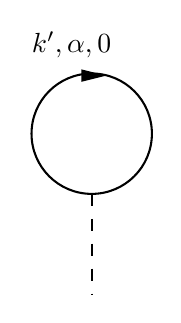
\begin{tikzpicture}[x=0.75pt,y=0.75pt,yscale=-1,xscale=1]
            %uncomment if require: \path (0,300); %set diagram left start at 0, and has height of 300
            
            %Straight Lines [id:da7796585827567135] 
            \draw  [dash pattern={on 4.5pt off 4.5pt}]  (247.35,162.98) -- (247.35,211) ;
            %Shape: Circle [id:dp5603225998122126] 
            \draw   (218.35,133.98) .. controls (218.35,117.96) and (231.34,104.98) .. (247.35,104.98) .. controls (263.37,104.98) and (276.35,117.96) .. (276.35,133.98) .. controls (276.35,150) and (263.37,162.98) .. (247.35,162.98) .. controls (231.34,162.98) and (218.35,150) .. (218.35,133.98) -- cycle ;
            %Straight Lines [id:da24340217870718206] 
            \draw    (254.35,105.98) ;
            \draw [shift={(254.35,105.98)}, rotate = 180] [fill={rgb, 255:red, 0; green, 0; blue, 0 }  ][line width=0.08]  [draw opacity=0] (12,-3) -- (0,0) -- (12,3) -- cycle    ;
            
            % Text Node
            \draw (217,83.4) node [anchor=north west][inner sep=0.75pt]    {$\boldsymbol{k} ',\alpha ,0$};
            \end{tikzpicture}      
   \end{gathered} = \frac{1}{V} \sum_{\vb*{k}', \alpha} (- V_0) n_{\vb*{k}' \alpha}^0,
   \label{eq:lowerest-self-energy-hartree-fermi-liquid}
\end{equation}
和
\begin{equation}
    \begin{gathered}
        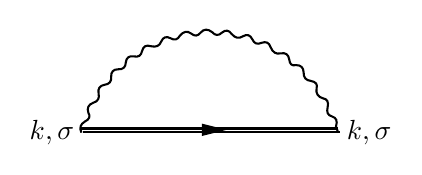
\begin{tikzpicture}[x=0.75pt,y=0.75pt,yscale=-1,xscale=1]
            %uncomment if require: \path (0,300); %set diagram left start at 0, and has height of 300
            
            %Straight Lines [id:da7649384762699059] 
            \draw    (274,238) -- (397.71,238) ;
            %Straight Lines [id:da04845933897994015] 
            \draw    (344,238.62) ;
            \draw [shift={(344,238.62)}, rotate = 180] [fill={rgb, 255:red, 0; green, 0; blue, 0 }  ][line width=0.08]  [draw opacity=0] (12,-3) -- (0,0) -- (12,3) -- cycle    ;
            %Straight Lines [id:da7745729731375024] 
            \draw    (274.74,239.78) -- (398.44,239.78) ;
            %Curve Lines [id:da11998126870239156] 
            \draw    (274,240) .. controls (272.94,237.69) and (273.5,235.91) .. (275.68,234.65) .. controls (277.88,233.56) and (278.44,232.15) .. (277.35,230.42) .. controls (276.59,228.07) and (277.36,226.47) .. (279.66,225.62) .. controls (281.95,224.93) and (282.82,223.43) .. (282.27,221.12) .. controls (281.84,218.75) and (282.81,217.35) .. (285.17,216.92) .. controls (287.5,216.65) and (288.55,215.36) .. (288.34,213.03) .. controls (288.25,210.66) and (289.39,209.47) .. (291.75,209.46) .. controls (294.06,209.59) and (295.27,208.5) .. (295.39,206.2) .. controls (295.64,203.87) and (296.92,202.88) .. (299.23,203.25) .. controls (301.46,203.75) and (302.8,202.88) .. (303.24,200.63) .. controls (303.82,198.38) and (305.21,197.61) .. (307.42,198.34) .. controls (310,198.96) and (311.68,198.2) .. (312.47,196.07) .. controls (313.39,193.94) and (314.87,193.42) .. (316.92,194.49) .. controls (318.87,195.66) and (320.38,195.24) .. (321.46,193.25) .. controls (323.21,191.18) and (325,190.84) .. (326.85,192.23) .. controls (328.58,193.69) and (330.14,193.52) .. (331.52,191.72) .. controls (333.03,189.97) and (334.85,189.92) .. (337,191.57) .. controls (338.48,193.29) and (340.05,193.37) .. (341.7,191.82) .. controls (343.47,190.34) and (345.03,190.54) .. (346.37,192.43) .. controls (348.08,194.46) and (349.88,194.84) .. (351.77,193.59) .. controls (353.78,192.42) and (355.3,192.88) .. (356.33,194.97) .. controls (357.22,197.08) and (358.71,197.66) .. (360.8,196.72) .. controls (362.99,195.9) and (364.45,196.61) .. (365.16,198.84) .. controls (366.19,201.35) and (367.83,202.33) .. (370.08,201.78) .. controls (372.42,201.37) and (373.77,202.35) .. (374.13,204.71) .. controls (374.35,207.05) and (375.43,207.96) .. (377.36,207.44) .. controls (379.78,207.43) and (381.02,208.63) .. (381.07,211.06) .. controls (381,213.46) and (382.16,214.8) .. (384.56,215.07) .. controls (387.01,215.52) and (387.92,216.73) .. (387.29,218.71) .. controls (386.92,221.16) and (387.94,222.73) .. (390.33,223.44) .. controls (392.42,223.74) and (393.2,225.15) .. (392.65,227.68) .. controls (392,230.16) and (392.71,231.66) .. (394.77,232.19) .. controls (396.84,232.82) and (397.48,234.42) .. (396.67,236.99) -- (397.71,240) ;
            
            % Text Node
            \draw (272,240) node [anchor=east] [inner sep=0.75pt]    {$\boldsymbol{k} , \sigma $};
            % Text Node
            \draw (400.44,239.78) node [anchor=west] [inner sep=0.75pt]    {$\boldsymbol{k} , \sigma$};
            \end{tikzpicture}            
    \end{gathered} = \int \frac{\dd[3]{\vb*{q}}}{(2\pi)^3} (- \expval{n_{\vb*{q} \sigma}}) \frac{- \ii 4 \pi e^2}{\abs*{\vb*{k} - \vb*{q}}^2} .
\end{equation}
它们均没有$\omega$依赖,即重整化因子$Z=1$。
因此对一个做单圈自能修正就够了的费米子系统,等效单粒子能量为
\begin{equation}
    \xi_{\vb*{k} \alpha} = \xi^0_{\vb*{k} \alpha} + \sum_{\vb*{k}', \beta} (V_0 - V_{\vb*{k} - \vb*{k}'} \delta_{\alpha \beta}) n_{\vb*{k}' \beta}^0,
\end{equation}
且单电子格林函数的形式和自由电子格林函数完全一致,区别在于要将$\xi^0_{\vb*{k} \alpha}$替换成$\xi_{\vb*{k} \alpha}$。
这就意味着,首先,重整化后电子仍然是有费米面的;其次,如果近似认为$n^0$就是$n$,\eqref{eq:fermi-liquid-energy}可以看成重整化后电子的等效哈密顿量。
这就说明相互作用电子气的低能理论就是费米液体,并且费米液体中的准粒子就是相互作用修饰后的电子。

上面的推导中没有体现出一件事:如果$n$变了,那么$\epsilon$会跟着发生变化,这在我们推导朗道方程\eqref{eq:landau-fermi-liquid-equation}并且分析其行为时体现得尤其重要。
这是因为\eqref{eq:lowerest-self-energy-hartree-fermi-liquid}和\eqref{eq:lowerest-self-energy-fock-fermi-liquid}都是最低阶的图,其中的电子线自己没有经过相互作用修饰。
完整的图——做了正确的电子自能、真空极化、相互作用顶角修饰——中的电子线给出$n_{\vb*{k} \alpha}$,因此的确如果$n$变了,那么$\epsilon$会跟着发生变化;由于真空极化、相互作用顶角修饰也依赖于$n$,此时的系统总能量实际上相比\eqref{eq:fermi-liquid-energy}还要多出来一些项。
容易看出,直接导致\eqref{eq:fermi-liquid-energy}的是自洽Hartree-Fock近似,其中自由电子线被修正为相互作用电子线(见\autoref{fig:scf-fermi-liquid}),从而$n^0$被替换成$n$。
因此费米液体理论实际上可以看成一种平均场理论。当然,从\eqref{eq:fermi-liquid-single-energy}的形式其实就可以看到这一点了。
它和凝胶模型中的自洽Hartree-Fock近似的不同之处在于$V_{\vb*{q}}$可以不是库伦排斥能,例如,可以做RPA近似得到等效屏蔽势,然后再做自洽Hartree-Fock近似。
因此费米液体理论在给定了合适的$\epsilon^0$和$f$之后能够非常精确地描述电子气的行为,而不像直接对库仑相互作用做Hartree-Fock近似一样很多时候计算不准确。

\begin{figure}
    \centering
    

\tikzset{every picture/.style={line width=0.75pt}} %set default line width to 0.75pt        

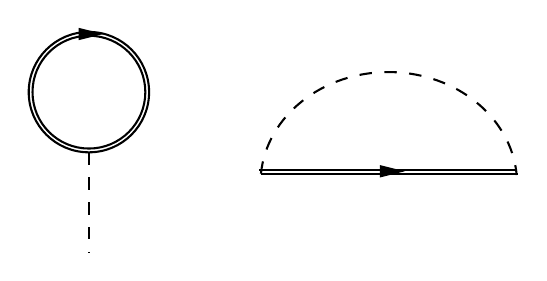
\begin{tikzpicture}[x=0.75pt,y=0.75pt,yscale=-1,xscale=1]
%uncomment if require: \path (0,300); %set diagram left start at 0, and has height of 300

%Shape: Circle [id:dp7062631080857045] 
\draw   (122.85,160.48) .. controls (122.85,144.46) and (135.84,131.48) .. (151.85,131.48) .. controls (167.87,131.48) and (180.85,144.46) .. (180.85,160.48) .. controls (180.85,176.5) and (167.87,189.48) .. (151.85,189.48) .. controls (135.84,189.48) and (122.85,176.5) .. (122.85,160.48) -- cycle ;
%Straight Lines [id:da045289897075393215] 
\draw    (158.85,132.48) ;
\draw [shift={(158.85,132.48)}, rotate = 180] [fill={rgb, 255:red, 0; green, 0; blue, 0 }  ][line width=0.08]  [draw opacity=0] (12,-3) -- (0,0) -- (12,3) -- cycle    ;
%Shape: Circle [id:dp5875221682694243] 
\draw   (124.68,160.48) .. controls (124.68,145.47) and (136.84,133.3) .. (151.85,133.3) .. controls (166.86,133.3) and (179.03,145.47) .. (179.03,160.48) .. controls (179.03,175.49) and (166.86,187.66) .. (151.85,187.66) .. controls (136.84,187.66) and (124.68,175.49) .. (124.68,160.48) -- cycle ;
%Straight Lines [id:da33094867749017665] 
\draw    (234,198) -- (357.71,198) ;
%Shape: Arc [id:dp010998921926927085] 
\draw  [draw opacity=0][dash pattern={on 4.5pt off 4.5pt}] (234.74,199.78) .. controls (237.47,172.1) and (264.31,150.53) .. (296.82,150.82) .. controls (329.13,151.12) and (355.45,172.9) .. (357.95,200.4) -- (296.33,204.56) -- cycle ; \draw  [dash pattern={on 4.5pt off 4.5pt}] (234.74,199.78) .. controls (237.47,172.1) and (264.31,150.53) .. (296.82,150.82) .. controls (329.13,151.12) and (355.45,172.9) .. (357.95,200.4) ;
%Straight Lines [id:da4279592316148173] 
\draw    (304,198.62) ;
\draw [shift={(304,198.62)}, rotate = 180] [fill={rgb, 255:red, 0; green, 0; blue, 0 }  ][line width=0.08]  [draw opacity=0] (12,-3) -- (0,0) -- (12,3) -- cycle    ;
%Straight Lines [id:da7235406851190553] 
\draw  [dash pattern={on 4.5pt off 4.5pt}]  (151.85,189.48) -- (151.85,237.5) ;
%Straight Lines [id:da6319302703930361] 
\draw    (234.74,199.78) -- (358.44,199.78) ;




\end{tikzpicture}

    \caption{自洽Hartree-Fock近似下的两个自能图}
    \label{fig:scf-fermi-liquid}
\end{figure}

\subsection{费米液体理论的意义,以及它何时失效}

费米液体理论解释了为什么很大一类系统的基本自由度看起来就是经过修饰的单电子,虽然相互作用很强。
近平衡态理论中的粒子数涨落通常不会太大,因此,准粒子等效能量$\epsilon_{\vb*{k}}$在探测单电子行为的实验——ARPES,导电性测试等——中基本上可以看成常数。
库伦相互作用很强这件事的确会有明显的物理效果,然而这种物理效果只不过是修饰了单电子能量而已:$f$不可忽略,但是因为$n_{\vb*{k} \sigma}$不怎么偏离$n^0_{\vb*{k} \sigma}$,$\epsilon_{\vb*{k}}$是可以看成常量的。
因此能带论对寻常的金属和绝缘体工作良好,由此我们说,费米液体理论是能带论成立的基础。

费米液体的思想是传统凝聚态物理的基础:在费米液体提出之后的很长一段时间,分析凝聚态系统的标准方式是将系统的基本激发当成某种经过重整化的电子(如费米液体理论中的准粒子),写出形式各异的无相互作用的能带,然后,在真的需要的情况下,加入占主导地位的相互作用通道,通常这是为了观察有没有某种相变。

费米液体理论的失效有多种情况。最容易想到的是,由于某些特殊类型的相互作用,先前所谓的准粒子形成一个费米海的状态其实并非真正的基态;当然,这里发生的就是一个对称性自发破缺,在费米液体理论的语境下,这种情况可以称为\emph{费米面的不稳定性},因为直观地看,对称性自发破缺形成的序可以认为是某种准粒子大量凝聚的状态,费米液体中有准粒子对应着费米海的“波澜”(零声就是一个例子),而某种准粒子大量凝聚意味着费米海被强烈地扭曲了,偏离了\autoref{sec:fermi-liquid-ground}所描述的样子;通常这种大量凝聚的准粒子是电子形成的,因此费米海不仅会扭曲,还会缩小,极端情况下费米面会直接消失。
一些与费米面的不稳定性有关的情况见\autoref{chap:low-and-super}。

还有一些情况下,相互作用会让系统的基本自由度\emph{不是}电子型的准粒子。
例如,一些较新的系统,如Luttinger液体,完全无法归入费米液体的框架:一点相互作用就足以破坏能带,从而让系统的低能自由度中没有能带电子激发,取而代之的是电子密度波。
